%%%%%%%% ICML 2026 EXAMPLE LATEX SUBMISSION FILE %%%%%%%%%%%%%%%%%

\documentclass{article}

% Recommended, but optional, packages for figures and better typesetting:
\usepackage{microtype}
\usepackage{graphicx}
\usepackage{subcaption}
\usepackage{booktabs} % for professional tables

% hyperref makes hyperlinks in the resulting PDF.
% If your build breaks (sometimes temporarily if a hyperlink spans a page)
% please comment out the following usepackage line and replace
% \usepackage{icml2026} with \usepackage[nohyperref]{icml2026} above.
\usepackage{hyperref}


% Attempt to make hyperref and algorithmic work together better:
\newcommand{\theHalgorithm}{\arabic{algorithm}}

% Use the following line for the initial blind version submitted for review:
%\usepackage{icml2026}

% For preprint, use
 \usepackage{icml2026}

% If accepted, instead use the following line for the camera-ready submission:
% \usepackage{icml2026}

\usepackage{amsmath}
\usepackage{amssymb}
\usepackage{mathtools}
\usepackage{amsthm}
%\usepackage{algpseudocode}

\usepackage{tikz}
\usetikzlibrary{positioning, arrows.meta}

\usetikzlibrary{decorations.pathreplacing}

% if you use cleveref..
\usepackage[capitalize,noabbrev]{cleveref}

%%%%%%%%%%%%%%%%%%%%%%%%%%%%%%%%
% THEOREMS
%%%%%%%%%%%%%%%%%%%%%%%%%%%%%%%%
\theoremstyle{plain}
\newtheorem{theorem}{Theorem}[section]
\newtheorem{proposition}[theorem]{Proposition}
\newtheorem{lemma}[theorem]{Lemma}
\newtheorem{corollary}[theorem]{Corollary}
\theoremstyle{definition}
\newtheorem{definition}[theorem]{Definition}
\newtheorem{assumption}[theorem]{Assumption}
\theoremstyle{remark}
\newtheorem{remark}[theorem]{Remark}


\newcommand{\indep}{\perp\!\!\!\perp}
\newcommand{\e}[1]{\mathbb{E}\left[#1\right]  } % esperance
\newcommand{\prob}[1]{\mathbb{P}\left(#1\right)} %proba 
\usepackage{makecell}

\usepackage{cancel}
\usepackage{longtable}

% Todonotes is useful during development; simply uncomment the next line
%    and comment out the line below the next line to turn off comments
%\usepackage[disable,textsize=tiny]{todonotes}
\usepackage[textsize=tiny]{todonotes}

%\newcommand{\ar}[1]{\todo[color=magenta, size=\footnotesize]{AR: #1}}
%\newcommand{\bt}[1]{\todo[color=green, size=\footnotesize]{BT: #1}}
%\newcommand{\pn}[1]{\todo[color=cyan, size=\footnotesize]{PN: #1}}

% The \icmltitle you define below is probably too long as a header.
% Therefore, a short form for the running title is supplied here:
\icmltitlerunning{Semi-knockoffs: a model-agnostic conditional independence testing method with finite-sample guarantees}

\begin{document}

\twocolumn[
  \icmltitle{Semi-knockoffs: a model-agnostic conditional independence testing method with finite-sample guarantees}
  %\icmltitle{Semi-knockoffs: Conditional Independence Testing with ML models}

  % It is OKAY to include author information, even for blind submissions: the
  % style file will automatically remove it for you unless you've provided
  % the [accepted] option to the icml2026 package.

  % List of affiliations: The first argument should be a (short) identifier you
  % will use later to specify author affiliations Academic affiliations
  % should list Department, University, City, Region, Country Industry
  % affiliations should list Company, City, Region, Country

  % You can specify symbols, otherwise they are numbered in order. Ideally, you
  % should not use this facility. Affiliations will be numbered in order of
  % appearance and this is the preferred way.
  \icmlsetsymbol{equal}{*}

  \begin{icmlauthorlist}\icmlauthor{Anonymous}{anon}\end{icmlauthorlist}

  \icmlaffiliation{anon}{Anonymous Institution}
  
  %

  \icmlcorrespondingauthor{Anonymous}{anonymous@anonymous.invalid}

  % You may provide any keywords that you find helpful for describing your
  % paper; these are used to populate the "keywords" metadata in the PDF but
  % will not be shown in the document
  \icmlkeywords{Conditional Independence Testing, Knockoffs}

  \vskip 0.3in
]

% this must go after the closing bracket ] following \twocolumn[ ...

% This command actually creates the footnote in the first column listing the
% affiliations and the copyright notice. The command takes one argument, which
% is text to display at the start of the footnote. The \icmlEqualContribution
% command is standard text for equal contribution. Remove it (just {}) if you
% do not need this facility.

% Use ONE of the following lines. DO NOT remove the command.
% If you have no special notice, KEEP empty braces:
\printAffiliationsAndNotice{}  % no special notice (required even if empty)
% Or, if applicable, use the standard equal contribution text:
% \printAffiliationsAndNotice{\icmlEqualContribution}

\begin{abstract}
  %Conditional Independence Testing (CIT) is central to reliable scientific discovery, as it prevents false findings due to spurious correlations and provides strong statistical guarantees for important feature. Recently, there has been growing interest in using machine learning (ML) models to estimate the data-generating process, since they achieve high accuracy in complex settings and can offer meaningful interpretations of the underlying distribution. However, it remains unclear how to effectively integrate such black-box models into existing CIT frameworks and current approaches force a train-test split which ends up in a power loss. 
  
  
  %Extending the well-known knockoffs (\cite{candes2018panning}) beyond statistics based only on Lasso coefficients is challenging. Similarly, while the Holdout Randomization Test (HRT, \cite{Tansey02012022}) incorporate ML models, it suffers from a loss of power due to the train–test split required for validity (\cite{liu2022fast}).

    %We propose Semi-knockoffs, a model-agnostic method that mitigates this loss of power by avoiding this train-test split while providing valid p-values and adapting to high-dimensional settings by providing valid false discovery rate (FDR) control. Unlike most CIT procedures relying on the model-$X$ assumption—i.e., that the input distribution is known—Semi-knockoffs only require conditional expectations rather than full conditional distributions. This makes the approach less restrictive and more practical since we can also directly apply simple ML models. Still, since these expectations must still be estimated, we provide two new theoretical results ensuring validity. The first one is based on a new stability result that we provide on regularized models when adding an unimportant feature, and the second is based on a new double robustness result. 
    %First, we prove convergence in 1-Wasserstein distance of the sampling distributions via a new stability result for regularized empirical risk minimization when adding an uninformative feature. Second, we offer a new perspective on the double robustness property of the Conditional Feature Importance (CFI). Both results are interesting in their own right. 
    %Finally, extensive simulations support our theoretical findings. 
    %This work not only highlights the limitations of current CIT procedures but also introduces a powerful, practical, and ready-to-use tool for model-agnostic conditional independence testing.
    
%We propose Semi-knockoffs, a model-agnostic method that mitigates this loss of power by avoiding this train-test split while maintaining valid false discovery rate (FDR) control without the positive regression dependency on a subset (PRDS) assumption, and that provides valid $p$-values. Unlike most CIT procedures relying on the model-$X$ assumption—i.e., that the input distribution is known—Semi-knockoffs only require conditional expectations rather than full conditional distributions. This makes the approach less restrictive and more practical since we can directly apply ML models. Still, since these expectations must still be estimated, we provide two theoretical results ensuring validity. First, we prove convergence in 1-Wasserstein distance of the sampling distributions via a new stability result for regularized empirical risk minimization when adding an uninformative feature. Second, we offer a new perspective on the double robustness property of the Conditional Feature Importance (CFI) framework (\cite{reyerolobo2025conditionalfeatureimportancerevisited}). Both results are interesting in their own right. Finally, extensive simulations support our theoretical findings. This work not only highlights the limitations of current CIT procedures but also introduces a powerful, practical, and ready-to-use tool for model-agnostic conditional independence testing.


Conditional independence testing (CIT) is essential for reliable scientific discovery. It prevents spurious findings and enables controlled feature selection.
%
Recent CIT methods have used machine learning (ML) models as surrogates of the underlying distribution. However, model-agnostic approaches require a train-test split, which reduces statistical power. 
%
We introduce \emph{Semi-knockoffs}, a CIT method that can accommodate any pre-trained model, avoids this split, and provides valid p-values and false discovery rate (FDR) control for high-dimensional settings. 
%
Unlike methods that rely on the model-$X$ assumption (known input distribution), Semi-knockoffs only require conditional expectations for continuous variables. This makes the procedure less restrictive and more practical for machine learning integration. 
%
To ensure validity when estimating these expectations, we present two new theoretical results of independent interest: (i) stability for regularized models trained with a null feature and (ii) the double-robustness property.


\end{abstract}


\section{Introduction}
Scientific discovery involves identifying features relevant to a target. For example, given a set of genes, one may wish to find those important for a particular disease. In high-dimensional settings, some variables may appear important only because they are correlated with truly relevant ones. To address this, the problem is formalized as a conditional independence testing (CIT) task \cite{candes2018panning}, where a variable is important if it provides information about the target beyond what is contained in the other features. Under the standard assumption that no covariate is exactly a function of the others \cite{candes2018panning, LocoVSShapley}, this set of important variables is unique and known as the Markov blanket.


%Scientific discovery consists of identifying a subset of features that are relevant with respect to a target. For instance, given a set of genes, one may be interested in finding the subset that is important for a particular disease. However, due to strong correlations among features, especially in high-dimensional settings, some variables may appear important only because they are correlated with truly relevant ones. To mitigate such false discoveries, this problem has been formalized as a conditional independence testing (CIT) task \cite{candes2018panning}. A variable is considered important if it remains informative when conditioning on the others, that is, if it provides information about the target that is not already contained in the remaining features. Under the standard assumption that no input covariate is exactly a function of the others \cite{candes2018panning, LocoVSShapley}, this set of important variables is well defined and unique, and is known as the Markov blanket.

%\begin{align*}
%    S = \left\{ j \in [p] \,\middle|\, X^j \perp\!\!\!\perp Y \mid X^{-j} \right\}.
%\end{align*}

In recent years, machine learning (ML) models have significantly improved predictive performance across complex tasks, potentially providing useful insights for scientific discovery \cite{Ewald_2024}. However, their increased expressiveness often comes at the cost of interpretability, making it difficult to evaluate the relevance of individual features. Addressing this challenge is the focus of interpretable ML, particularly global variable importance \cite{covert2020understanding, williamson2023general, molnar2025}. This lack of transparency widens the gap between assigning predictive relevance in a model (variable importance) and identifying the Markov blanket (variable selection) \cite{reyerolobo2025principledapproachcomparingvariable}. Most variable importance methods are heuristic and abstract away from the underlying distribution, making rigorous statistical guarantees challenging and often asymptotic \cite{williamson2023general, LocoVSShapley}. In contrast, controlled variable selection methods can provide strong guarantees, such as finite-sample type-I error or false discovery rate (FDR) control, but they typically rely on transparent models (e.g., Lasso in knockoffs or CRT; \citet{candes2018panning}) or on linear correlation (e.g., GCM; \citet{shah_peters_CIT} or dCRT; \citet{liu2022fast}).


%In recent years, the development of machine learning (ML) models has significantly improved predictive performance across a wide range of complex tasks. This could provide useful insights for scientific discovery (\cite{Ewald_2024}). However, the increased expressiveness of these models has come at the cost of interpretability, making it difficult to assign relevance or importance to individual input features. Addressing this issue is the goal of interpretable machine learning and, in particular, of global variable importance methods \cite{covert2020understanding, williamson2023general, molnar2025}. This lack of transparency has widened the gap between the task of assigning predictive relevance of a feature in a model (variable importance) and that of identifying the Markov blanket (variable selection) \cite{reyerolobo2025principledapproachcomparingvariable}. For the former, most approaches are heuristic in nature and intentionally abstract away from the underlying data-generating process. Moreover, providing rigorous statistical guarantees is often challenging, and when available, such guarantees are typically asymptotic \cite{williamson2023general, LocoVSShapley}. In contrast, controlled variable selection methods can offer strong guarantees, such as finite-sample type-I error or false discovery rate (FDR) control. However, these methods often rely on transparent models, such as the Lasso (e.g., in the knockoff or CRT; \citet{candes2018panning}), or on linear correlation (e.g., the GCM of \cite{shah_peters_CIT} or the dCRT of \cite{liu2022fast}). 

%When procedures are based on complex predictive models, quantifying the impact of a single coordinate becomes nontrivial, unlike in linear models where coefficients provide a natural measure of importance. As a result, many approaches rely on assessing the drop in predictive performance when removing or perturbing a given feature. This can be achieved, for example, by refitting the model without the coordinate \cite{lei2018, williamson2021} or by conditionally replacing it \cite{Strobl2008, chamma2024statistically}. Several methods based on the model-X framework of \citet{candes2018panning} aim to combine such ideas with valid type-I error control in a model-agnostic manner \cite{Tansey02012022}. However, these approaches typically rely on symmetry between the original distribution and an artificial sampled null distribution, which requires evaluating performance on an independent test set. This, in turn, necessitates a train-test split, making these methods less suitable in small-sample regimes and often less competitive than approaches based on simpler models \cite{liu2022fast}. Model-X knockoffs, in particular, are popular in high-dimensional settings due to their computational efficiency and their elegant finite-sample FDR control. These procedures rely on constructing knockoff variables, defining appropriate knockoff statistics, and applying a data-dependent threshold. However, designing model-agnostic statistics based on already trained models remains an open challenge. Existing attempts either fail to fully comply with the knockoff framework or provide only asymptotic type-I error, rather than finite-sample FDR guarantees \cite{Watson2021}. Also, constructing knockoff variables is challenging and have raised concerns on their finite-sample validity \cite{blain2025knockoffsfaildiagnosingfixing}.


When procedures are based on complex models, quantifying the impact of a single feature becomes nontrivial, unlike in linear models where coefficients provide a natural measure of importance. Many approaches assess the drop in predictive performance when either the model is refitted without the feature \cite{lei2018, williamson2021} or by conditionally replacing it \cite{Strobl2008, chamma2024statistically}. Several methods based on the model-X framework \cite{candes2018panning} combine these ideas with valid type-I error in a model-agnostic manner \cite{Tansey02012022}. However, they typically rely on symmetry between the original and an artificial null distribution, requiring evaluation on an independent test set. This requires a train-test split, which can limit performance in small-sample regimes compared to simpler models \cite{liu2022fast}. Knockoffs are particularly popular in high-dimensional settings due to their computational efficiency and finite-sample FDR control. These procedures construct knockoff variables, define suitable statistics, and apply a data-dependent threshold. However, designing statistics based on pre-trained models remains an open challenge: existing attempts fail to fully comply with the knockoff framework or provide only asymptotic type-I error \cite{Watson2021}. Moreover, sampling knockoff variables is challenging and raises concerns regarding finite-sample validity \cite{blain2025knockoffsfaildiagnosingfixing}.


%In this work, we propose \emph{Semi-knockoffs}, a method designed to bridge the gap between variable importance and variable selection while accommodating arbitrary pre-trained ML models. Our approach does not require sampling exact knockoff variables and avoids the constraints imposed on knockoff statistics. Nevertheless, it retains the knockoff thresholding procedure and achieves the same finite-sample FDR guarantees as classical knockoffs. We also investigate the impact of approximating, rather than exactly sampling, semi-knockoff variables.

Our main contributions are summarized as follows:
\begin{itemize}
    \item We introduce \emph{Semi-knockoffs}, a method designed for controlled variable selection while accommodating arbitrary pre-trained ML models. It does not require a train-test split, nor the construction of exact knockoff variables, and it avoids the constraints imposed on knockoff statistics. The method provides finite-sample control of both type-I error and the false discovery rate.
    \item We study the control under estimated, rather than oracle samplers. First, we establish a \textit{stability} result for regularized learners, yielding distributional convergence of the Semi-knockoffs. Second, we provide a \textit{double-robustness} result, conjecturing the control as the model and sampler together achieve faster convergence.
    %We study the control under estimated, rather than theoretical samplers. To this end, (1) we establish a stability result for regularized learners trained with an additional irrelevant feature, and use this to have a distribution convergence on the practical Semi-knockoffs (2) we introduce a novel double-robustness argument which conjectures that the guarantees are preserved with high probability, as the convergence of the model and the sampler interact to yield faster joint convergence rates.
    \item We demonstrate our approach through extensive numerical experiments, drawing on state-of-the-art methods from variable selection and importance.
\end{itemize}

 
 
 
 \paragraph{Notation:} Let $\{(x_i, y_i)\}_{i=1}^n$ be i.i.d. samples from the joint distribution $\mathcal{L}(X,Y)$, where $X \in \mathcal{X} \subset \mathbb{R}^p$ and $Y \in \mathcal{Y} \subset \mathbb{R}$. We denote by $\widehat{m} : \mathcal{X} \to \mathcal{Y}'$ a predictive model and by $l : \mathcal{Y}' \times \mathcal{Y} \to \mathbb{R}_+$ a loss function. For $j \in [p]$, we refer to the $j$-th coordinate of $X$ as the feature of interest, denoted by $X^j$, and write $X^{-j}$ for $X$ restricted to all but the $j$-th coordinate. We denote by $\mathcal{H}_0 \subseteq [p]$ the null set. For a sequence $\{a_n\}$, $O_{\mathbb{P}}(a_n)$ denotes boundedness in probability at rate $a_n$, while $o_{\mathbb{P}}(a_n)$ denotes convergence to zero in probability at that rate. Any additional notation is introduced as needed and summarized in Appendix~\ref{sect:glossary}.



\section{Related work}\label{sect:related_work}

We first introduce variable importance and then variable selection methods; full definitions are in Appendix~\ref{sect:LOCO_CFI_MX}.
%
  \subsection{Leave One Covariate Out (LOCO)}
  %
A first model-agnostic approach consists of measuring the drop in predictive performance when the model is refitted without the coordinate of interest \cite{lei2018}. LOCO nonparametric efficiency has been carefully studied in \citet{williamson2021, williamson2023general}. However, standard $t$-tests are not applicable for conditional independence testing, as the variance of the resulting statistic vanishes under the null, invalidating the central limit theorem. To address this, \citet{williamson2023general} propose performing the refitting on an independent dataset, which corrects the variance and enables asymptotic type-I error control. In practice, however, this approach incurs substantial power loss \cite{reyerolobo2025conditionalfeatureimportancerevisited}. Alternative solutions instead artificially inflate the variance by adding a correction term of order $O_{\mathbb{P}}(n^{-1/2})$ and then apply Chebyshev's inequality for asymptotic type-I error control \cite{LocoVSShapley}.
 %
 \subsection{Conditional Feature Importance (CFI)}
%
Since refitting can be costly, early heuristics aimed to remove the information carried by a feature without changing the model. These methods evaluate performance on test data in which the feature’s information is disrupted. A classical strategy is to break the dependence marginally: predictions are made on observations where all coordinates are preserved except the $j$-th, which is permuted. This yields the MDA \cite{Breiman2001} or PFI \cite{Mi2021}.


%Since the refitting can be costly, early heuristics aimed to remove the information carried by the feature while using the same model. These approaches typically evaluate the performance on test data in which the information of the feature has been disrupted. A classical strategy is to break the dependence marginally: predictions are made on observations where all coordinates are preserved except the $j$-th, which is permuted marginally. This yields the MDA \cite{Breiman2001} or PFI \cite{Mi2021}.

Despite its simplicity, PFI has extrapolation issues because it forces the model to make predictions in low-density regions of the input space \cite{Hooker2019PleaseSP}. To mitigate this issue, several studies have proposed \emph{conditional} permutation, which preserves the dependence structure with the remaining inputs while breaking the association with the target variable \cite{Strobl2008}. This approach has demonstrated robust empirical performance \cite{chamma2024statistically} and possesses a double robustness property \cite{reyerolobo2025conditionalfeatureimportancerevisited}, implying that a good conditional sampler or model is sufficient to detect null features.
% In Section~\ref{sect:DR}, we establish closely related results that are later used to study the practical validity of Semi-knockoffs.

%However, despite its favorable estimation properties, providing statistical guarantees remains challenging. In particular, \cite{reyerolobo2025conditionalfeatureimportancerevisited} argue that standard $t$-tests are invalid due to vanishing variance, a similar phenomenon as for LOCO. To circumvent this issue, following ideas similar to those in \cite{LocoVSShapley}, they propose inflating the variance by an additive correction term of order $O(n^{-1/2})$ (or $O(n^{-a})$ for $a < 2$ in the linear setting) and applying Markov's inequality to obtain asymptotic type-I error control. Alternatively, they propose finite-sample, nonparametric tests based on the sign test or the Wilcoxon test. However, all these approaches still require the use of an independent dataset to avoid overfitting, making a train-test split necessary. 
%Nonetheless, providing statistical guarantees remains difficult. \citet{reyerolobo2025conditionalfeatureimportancerevisited} show that standard $t$-tests are invalid due to vanishing variance (as for LOCO). To address this, they either inflate the variance by an $O(n^{-1/2})$ term (or $O(n^{-a})$ for $a<2$ in the linear case) and use Markov's inequality for asymptotic type-I control or propose a Wilcoxon test. However, it requires an independent dataset to prevent overfitting, thus enforcing a train-test split.

Nonetheless, providing statistical guarantees remains difficult. \citet{reyerolobo2025conditionalfeatureimportancerevisited} show that standard $t$-tests are invalid due to vanishing variance (as in LOCO). To address this, they either inflate the variance by an $O(n^{-1/2})$ term (or $O(n^{-a})$ for $a<2$ in the linear case) and apply Markov's inequality for asymptotic type-I control, or use a Wilcoxon test. However, this requires an independent dataset to avoid overfitting, enforcing a train-test split.

%
%Similar conclusions hold for Sobol-CFI (\cite{reyerolobo2025conditionalfeatureimportancerevisited}), a marginalization-based approach that can be interpreted as a bias-corrected version of the conditional SAGE value function (\cite{covert2020understanding}).
%
\subsection{Model-X variable selection methods}
 \citet{candes2018panning} introduced the model-X framework, which assumes that the input distribution is known (or can be easily estimated), enabling conditional sampling. This is reasonable when the covariates can be experimentally controlled (e.g., clinical trials), when modeling the input is easier than modeling the input-output association (e.g., genomics), or when abundant unlabeled data are available.
 %\citet{candes2018panning} proposed the model-X framework, which relies on the assumption that the input distribution is known (or can be accurately estimated), allowing one to sample from it. This assumption holds, for example, in clinical trials where treatment assignment can be experimentally controlled. It is also reasonable in settings where modeling the input distribution is substantially easier than modeling the conditional distribution of the output, such as in genomics, where the gene expression distribution is often simpler than its relationship with the phenotype. Likewise, it applies in scenarios with abundant unlabeled data.
\subsubsection{Conditional Randomization Test (CRT)}
The CRT computes a test statistic $T(X^j, X^{-j}, y)$ that measures the importance of feature $j$—for example, a Lasso coefficient—and compares it to its values obtained on conditionally resampled datasets. Under the model-X assumption, one can sample $\widetilde{X}^{j} \sim \mathcal{L}(X^j \mid X^{-j})$. Under the null, the pairs $T(X^j, X^{-j}, y)$and $T(\widetilde{X}^j, X^{-j}, y)$
are exchangeable, which allows an exact finite-sample type-I error control.
%Recent work has studied the effect of using estimated samplers, providing quantitative conditions under which validity is preserved (\cite{Berrett_CRT_TV}).

The original CRT of \citet{candes2018panning} is computationally prohibitive, as it requires numerous refittings of the predictive model. To alleviate this, \citet{Tansey02012022} proposed the Holdout Randomization Test (HRT), a model-agnostic approach that evaluates a single global model across multiple conditional resamplings. However, to preserve the exchangeability of performance scores, the model must be evaluated using data that is independent of the training set. This necessitates a train-test split, which results in a loss of power.

%The original CRT introduced in \cite{candes2018panning} is computationally unfeasible since it requires thousands of refittings of the predictive model. To address this limitation, \cite{Tansey02012022} proposed the Holdout Randomization Test (HRT), which is model-agnostic and uses a single global model to compute its performance across multiple conditional resamplings. However, to ensure exchangeability of the performance scores, the model must be evaluated on data independent of that used for training, necessitating a train-test split, which ends up in a loss of statistical power. 

To mitigate this limitation, \citet{liu2022fast} introduced the distilled CRT (dCRT), which performs a \emph{feature-wise} rather than \emph{sample-wise} split. Instead of refitting a full model for each feature and each resample, the dCRT performs a single expensive step per feature: a regression of $y$ on $X^{-j}$ using any predictive model. The residual represents the part of $y$ unexplained by the other features, and the test examines whether $X^j$ explains additional variation in this residual. However, while the distillation step is model-agnostic, the final association test between $X^j$ and $y$ is not.

% Ranking against the conditional resamples is computed only using this distilled predictive statistic, which significantly accelerates the procedure relative to the full CRT.


%Although the CRT framework was introduced in \cite{candes2018panning}, its direct application is computationally expensive because it requires refitting a predictive model for each conditional resample. To address this limitation, \cite{Tansey02012022} proposed the Holdout Randomization Test (HRT), which uses a single global model and computes its performance across multiple conditional resamplings. This approach avoids refitting and is therefore model-agnostic. However, to ensure exchangeability of the performance scores, the model must be evaluated on data independent of that used for training, necessitating a train--test split. This reduces power, especially in small-sample regimes. The authors propose cross-fitting variants, but these either require strong corrections to account for dependence across folds or, when uncorrected, do not theoretically control the error.

%To further mitigate these limitations, \cite{liu2022fast} introduced the distilled CRT (dCRT), which performs a \emph{feature-wise} rather than \emph{sample-wise} split. Instead of refitting a full predictive model for each feature and each resample, the dCRT performs a single computationally expensive step per feature: a regression of $Y$ on $X^{-j}$ using any predictive model. The residual from this regression represents the information in $Y$ unexplained by the other features. The test then examines whether $X^j$ explains any remaining variation in this residual. Ranking against the conditional resamples is computed only using this distilled predictive statistic, which significantly accelerates the procedure relative to the full CRT.

%A limitation of the standard dCRT is its inability to capture interactions, since the test relies on correlations between the residuals of $Y$ on $X^{-j}$ and of $X^j$ on $X^{-j}$. To address this, \cite{liu2022fast} also proposed an interaction-aware variant that partially recovers the original CRT by restricting attention to a subset of features, thereby reducing computational cost while allowing interaction effects to be detected.

 
 
 \subsubsection{Knockoffs}
 %\ar{In this section we start by presenting the general knockoffs, discussing the LCD, discussing how it would be possible to extend it naively with a loss, as done with the conditional predictive impact, then note that it is not antisymetric, and thus there is not independence in the sign, and therefore there is need of the Shapley-knockoffs}
 
 %While many methods have been proposed for generating knockoff variables in practice \cite{sesia2019gene, romano2020deep, bates2021metropolized}, and recent work has established asymptotic FDR control \cite{fan2025asymptoticfdrcontrolmodelx}, concerns have been raised regarding their finite-sample validity \cite{blain2025knockoffsfaildiagnosingfixing}.

%Knockoffs were introduced by \citet{barber-candes2015} and generalized in the model-X framework by \citet{candes2018panning}. Since then, they have become a popular tool for controlled variable selection in high-dimensional settings, as they provide FDR control without requiring the computation of individual $p$-values and without relying on dependence assumptions such as PRDS (\citet{BH}). The methodology relies on three main components: knockoff variables $\widetilde{X} \in \mathbb{R}^p$, knockoff statistics $W\in \mathbb{R}^p$, and a data-dependent threshold. A detailed definition is provided in Appendix~\ref{append:Knockoff_def}.

%Briefly, knockoff variables act as synthetic copies of the original covariates and allow us to determine whether the importance assigned to each feature by the knockoff statistic is genuine or spurious. Their distribution is more restrictive than that required for conditional samplers used in the CRT or CFI: knockoffs must satisfy a joint \emph{pairwise exchangeability} property for the entire vector $(X, \widetilde{X})$, rather than only matching the conditional distribution of $\mathcal{L}(X^j \mid X^{-j})$. 
%As a result, knockoff constructions are typically sequential rather than parallel, in contrast with the feature-wise conditional sampling used in CRT/CFI methods. 

%The knockoff statistic must satisfy an antisymmetry property: swapping the $j$-th feature with its knockoff counterpart must flip the sign of the statistic $W^j$. %One important and used example is the Lasso Coefficient Difference (LCD). In this approach, one regresses $y$ on the concatenated design $(X, \widetilde{X})$ and compares the coefficients associated with the original feature $X^j$ and its knockoff $\widetilde{X}^j = X^{j+p}$. 
%Finally, to get a control of the FDR at level $q$, the threshold is given by
 

Knockoffs were introduced by \citet{barber-candes2015} and generalized to the model-X framework by \citet{candes2018panning}. They have since become popular for variable selection, providing FDR control without relying on $p$-values or dependence assumptions such as PRDS~\cite{BH}. It relies on three components: knockoff variables $\widetilde{X} \in \mathbb{R}^p$, knockoff statistics $W \in \mathbb{R}^p$, and a data-dependent threshold (see Appendix~\ref{append:Knockoff_def} for details).

Briefly, knockoff variables act as synthetic copies of $X$ and allow one to distinguish genuine from spurious importance. Their construction is more restrictive than that of conditional samplers used in the CRT or CFI: they must satisfy a joint \emph{pairwise exchangeability} for the entire vector $(X, \widetilde{X})$, rather than only matching $\mathcal{L}(X^j \mid X^{-j})$. The knockoff statistic $W^j$ must satisfy an antisymmetry property: swapping the $j$-th feature with its knockoff must flip the sign of $W^j$ and remain invariant when swapping other features. Finally, to control the FDR at level $q$, the threshold is given by
%
 \begin{align}
    T_q=\mathrm{min}\left\{t\in \mathcal{W}:\frac{1+\#\{j:W^j\leq -t\}}{\#\{j:W^j\geq t\}\vee 1}\leq q \right\}.\label{eq:knockoff-threshold}
\end{align}
%
The FDR control of the knockoffs relies fundamentally on a symmetry of the statistics under the null. This symmetry underpins the validity of the knockoff threshold, which exploits the balance between positive and negative statistics. Formally, Lemma~1 of \citet{candes2018panning} shows that:
 %It is powerful if on the other hand it assigns large values to the important features. Having the following property provides the FDR control: 
%
 \begin{lemma}[exchangeability]\label{lemma:exchang}
     Conditionally on $(|W_1|,\ldots, $ $|W_p|)$, the signs of $W_j$ for $j\in \mathcal{H}_0$ , are i.i.d. coin flips.
 \end{lemma}
 
 
However, achieving such symmetry with black-box models is nontrivial. For example, comparing the performance of a model $\widehat{m}$ on the original data versus a distribution in which the $j$-th coordinate is replaced by its knockoff \cite{Watson2021} fails to satisfy the required exchangeability. The difficulty stems from the fact that this statistic is not antisymmetric: swapping a feature with its knockoff in a coordinate other than $j$ does not leave the statistic invariant.
%As a consequence, one cannot directly apply the knockoff threshold to control the FDR.

%One way to recover the exact knockoff framework is to account for all possible feature subsets, in analogy with Shapley values \cite{Shapley1953}. We refer to this approach as \emph{Shapley-knockoffs} and detail its construction and validity in Appendix~\ref{sect:ShapKO}. However, this strategy is computationally infeasible due to the exponential number of subsets, and still relies on valid knockoff variables, which are difficult to construct in practice \cite{blain2025knockoffsfaildiagnosingfixing}.
%\bt{I'm strongly in favor of removing this paragraph. If your aim is to introduce it, then you should benchmark it.}
%Although the theoretical guarantees assume that such variables can be sampled, \cite{blain2025knockoffsfaildiagnosingfixing} empirically showed that constructing high-quality knockoffs is challenging in practice. Their diagnostic, based on the accuracy of a classifier trained to distinguish original variables from their estimated knockoff counterparts, revealed that correlations among features often make the two distributions separable. This lack of exchangeability leads to inflated FDR in real applications.
%
%For these reasons, we propose an alternative approach that preserves the necessary exchangeability without requiring valid knockoff variables nor valid knockoff statistics, while remaining compatible with any predictive model.
\section{Oracle Semi-knockoffs}
%\pn{I suggest to merge the material from current section 3.0 into the remaining sections (see below), and then write a much shorter 3.0}
 %The main difference between model-agnostic methods, such as the CFI and HRT, and coefficient-based approaches, such as the LCD knockoffs and dCRT, is that in the latter it is possible to obtain a direct measure of the relevance of each coordinate from the model, since it is directly interpretable from the estimated coefficients. The problem with model-agnostic methods is that such measures can be complex to obtain and usually rely on comparing the loss between the prediction of the model on the original data and on perturbed data. That is, they depend on quantities such as
 The main distinction between model-agnostic methods (e.g., CFI, HRT) and coefficient-based approaches (e.g., LCD knockoffs, dCRT) is that the latter yield direct and interpretable measures of feature relevance through estimated coefficients. 
 %
 In contrast, model-agnostic methods must infer relevance indirectly, typically by comparing losses on original versus perturbed data, i.e., via quantities such as
\[
l(\widehat{m}(\widetilde{X}^{(j)}), y) - l(\widehat{m}(X), y),
\]
where $\widetilde{X}^{(j)}$ is equal to $X$ except for the $j$-th coordinate, which is conditionally resampled ($\widetilde{X}^{(j)j}\sim \mathcal{L}(X^j\mid X^{-j})$).  

We observe that independence between the test set and the model is required; otherwise, the test would be biased, since the two distributions $l(\widehat{m}(\widetilde{X}^{(j)}), y)$ and $l(\widehat{m}(X), y)$ would not be the same under the null.  

A first possibility to avoid this data-splitting requirement is to sample on both sides from the conditional distribution, and thus to base the statistic on
\[
l(\widehat{m}(\widetilde{X}_1^{(j)}), y) - l(\widehat{m}(\widetilde{X}_2^{(j)}), y),
\]
%\pn{I would put the definition of $\widetilde{X}_1^{(j)}$ and $\widetilde{X}_2^{(j)}$ in equations in order to make them more visible: that's the core idea and it's not visible enough now}

where both $\widetilde{X}_1^{(j)}$ and $\widetilde{X}_2^{(j)}$ differ only in the $j$-th feature, which is independently sampled conditional on the remaining features, or on the remaining features together with the output, respectively, i.e.,
\[
\widetilde{X}_1^{j(j)}\sim \mathcal{L}(X^j \mid X^{-j})
\quad\text{and}\quad 
\widetilde{X}_2^{j(j)}\sim\mathcal{L}(X^j \mid X^{-j}, y).
\]

%$$\widetilde{X}_1^{j(j)}\sim \mathcal{L}(X^j \mid X^{-j})\text{ and } \widetilde{X}_2^{j(j)}\sim\mathcal{L}(X^j \mid X^{-j}, y). $$% In this case, we would obtain large absolute values for the important coordinates and small ones for the unimportant coordinates, since the model does not rely on them.  

%\cite{DAgostinoMcGowan2024}

%We clearly have exchangeability under the null hypothesis.%However, the issue is that this symmetry also holds under the alternative, so procedures such as the knockoff threshold or tests based on the mean would not be able to distinguish between the null and the alternative. In this setting, a test based on the variance would be required; however, since the variance does not admit a clear characterization that separates the null from the alternative, this approach can be complex.  
%\bt{This is sound, but delays even more the presentation of your solution. We need to convey the message more efficiently...}

By doing so, we break the symmetry under the alternative while preserving it under the null. 
%
Under the null, since $X^j \indep y \mid X^{-j}$, both samples are drawn independently from the same distribution, ensuring exchangeability.
%
Under the alternative, the distributions differ because $y$ provides additional information about $X^j$. Note that imputing a feature while conditioning on $y$ has been shown to be effective for handling missing values \cite{DAgostinoMcGowan2024}.




However, since sampling from these conditional distributions is generally challenging, a simpler statistic can be obtained using a regression-based conditional sampler, as in \citet{Fisher2019, chamma2024statistically}. 
%
Specifically, they regress the $j$-th feature on the others and sample from the residuals. We proceed similarly, but also include in the input of the regression the target $y$.
%
Formally, we are interested in $$\nu_j(X^{-j}) = \mathbb{E}[X^j | X^{-j}]  \text{ and } 
\rho_j(X^{-j}, y) = \mathbb{E}[X^j | X^{-j}, y].$$
%As with the notation $\widetilde{X}^{(j)}$, 
We drop the subscript $j$ when clear from context. Note that both quantities can be estimated with ML models.% after which we can add residuals from other samples.  

Then, the new $j$-th coordinate of $\widetilde{X}^{(j)}_1$ is not sampled directly from $\mathcal{L}(X^j \mid X^{-j})$, but rather defined as
\[
\widetilde{X}_1^{(j)j} = \nu(X^{-j}) + \{x_l^j - \nu(x_l^{-j})\}= \nu(X^{-j}) + \epsilon_{j, 1}^l ,
\]
%\bt{in these two euqation, the notation $(X_1^j - \nu(X_1^{-j}))$ is not explicit enough }
and for $\widetilde{X}_2^{(j)}$, instead of sampling from $\mathcal{L}(X^j \mid X^{-j}, y)$, %we define
\[
\widetilde{X}_2^{(j)j} = \rho(X^{-j}, y) + \{x_k^j - \rho(x_k^{-j}, y_k)\}= \rho(X^{-j}, y) + \epsilon_{j, 2}^k,
\]
where $x_l$ and $(x_k, y_k)$ are sampled independently (Alg.~\ref{alg:semi_knockoffs_oracle_wcx}), so that $\epsilon_{j,1}^l$ and $\epsilon_{j,2}^k$ are their respective theoretical residuals for predicting $x_l^j$ and $x_k^j$.

%\pn{here we could add an algo for Oracle Semi-knockoffs to formally define $S_{\rm KO}$ and include the result of FDR control (Theorem \ref{thm:FDR-control})}
%\ar{It is because before introducing the control of the FDR I wanted to introduce the control of the type-I error}
\begin{remark}
We emphasize that this does not produce valid knockoff variables. 
Obtaining valid knockoffs would require sequential conditional sampling based on prior regressions \cite{candes2018panning} and assumptions on the underlying distribution (e.g., Gaussian designs \cite{blain2025knockoffsfaildiagnosingfixing}). 
Importantly, such conditions are not required for semi-knockoff validity.
\end{remark}
\begin{remark}
This concerns continuous features. For categorical ones, a simple logistic regression can be used to estimate the conditional class probabilities, and all arguments and below theory extend directly to this setting.
\end{remark}

%\bt{Clarify that these are not knockoffs strictly speaking.}

Thus, under the null, we still have exchangeability since
\[
\rho_j(X^{-j}, y) = \mathbb{E}[X^j \mid X^{-j}, y]
= \mathbb{E}[X^j \mid X^{-j}]
= \nu_j(X^{-j}).
\]
Hence, under the null we sample independently from the same distribution. 
Under the alternative, however, $y$ provides additional information about the $j$-th coordinate, leading to more accurate predictions and thus less perturbation.

Finally, most procedures are tailored to either $p$-value computation or FDR control, and transitioning between the two is nontrivial. 
%
While $p$-values can in principle be converted to FDR control via \cite{BH}, the required dependence assumptions are rarely checkable, and attempts in the reverse direction often yield pseudo–$p$-values lacking theoretical guarantees \cite{aggreg_KO}.
%
In the next sections, we introduce two versions of Semi-knockoffs that rely on the same exchangeability principle and provide either valid $p$-values or FDR control. 
%
The corresponding pseudocode is deferred to Appendix~\ref{sect:pseudocode}.




\subsection{Type-I error control}

Since each coordinate is symmetric around~0 under the null hypothesis and potentially larger under the alternative, it is possible to apply any nonparametric paired test comparing
\[
l(\widehat{m}(\widetilde{X}^{(j)}_1), y)
\quad\text{and}\quad
l(\widehat{m}(\widetilde{X}^{(j)}_2), y),
\]
for instance the \textbf{sign test} or the \textbf{Wilcoxon} test. This yields finite-sample type-I error control for any model $\widehat{m}$.

\begin{theorem}[Type-I error] 
\label{thm:type-I-control}
Given $\nu_j$ and $\rho_j$, nonparametric paired test Semi-knockoffs (Algorithm \ref{alg:theo-semi-KO-wilcox}) provide valid p-values.
\end{theorem}

Note that a t-test is not valid since under the null the variance vanishes and then the asymptotic normality does not hold \cite{williamson2023general, LocoVSShapley}.  

%\bt{IIUC the only reason why a Student test is not suited  here is the vanishing variance issue. Maybe we ahve to make it explicit.}

%Moreover, as discussed in Section~\ref{subsect:fdr_control}, the sign exchangeability comes from the random permutations and is therefore independent across coordinates. As a consequence, we can obtain FDR control using the standard knockoff threshold without needing to construct valid knockoff variables, and without requiring antisymmetric knockoff statistics. Thus, we obtain both valid $p$-values by using Wilcoxon test and a valid FDR procedure by using the knockoff threshold without requiring standard PRDS assumptions on the p-values (\cite{BH}).  

%\pn{did we consider aggregation of multiple semiKO ?}\ar{That is an interesting point. Indeed, we just averaged to aggregate, I do not know if there are better ways to combine them.}

This approach eliminates the need for a train–test split: rather than requiring that the conditional samples resemble a held-out test set under the null, we rely solely on the symmetry of the sampling mechanism. A further advantage is that, although we implicitly use the CPI conditional sampler \cite{chamma2024statistically}, which was shown to be valid under an additive-innovation assumption in \cite{reyerolobo2025conditionalfeatureimportancerevisited}, we do not need to impose such assumptions on the input distribution to obtain semi-knockoff validity.


%\pn{here starts "the second idea"}

%\pn{here put the algo for Semi KO, and the associated theoretical results}




% \ar{We can observe that having both p-values and FDR through knockoffs is convenient since knockff have the inconvenient on not being applicable to sparse settings}
 
 
\subsection{FDR control}\label{subsect:fdr_control}

%As noted previously, using standard nonparametric sign test or Wilcoxon rank test, it is possible to obtain valid finite-sample p-values. 
%
We note that the sign of each Semi-knockoff statistic $W^j_\mathrm{SKO}$ (Algorithm \ref{alg:semi_knockoffs}) is uniformly distributed as $\mathcal{U}(\{\pm 1\})$ and independent of the signs of the other features. This was not the case in the held-out versions, where dependencies remained across features. Hence, the exchangeability condition required for knockoffs (Lemma~\ref{lemma:exchang}) is satisfied. Consequently, we can estimate the set of important features in the same way as for standard knockoffs: we select the threshold $T_q$ as in~\eqref{eq:knockoff-threshold} and select
$$S_{\mathrm{SKO}}=
\bigl\{
j : W^j_\mathrm{SKO} \ge T_q
\bigr\}.$$
%\pn{Add algo for $S_{\mathrm{SKO}}$ is Oracle semi-KO ?}
This procedure (Algorithm \ref{alg:theo-semi-KO}) controls the FDR at level $q$:
%
\begin{theorem}[FDR control] 
\label{thm:FDR-control}
Given $\nu_j$ and $\rho_j$ for every $j$, then $\mathrm{FDR}(S_{\mathrm{SKO}})\leq q$.
\end{theorem}
%\bt{The Proof is given in Appendix}
%All the proofs are given in Appendix.

%\pn{below we are not in the FDR control section anymore, since FDR control is about $S_{\mathrm{SKO}}$}
\section{Semi-knockoffs}
\subsection{Algorithm}
In practice, the conditional expectations $(\nu_j,\rho_j),j\in[p]$ are unknown and must be estimated, for instance using ML models. Using the same notation as before, we denote by $\widetilde{X}'^{(j)}_1$ (resp.\ $\widetilde{X}'^{(j)}_2$) the versions that use $\widehat{\nu}_j$ instead of $\nu_j$ (resp.\ $\widehat{\rho}_j$ instead of $\rho_j$). The practical implementation for type-I error control using the Wilcoxon test is given in Algorithm~\ref{alg:semi_knockoffs_wcx}, and the FDR procedure is provided in Appendix~\ref{alg:semi-KO}.
\begin{algorithm}[H]
\caption{Semi-knockoffs Wilcoxon (\texttt{SKO-Wcx})}
\label{alg:semi_knockoffs_wcx}
\begin{algorithmic}[1]
%\Require
\item[] \textbf{Input:} Model $\widehat{m}$, data $\{(X_i,y_i)\}_i^n$, significance level $\alpha$, a feature $j$
    \item[] \quad \textbf{(Regression 1)} Fit $\widehat{\nu}_j \approx \mathbb{E}[X^j \mid X^{-j}]$
    \item[] \quad \textbf{(Regression 2)} Fit $\widehat{\rho}_j \approx \mathbb{E}[X^j \mid X^{-j}, y]$
    \item[] Compute residuals $\widehat{\epsilon}_{j,1} = X^j -\widehat{\nu}_j(X^{-j})$
    \item[] Compute residuals $\widehat{\epsilon}_{j,2} = X^j - \widehat{\rho}_j(X^{-j}, y)$
    \item[] Sample $\pi_{j,1}$ and $\pi_{j,2}$ permutations of $\{1,\dots,n\}$
    \item[] Construct 
    \begin{align*}
        \widetilde{X}'^{(j)}_{1,i}
        &= \widehat{\nu}_j(X^{-j}_i)
        + \widehat{\epsilon}_{j,1,\pi_{j,1}(i)}\\
        \widetilde{X}'^{(j)}_{2,i}
        &= \widehat{\rho}_j(X^{-j}_i, y_i)
        + \widehat{\epsilon}_{j,2,\pi_{j,2}(i)}
    \end{align*}
    \item[] Compute Wilcoxon test  between %$\hat{W}^j_\mathrm{SKO}$
    \[
        \left\{l\bigl(\widehat{m}(\widetilde{X}'^{(j)}_{1,i}), y_i\bigr)\right\}
        \text{ and }
        \left\{l\bigl(\widehat{m}(\widetilde{X}'^{(j)}_{2,i}), y_i\bigr)\right\}
    \]
\item[] \textbf{Return} the computed p-value
\end{algorithmic}
\label{alg:semi-KO-wilcox}
\end{algorithm}


At first sight, estimating $\mathbb{E}[X^j \mid X^{-j}, y]$ may seem contradictory, since the model-$X$ framework makes no assumptions about the relationship between $X$ and $y$. 
%
However, as discussed in Section~\ref{sect:stab}, these regressions do not require complex models, so the procedure remains efficient. %compared with methods such as the dCRT or LOCO, which require retraining high-capacity models for each coordinate.

Moreover, we provide two results to study type-I error and FDR under these estimations. The first one (Section~\ref{sect:Wassers}) shows that 
\[
l(\widehat{m}(\widetilde{X}'^{(j)}_1), y)
\quad\text{and}\quad
l(\widehat{m}(\widetilde{X}'^{(j)}_2), y)
\]
converge in 1-Wasserstein distance under the null hypothesis. Hence, we sample iid from the same distribution. This follows from a stability result (Section \ref{sect:stab}) for $\widehat{\nu}$ and $\widehat{\rho}$, providing a finite-sample bound between a regularized ERM fitted with and without an unimportant coordinate.


The second result (Section~\ref{sect:conject}) is that, by extending a double-robustness argument from \citet{reyerolobo2025conditionalfeatureimportancerevisited} (Section~\ref{sect:DR}), the estimated statistic should preserve the sign of the theoretical quantity with high probability. 
%\pn{sounds like we have a theoretical result on this but we don't right?}
%This double robustness arises because the convergence rate accumulates the ones of both estimates.
%\pn{I don't understand this sentence}\ar{This means that it has faster convergence rate because the final rate multiplies both}

Finally, note that perturbation-based methods often suffer from extrapolation issues (PFI, \citet{Hooker2019PleaseSP}), since predictions are made far from the training distribution. We do not expect this issue to arise here, as we condition on the remaining coordinates, and this sampling strategy has already shown strong performance \citep{chamma2024statistically}.


%The functions $\nu$ and $\rho$ are not known in general and must be estimated. Algorithm~\ref{alg:semi-KO} provides the practical implementation of the procedure. 
%In the following sections, we study the FDR control achieved under these estimations.



 \subsection{Null feature stability of the ERM}\label{sect:stab}
 
%Observe that the FDR is not exactly controlled in practice since $\rho_j$ and $\nu_j$ are unknown and must be estimated. 
Under the model-X assumption, estimating $\nu_j$ is straightforward because the relationship between $X^{j}$ and $X^{-j}$ is assumed to be simple. For instance, when $X\sim \mathcal{N}(\mu,\Sigma)$ is Gaussian, a linear model is sufficient since
\[
\nu_j(x^{-j})=\mathbb{E}[X^{j}|X^{-j}]
=\mu^{j} + \Sigma_{j,-j}\Sigma^{-1}_{-j,-j}(x^{-j}-\mu^{-j}).
\]
Estimating $\rho_j=\mathbb{E}[X^{j}\mid X^{-j},y]$ may seem at odds with the model-X philosophy, which avoids modeling the $X$-$y$ dependency. However, as in standard knockoffs, there is no need to accurately learn $\rho_j$. It suffices that $\widehat{\rho}_j$ is correct under the null, where $\rho_j$ reduces to $\nu_j$, which is simple.
%\bt{We'll likely have more power if $\rho$ captures the dependence, but I think that this consideration is for the discussion section}

Moreover, since we compare two regressors with distinct input features, approximate exchangeability requires that they remain close under the null. This motivates the use of a regularized empirical risk to enforce stability (or robustness) with respect to the inclusion of non-informative features:% In practice, such stability is enforced by regularization: both $\widehat{\nu}_j$ and $\widehat{\rho}_j$ are obtained by minimizing the following regularized empirical risk:
 \begin{align}
     R_n(\theta):=\frac{1}{n}\sum_{i=1}^n l(\theta^\top \chi_i, z_i)+\lambda \|\theta\|^2,
     \label{eq:reg-emp-risk}
 \end{align}
 for $\lambda>0$. In this risk we have denoted the target as $z$ rather than $X^{j}$, and the input as $\chi$ (resp.\ $X^{-j}$) rather than $(X^{-j},y)$ (resp.\ $X^{-j}$) when estimating $\rho_j$ (resp.\ $\nu_j$). We retain this notation throughout this section, as the resulting stability statement is general and of independent interest. 

%Our stability result states that, under the null hypothesis, the estimator trained with the additional uninformative feature $X^{j}$ and the estimator trained without it remain sufficiently close. In particular, their regression coefficients differ only by a small amount. While there exist stability results concerning the removal or replacement of data points (see, e.g., \cite{bousquet2002stability}), to the best of our knowledge there are no analogous results addressing the removal of uninformative \emph{features}.

Our stability result states that, the estimator trained with the additional uninformative feature $X^{j}$ and the estimator trained without it remain sufficiently close. 
%
In particular, their regression coefficients differ only by a small amount. 
%
While stability results for the removal or replacement of data points exist (see, e.g., \citet{bousquet2002stability}), to the best of our knowledge there are no analogous results addressing the removal of uninformative \emph{features}.
 
 Let's denote by $\widehat{\theta}$ (resp. $\widehat{\theta^{-j}}$) the minimizer of the empirical risk \eqref{eq:reg-emp-risk} in $\mathbb{R}^p$  (resp. $\mathbb{R}^{p-1}$ without the $j$-th coordinate). We denote by $\widetilde{\theta}^{j}=(0, \widehat{\theta^{-j}})$ the restricted optimizer extended by 0 in the $j$-th coordinate.
 
 
 \begin{theorem}[Optimization stability]\label{thm:opt_stab}
For $j \in \mathcal{H}_0$, under the assumptions stated in Appendix~\ref{sect:assump_stab}, we have, with probability greater than $1-\delta$, that
 \begin{align}
     \|\widetilde{\theta}^{j}-\widehat{\theta}\|_2\leq O_P\left(\sqrt{\frac{\mathrm{log}(1/\delta)}{n}}\right).
 \end{align}
 \end{theorem}
 %\bt{the theorem statement is weird because the dependence on $j$ is hidden in the notations.}
 
It relies on regularity assumptions on the loss, which we verify for the quadratic and cross-entropy. We also assume standard conditions on the data distribution (e.g., subgaussianity). As a consequence, $\widehat{\nu}$ and $\widehat{\rho}$ are close, as illustrated by the blue dots in Figure~\ref{fig:lasso_ridge_stability}, which show the difference in the imputer’s coefficients when suppressing an unimportant feature. In contrast, the red dots exhibit larger changes since the suppressed coordinate is important. Although the result applies only to a l2-regularized imputer, we observe similar behavior for Lasso in practice. In Section~\ref{sect:conject} we provide additional arguments based on a double-robustness property.
%In the following section, we will use this stability result to show that the distributions from which we sample are also close in Wasserstein distance, with high probability, and that this closeness holds with explicit finite-sample rates.

%Note that, even though the proof is given only for a regularized imputer, the statistical guarantees should also hold in practice with other learners. As discussed in Section , using a double robustness property can help prevent assigning importance to null features. 

%Furthermore, as shown in Figure \ref{fig:lasso_ridge_stability}, the difference between the imputers is larger for important features (red) than for unimportant features (blue), which remain close to zero due to the stability of the learner under the null hypothesis. These results hold not only for Ridge regression but also for Lasso.
%\pn{here the point is that our theory only covers ridge but experiments show that in practice it also holds for lasso, right?}

 \begin{figure}
    \centering
    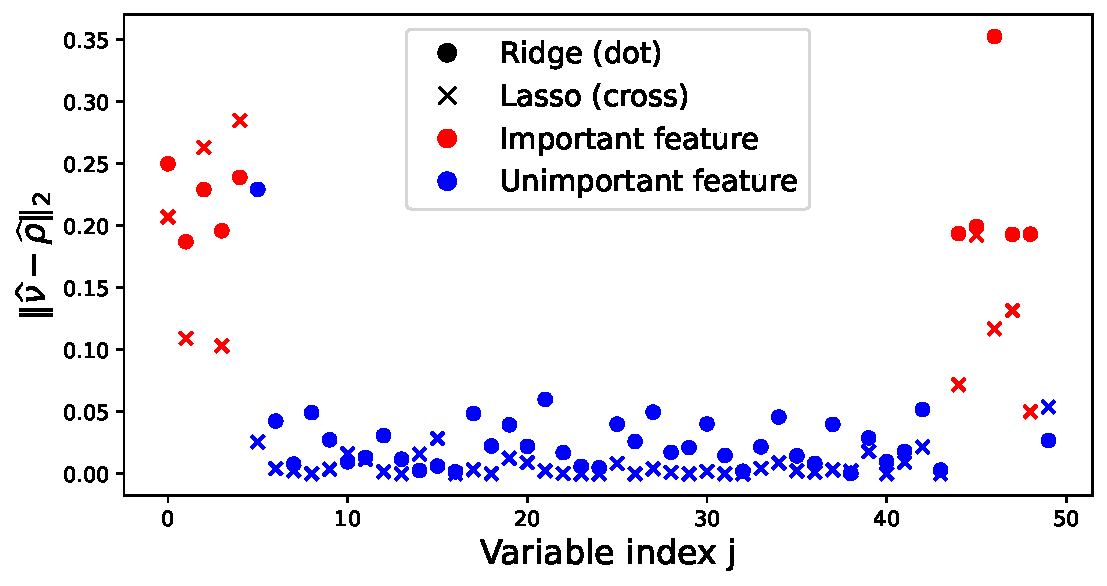
\includegraphics[width=0.45\textwidth]{images/new_exp/stability_ridge_lasso.pdf}
    \caption{\textbf{Optimization stability.} Data are generated from $z = \chi\beta + \epsilon$, where $\beta$ is $0.25$-sparse with important features grouped in blocks of 5 sampled uniformly. We set $n = 300$, $p = 50$, noise level at $\|\chi\beta\|/2$ and $\chi \sim \mathcal{N}(0,\Sigma)$ with $\Sigma_{i,j} = 0.6^{|i-j|}$. The $y$-axis shows the difference between the model coefficients with and without the $x$-axis coordinate.
%. The figure shows the difference between the imputer without coordinate $j$ ($\widehat{\nu}_j$) and with coordinate $j$ ($\widehat{\rho}_j$): red points correspond to important coordinates, blue points to non-important ones. Dots indicate Ridge imputers; crosses indicate Lasso imputers.
 }
    \label{fig:lasso_ridge_stability}
\end{figure}

 
% \ar{Introduce the plot with the coefficients difference and in the appendix the AUC plot}
 
 
 \subsection{Distribution control}\label{sect:Wassers}
 
%The validity of the method relies on the fact that, under the null hypothesis, the two imputers $\widehat{\rho}_j$ and $\widehat{\nu}_j$ are sufficiently close. Indeed, when these estimators are close, both their predictions and the residuals from which we sample will also be similar. Consequently, the two sampling schemes will produce observations that are independent and drawn from the same distribution. Since our statistic is based on their difference, this ensures the required exchangeability. 

The validity of the method relies on the fact that, under the null, the two imputers $\widehat{\rho}_j$ and $\widehat{\nu}_j$ are sufficiently close. Then, both their predictions and the residuals from which we sample are similar, so the two sampling schemes yield observations that are iid. Since our test statistic is based on their difference, this guarantees the required exchangeability.


%In the previous section, we established that the estimators are close through a finite-sample bound on the difference between the coefficients of a regularized ERM when trained with or without an uninformative covariate. In this section, we connect this parameter-level stability to distributional stability by bounding, in Wasserstein distance, the distributions from which we sample. 

%We recover the notation used for the Semi-knockoffs: $\widehat{\nu}_j$ is the regression of $X^j$ on $X^{-j}$, and $\widehat{\rho}_j$ is the regression of $X^j$ on $(X^{-j}, y)$. We denote by $\hat{P}_1^j$ and $\hat{P}_2^j$ the distributions induced by sampling with $\widehat{\nu}_j$ and $\widehat{\rho}_j$, respectively, that is, the laws of $\widetilde{X}'^{(j)}_1$ and $\widetilde{X}'^{(j)}_2$. We work under the assumptions of the previous section and additionally assume that the predictive model is regular enough, satisfying a Lipschitz condition, together with a Lipschitz assumption on the loss with respect to its prediction argument, as in~\cite{opt_error}.
 
We recover the Semi-knockoffs notation: $\widehat{\nu}_j$ is the regressor of $X^j$ on $X^{-j}$, and $\widehat{\rho}_j$ the one of $X^j$ on $(X^{-j}, y)$. We denote by $\hat{P}_1^j$ and $\hat{P}_2^j$ the distributions induced by sampling with $\widehat{\nu}_j$ and $\widehat{\rho}_j$, respectively, that is, the laws of \[
l(\widehat{m}(\widetilde{X}'^{(j)}_1), y)
\quad\text{and}\quad
l(\widehat{m}(\widetilde{X}'^{(j)}_2), y).
\] We work under the assumptions of the previous section and also assume that the model is sufficiently regular, satisfying a Lipschitz condition, together with a Lipschitz loss on its prediction argument, as in~\citet{opt_error}.

 
 
 \begin{theorem}[$\mathcal{W}_1$ control]
 For $j \in \mathcal{H}_0$, under Theorem \ref{thm:opt_stab} assumptions and that model $\widehat{m}$ and loss in the prediction argument are Lipschitz, we have, with probability at least $1-\delta$, that
 \begin{align*}
     \mathcal{W}_1(\hat{P}_1^j, \hat{P}_2^j)\leq O_P\left(\sqrt{\frac{\mathrm{log}(1/\delta)}{n}}\right).
 \end{align*}\label{theo:W_1conv}
 \end{theorem}
%
 This result connects the parameter-level stability from Theorem \ref{thm:opt_stab} to distributional stability by bounding, in Wasserstein distance, the distributions from which we sample.
 
 %In Figure~\ref{fig:fdp_illustration}, we observe that in practice the sampling scheme effectively preserves the required symmetry under the null. This is reflected by the distribution of the null features (left), which is approximately symmetric around 0. As a result, the knockoff threshold successfully controls the FDR across standard ML models. Moreover, the important features exhibit a distribution that is clearly separated from that of the nulls, yielding a powerful testing procedure.

 

 \subsection{Double Robustness}\label{sect:DR}
 %
%\citet{reyerolobo2025conditionalfeatureimportancerevisited} introduced the concept of \emph{double robustness} for the CFI, which similarly is based on an estimated model $\widehat{m}$ and a conditional sampler $\widehat{P}$. They proposed two perspectives for this double robustness. The first one was a general principle: having either a good model $\widehat{m}$ or a good conditional sampler $\widehat{P}$ is sufficient to detect that the coordinate is not important. The second perspective was proposed specifically for a Gaussian linear model, when using the regression conditional sampler based on $\widehat{\nu}$. It was shown that when both $\widehat{m}$ and $\widehat{\nu}$ are well estimated, the convergence to zero is faster — in particular, quadratic rather than linear. Here, we generalize this latter approach and, assuming smoothness of the model $\widehat{m}$, we show that the convergence decay of both models accumulates to achieve this faster rate.
%

\citet{reyerolobo2025conditionalfeatureimportancerevisited} introduced the concept of \emph{double robustness} for the CFI, which is similarly based on an estimated model $\widehat{m}$ and conditional sampler $\widehat{P}$. 
%
%They proposed two different perspectives\bt{Do we need to insist on both. we seem to follow the argument of this paper too closely }. The first was a general principle: having either a good model $\widehat{m}$ or a good conditional sampler $\widehat{P}$ is sufficient to detect whether a coordinate is not important. 
They showed that, for the Gaussian linear model and using the regression-based conditional sampler $\widehat{\nu}$, when both $\widehat{m}$ and $\widehat{\nu}$ are well estimated, the CFI converges to zero at a faster rate (quadratic rather than linear) under the null.
Here, we generalize this perspective and, under smoothness assumptions on $\widehat{m}$, show that the decay rates associated with the two models compound, yielding this faster convergence.
%\cite{reyerolobo2025conditionalfeatureimportancerevisited} introduced the concept of \emph{double robustness} for the general CFI. This CFI is based on an estimated function $\widehat{m}$ and a conditional sampler $\widehat{P}$. They proposed two perspectives for this double robustness. 
%The first one was a general principle: for a coordinate under the null hypothesis, having either a good model $\widehat{m}$ or a good conditional sampler $\widehat{P}$ is sufficient to detect that the coordinate is not important. 
%
%The second perspective was proposed specifically for a linear Gaussian model, using the conditional sampler of the CPI (\cite{chamma2024statistically}) based on $\widehat{\nu}$. It was shown that when both $\widehat{m}$ and $\widehat{\nu}$ are well estimated, the convergence to zero is faster — in particular, quadratic rather than linear. 
%In the next result, we generalize this latter approach and, assuming smoothness of the model $\widehat{m}$, we show that the convergence decay of both models accumulates to achieve this faster rate.
%
 \begin{theorem}[Double Robustness]\label{thm:DR}
 Assume that $j\in \mathcal{H}_0$ and that $t\to l(t, y)$ is $C^2$ with bounded derivatives. Assume also that $\widehat{m}$ is differentiable in the $j$-coordinate and denote by $a_n:=\partial_{x^j}\widehat{m}(X^{-j}, t)$ for a $t$ between $\widetilde{X}'^{j}$ and $\widetilde{X}^j$. Assume that $\widehat{\nu}-\nu=O_P(b_n)$. Then, $$l(\widehat{m}(\widetilde{X}'), y)-l(\widehat{m}(\widetilde{X}), y)=O_P(a_n b_n).$$
 \end{theorem}
%For a faster convergence rate, we require $a_n$ to converge to $0$. This can be interpreted as an \emph{insensitivity} to the unimportant coordinates. Since $j \in \mathcal{H}_0$, the theoretical model does not depend on this feature and $\partial_{x^j} m(X) = 0$. For instance, if $\widehat{m}$ converges to $m$ in $C^1$, this condition is satisfied. 
%
%In practice, this means that the model must smoothly detect that the coordinate is not important. However, as we will see in the next section, this differentiability is not even necessary: we still benefit from the faster convergence rate when using models such as Random Forests, which are not continuous. Indeed, the identifiability of important features in Random Forests has been a key property used to establish their consistency, and in particular, their adaptability to sparse settings (\cite{Scornet_2015ConsistencyRF, pmlr-v130-klusowski21b}). Other methods, such as Neural Networks, can be trained with an explicit penalization on the gradients to improve generalization (\cite{zhao2022penalizing}). However, as we will show below, this penalization is not even necessary to achieve the faster convergence.
%
As we will see in the next section, strict differentiability is not necessary in practice. For instance, with Random Forests, we still observe faster convergence. Indeed, several consistency results have highlighted their adaptability to sparse settings, showing that splits are rarely made on null features \cite{Scornet_2015ConsistencyRF, pmlr-v130-klusowski21b}, leading to the corresponding feature being effectively insignificant in the model.
%We still benefit from the faster convergence rate when using models such as Random Forests, which are not continuous. Their ability to identify important features is a key property that has been used to establish their consistency and adaptability to sparse settings \cite{Scornet_2015ConsistencyRF, pmlr-v130-klusowski21b}. 
Other methods, such as Neural Networks, can be trained with an explicit penalization on the gradients to improve generalization \cite{zhao2022penalizing}. However, as seen below, this is not necessary to achieve the faster rate.
%
\begin{remark}
%this indeed generalizes the faster convergence rates of the Gaussian linear model obtained in \cite{reyerolobo2025conditionalfeatureimportancerevisited}. Specifically, since the Gaussian distribution satisfy their additive innovation assumption, the conditional distribution can be computed as the regression of the coordinate on the others and addition of an independent noise. For $\widehat{m}(X) = \widehat{\beta}^\top X$, we have $\partial_{x^j}\widehat{m}(X) = \widehat{\beta}^j$, which, under the null hypothesis, is centered around $0$ with a variance of order $O(1/n)$. This gives the desired result, since $\widehat{\nu}$ also achieves the same parametric rate. Moreover, the same reasoning extends naturally to any generalized linear model.
This indeed generalizes the faster rates of the Gaussian linear model obtained in \citet{reyerolobo2025conditionalfeatureimportancerevisited}. Specifically, for $\widehat{m}(X) = \widehat{\beta}^\top X$, we have $\partial_{x^j}\widehat{m}(X) = \widehat{\beta}^j$, which, under the null hypothesis, is centered around $0$ with variance of order $O(1/n)$. Moreover, using Gaussianity, $\nu$ is linear. This yields the desired result, since $\widehat{\nu}$ also achieves the same parametric rate. The same reasoning extends naturally to any generalized linear model.
\end{remark}
%
%We note that this indeed generalizes the faster convergence rates of the Gaussian linear model obtained in \cite{reyerolobo2025conditionalfeatureimportancerevisited}. Specifically, they first showed that for a Gaussian distribution, the model can be rewritten in terms of the additive innovation, i.e. the conditional distribution computed as the regression of the coordinate on the others and addition of an independent noise term. For $\widehat{m}(X) = \widehat{\beta}^\top X$, we have $\partial_{x^j}\widehat{m}(X) = \widehat{\beta}^j$, which, under the null hypothesis, is centered around $0$ with a variance of order $O(1/n)$. This gives the desired result, since $\widehat{\nu}$ also achieves the same parametric rate. Moreover, the same reasoning extends naturally to any generalized linear model. 
%Finally, from the proof, we also observe that the assumptions on the loss function could be relaxed to merely require Lipschitz continuity.
%\pn{would be worth formalizing this?}
\subsection{Applications of double robustness to Semi-knockoffs}\label{sect:conject}
 
 
%We observe that the main property required for the validity of Semi-knockoffs is the \emph{exchangeability under the null}, which implies that the sign of the test statistic is uniform. This property arises from having $X_1$ and $X_2$ sampled independently from the same distribution. Thus, if both $\widehat{\rho}$ and $\widehat{\nu}$ are accurate, they both equal $\nu$, since under the null $\rho(X^{-j}, y):=\e{X^j\mid X^{-j}, y}=\e{X^j\mid X^{-j}} =: \nu(X^{-j})$. Consequently, for any $\widehat{m}$, we have
%Note that the validity of Semi-knockoffs mainly relies on the \emph{exchangeability under the null}. This property follows from $X_1$ and $X_2$ being sampled independently from the same distribution and that if both $\widehat{\rho}$ and $\widehat{\nu}$ are accurate, they both equal $\nu$, since under the null $\rho(X^{-j}, y) := \mathbb{E}[X^j \mid X^{-j}, y] = \mathbb{E}[X^j \mid X^{-j}] =: \nu(X^{-j}).$ Consequently, for any $\widehat{m}$, we have
Note that the validity of Semi-knockoffs mainly relies on \emph{exchangeability under the null}. This property follows from $X_1$ and $X_2$ being sampled independently from the same distribution, and from the fact that under the null
$\rho(X^{-j}, y) := \mathbb{E}[X^j \mid X^{-j}, y] = \mathbb{E}[X^j \mid X^{-j}] =: \nu(X^{-j}).$ Consequently, for any model $\widehat{m}$, we have
%
\[
\mathrm{sign}\left(l(\widehat{m}(\widetilde{X}_1), y) - l(\widehat{m}(\widetilde{X}_2), y)\right) \;\overset{d}{=}\; \epsilon^j,
\]
%
where $\epsilon^j \sim \mathcal{U}(\{-1, +1\})$ is a Rademacher r.v.  

We would like the same result to hold with high probability for the empirical counterparts $\widetilde{X}'_1$ and $\widetilde{X}'_2$ based on $\widehat{\nu}$ and $\widehat{\rho}$. We conjecture that this is the case, based on a double robustness argument. Indeed, we expect that the sign of the empirical difference matches the sign of the theoretical one, yielding the desired independent Rademacher variable. Formally, if we arbitrarily assume that the difference is positive, i.e.,
\begin{align}
    l(\widehat{m}(\widetilde{X}_1), y)- l(\widehat{m}(\widetilde{X}_2), y)>0,\label{eq:conj_Semi_KO}
\end{align}
we expect the same sign for the empirical counterparts. This expectation is justified because the difference in \eqref{eq:conj_Semi_KO} is of the order of the insensitivity of the model $\widehat{m}$ with respect to the $j$-th coordinate, while the differences 
%\[
%l(\widehat{m}(\widetilde{X}'_1), y) > l(\widehat{m}(\widetilde{X}'_2), y).
%\]
%is of the order of the insensitivity of the model $\widehat{m}$ with respect to the $j$-th coordinate, while the differences 
\[
l(\widehat{m}(\widetilde{X}_1), y) - l(\widehat{m}(\widetilde{X}'_1), y) \text{ and } l(\widehat{m}(\widetilde{X}_2), y) - l(\widehat{m}(\widetilde{X}'_2), y)
\]
%
decay according to both $\widehat{m}$ and $\widehat{\nu}$ (or $\widehat{\rho}$), then faster, as formalized in Theorem~\ref{thm:DR} and illustrated in Figure~\ref{fig:conjecture}.
%\pn{use blue and orange colors in Figure~\ref{fig:conjecture} ?}
%
\begin{figure}
    \centering
    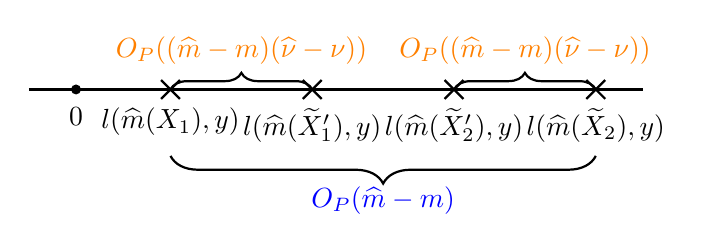
\begin{tikzpicture}[scale=1.2, thick]
    % Points
    \coordinate (O) at (-1,0); % zero
    \coordinate (A) at (0,0);
    \coordinate (B) at (1.5,0);
    \coordinate (C) at (3,0);
    \coordinate (D) at (4.5,0);
    
    % Long horizontal line
    \draw (-1.5,0) -- (5,0);

    % Points
    \fill (O) circle (1.5pt) node[below=3pt] {0};
    \foreach \p/\name in {A/{$l(\widehat{m}(X_1), y)$}, B/{$l(\widehat{m}(\widetilde{X}'_1), y)$}, C/{$l(\widehat{m}(\widetilde{X}'_2), y)$}, D/{$l(\widehat{m}(\widetilde{X}_2), y)$}}
    %\foreach \p/\name in {A/$l(\hat{m}(\widetilde{X}_1), y)$, B/$l(\hat{m}(\widetilde{X}_1), y)$, C/$l(\hat{m}(\widetilde{X}_2), y)$, D/$l(\hat{m}(\widetilde{X}_2), y)$}
        \draw[thick] (\p) node[below=3pt] {\name} 
                      +(-0.1,-0.1) -- +(0.1,0.1) % cross
                      +(-0.1,0.1) -- +(0.1,-0.1);

    % Top braces for a_n
    \draw [decorate, decoration={brace, amplitude=6pt}]
        (A) -- (B) node[midway, yshift=14pt] {\textcolor{orange}{$O_P((\widehat{m}-m)(\widehat{\nu}-\nu))$}};

    \draw [decorate, decoration={brace, amplitude=6pt}]
        (C) -- (D) node[midway, yshift=14pt] {\textcolor{orange}{$O_P((\widehat{m}-m)(\widehat{\nu}-\nu))$}};

    % Bottom brace for b_n (from below A label to below D label)
    \draw [decorate, decoration={brace, amplitude=10pt, mirror}]
        ([yshift=-20pt]A.south west) -- ([yshift=-20pt]D.south east)
        node[midway, yshift=-16pt] {\textcolor{blue}{$O_P(\widehat{m}-m)$}};
\end{tikzpicture}
    \caption{Illustration of the conjecture that $\mathbb{P}\Bigl(l(\widehat{m}(\widetilde{X}'_1), y) > l(\widehat{m}(\widetilde{X}'_2), y) \;\Big|\; l(\widehat{m}(\widetilde{X}_1), y) > l(\widehat{m}(\widetilde{X}_2), y)\Bigr) \;\longrightarrow\; 1,$
thanks to the double robustness property.
}
    \label{fig:conjecture}
\end{figure}
%\bt{For this figure, can you increase the axis label, tiock labels and legend size relative tpo the rest ? This is too small. One easy way to do it is simply to reduce figsize.}
%

Figure~\ref{fig:DR_main} presents the exchangeability idea through double robustness in practice. The same experiment using other learners and studying the effect of independence among training samples is discussed in Appendix~\ref{app:DR_exp}.
%
For a null feature ($X^0$), we plot in blue the distribution capturing only the decay resulting from the sensitivity of $\widehat{m}$ to coordinate $j=0$, obtained by comparing the performance on two independent samples. 
%
We incorporate in orange the decay from both $\widehat{m}$ and the imputers $\widehat{\rho}$ and $\widehat{\nu}$ by comparing the theoretical and empirical residuals from the same sample.
%
Even when employing complex learners for $\widehat{m}$ (Random Forests, Gradient Boosting, and Neural Networks), we observe that the distribution enjoying double robustness (orange) is substantially more concentrated around zero, as established by Theorem~\ref{thm:DR}. 
%
Moreover, in practice, our \emph{knockoff statistic} $W^j_\mathrm{SKO}$ is always based on the distribution  in blue corresponding to the fully estimated models, which remains symmetric and centered at zero across all three complex learners, thereby preserving the desired exchangeability property.
%
%and explains why we expect the exchangeability under the null to be preserved, even when estimating $\widehat{\nu}$ and $\widehat{\rho}$. The experiments are conducted using independent training samples; however, we show in Appendix~\ref{app:DR_exp} that the same property holds when using a single dataset. 
%
%In the figure, we consider a null covariate ($X^0$) and plot the distribution of differences under two scenarios:  
%(i) using only the decay resulting from the sensitivity of $\widehat{m}$ to coordinate $j=0$, obtained by sampling two random residuals (blue distribution), and  
%(ii) incorporating the decay from both $\widehat{m}$, $\widehat{\rho}$, and $\widehat{\nu}$ by comparing the theoretical and empirical residuals from the same sample (orange distribution), and then computing their corresponding predicted losses.  
%
%Moreover, we note that in practice, our \emph{knockoff statistic} is always based on the blue distribution, which corresponds to the fully estimated models. Importantly, this distribution remains symmetric and centered at zero across all three complex learners, thereby preserving the desired exchangeability property in practice.
%
\begin{figure}[t!] 
\hspace*{-5mm}
    \centering
    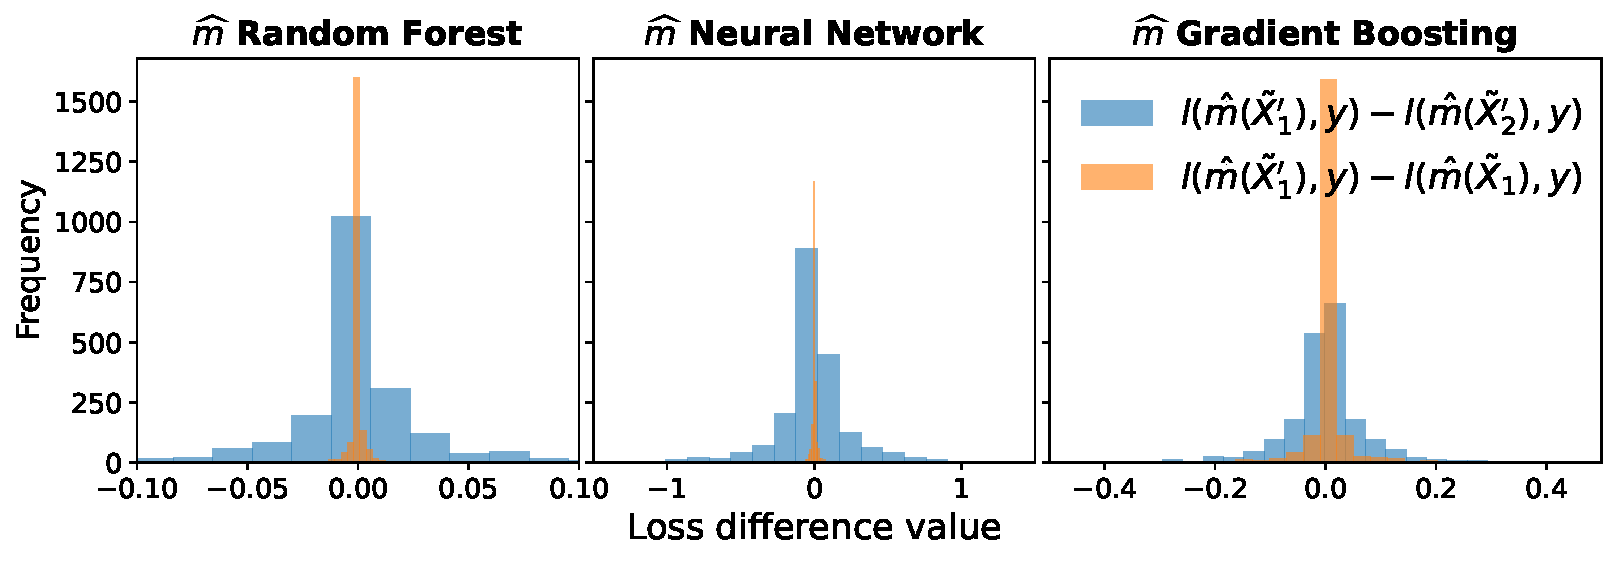
\includegraphics[width=0.52\textwidth]{images/DR/DR_main.pdf}
    \caption{\textbf{Empirical evidence for Double Robustness:} Distribution of the Semi-knockoff statistic, i.e., the difference in loss evaluated at two independently sampled estimated residuals (blue: $l(\widehat{m}(\widetilde{X}_1'), y) - l(\widehat{m}(\widetilde{X}_2'), y)$), and distribution of the difference between the theoretical and estimated imputer (orange: $l(\widehat{m}(\widetilde{X}_1'), y) - l(\widehat{m}(\widetilde{X}_1), y)$) for a null coordinate ($j=0$). The data is sampled from $y = 0.8X^1 + 0.6X^2 + 0.4X^3 + 0.2X^4 + \sin(X^1) + \epsilon$, with $\epsilon \sim \mathcal{N}(0, 0.5)$. We use $n = 2000$ samples with $X \sim \mathcal{N}(0, \Sigma)$, where $\Sigma^{i,j} = 0.5^{|i-j|}$. $\widehat{\nu}$ is a linear model.
 }
    \label{fig:DR_main}
\end{figure}
%\bt{in the caption of the figure, recall what is m, nu and rho}
%
\section{Experiments}

We compare Variable Importance Measures (VIM), such as CFI~\cite{Strobl2008}, with valid tests given by the square-root additive correction \texttt{SCPI(1)\_sqrt} and Wilcoxon test \texttt{SCPI(1)\_Wcx} from~\cite{reyerolobo2025conditionalfeatureimportancerevisited}. We also consider the SAGE value function~\cite{covert2020understanding} with the correction term \texttt{SCPI(100)\_sqrt}, and LOCO~\cite{lei2018} with extra data splitting \texttt{LOCO-W}~\cite{williamson2023general}, the additive correction \texttt{LOCO\_sqrt}~\cite{LocoVSShapley}, or the Wilcoxon test. From Variable Selection, we include dCRT~\cite{liu2022fast} and HRT~\cite{Tansey02012022}. A summary of the methods, references and guarantees in given in Table \ref{tab:summary_CIT} in the Supplementary Materials.

We present only the Semi-knockoffs with the Wilcoxon test \texttt{SKO\_Wcx}, since it is typically more powerful than the sign test. Moreover, it is possible to perform multiple permutations per sample instead of only one; such derandomization strategies have proven beneficial in randomized tests~\cite{shaer23a}. In our experiments, we apply 5 permutations (\texttt{SKO\_Wcx\_p5}). We report power, control, and AUC, and provide time analyses and additional results with other models and settings in Appendix~\ref{app:exps}. FDR control results are given in Appendix \ref{app:fdr_exp}. All experiments are repeated 50 times with $n=300$ and $p=50$. The code is available at %\href{https://anonymous.4open.science/r/Semi_KO-6224}{https://anonymous.4open.science/r/Semi\_KO-6224}.
\href{https://github.com/AngelReyero/loss_based_KO}{https://github.com/AngelReyero/loss\_based\_KO}
\subsection{Simulated data}

In Figure~\ref{fig:main_adj_gb} we study a linear setting with \textit{adjacent support}. 
We first observe that VIMs are too restrictive to make discoveries: they typically rely on asymptotic guarantees, which leads some methods (e.g.\ \texttt{LOCO-W}) to fail to control the type-I error, and their reliance on decay rates results in low power. 
In contrast, variable selection methods enjoy finite-sample control and are substantially more powerful. 
Finally, we note a clear advantage in avoiding sample splitting, as the HRT is noticeably less powerful than methods that do not split the sample.
%
\begin{figure}
    \centering
    %\makebox[\textwidth][l]{%
    \hspace{-1.5em}%
    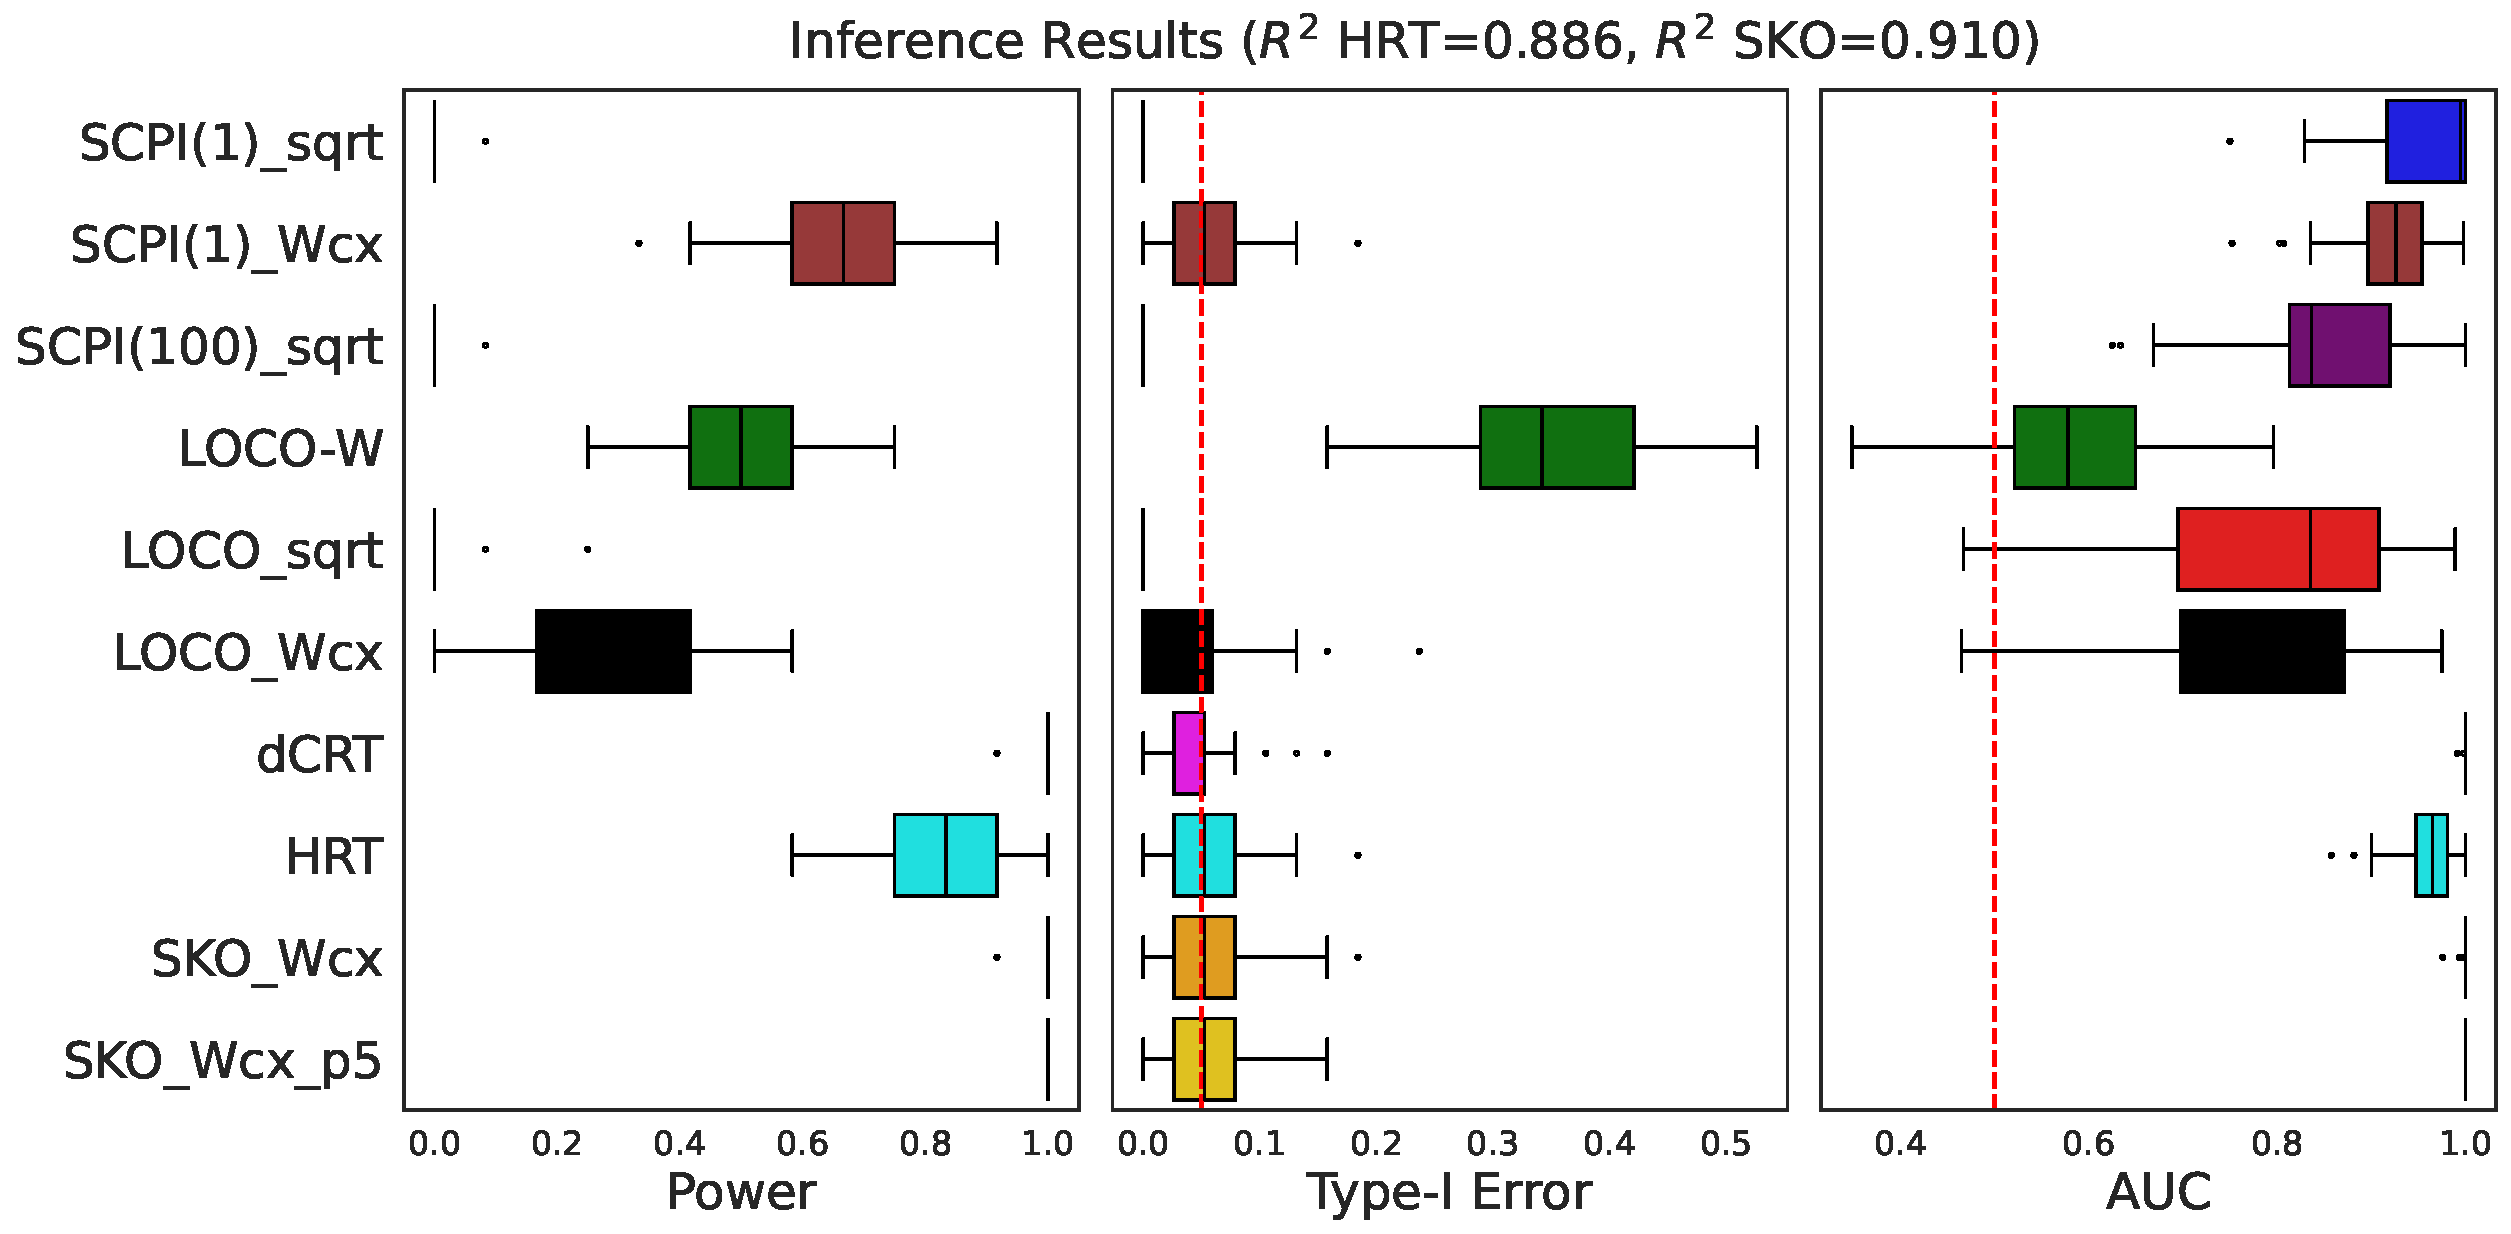
\includegraphics[width=0.5\textwidth]{images/experiments_p_val/main_adjacent_GB.pdf}
    \caption{\textbf{Type-I error with adjacent support.} Let $X \sim \mathcal{N}(0,\Sigma)$ with $\Sigma^{ij} = 0.6^{|i-j|}$, and $y = \beta^\top X + \epsilon$, where the first $0.25p$ coordinates of $\beta$ lie in $[1,2]$ and the remaining are zero, with $\epsilon \sim \mathcal{N}(0,1)$. The black-box pretrained model $\widehat{m}$ is a gradient boosting, achieving $R^2 = 0.886$ with a train-test split and $R^2 = 0.91$ without split.
    }
    \label{fig:main_adj_gb}
\end{figure}
%
In Figure~\ref{fig:main_masked_nn} we study a \textit{masked correlation} setting in which an important feature is strongly correlated with a null feature. 
As before, we observe that the corrections used in VIMs are too restrictive, highlighting the need for valid testing procedures that can still accommodate arbitrary models. 
In contrast, the dCRT exhibits low power: its two-step feature-splitting strategy, used to speed up computation, prevents it from capturing all relevant interactions, and thus the first distillation generally remove most of the signal from the important feature. 
Finally, we observe a substantial gain from derandomization of the Semi-knockoffs: using only five permutations already yields the most powerful procedure.
%
\begin{figure}
    \centering
    \hspace{-1.5em}
    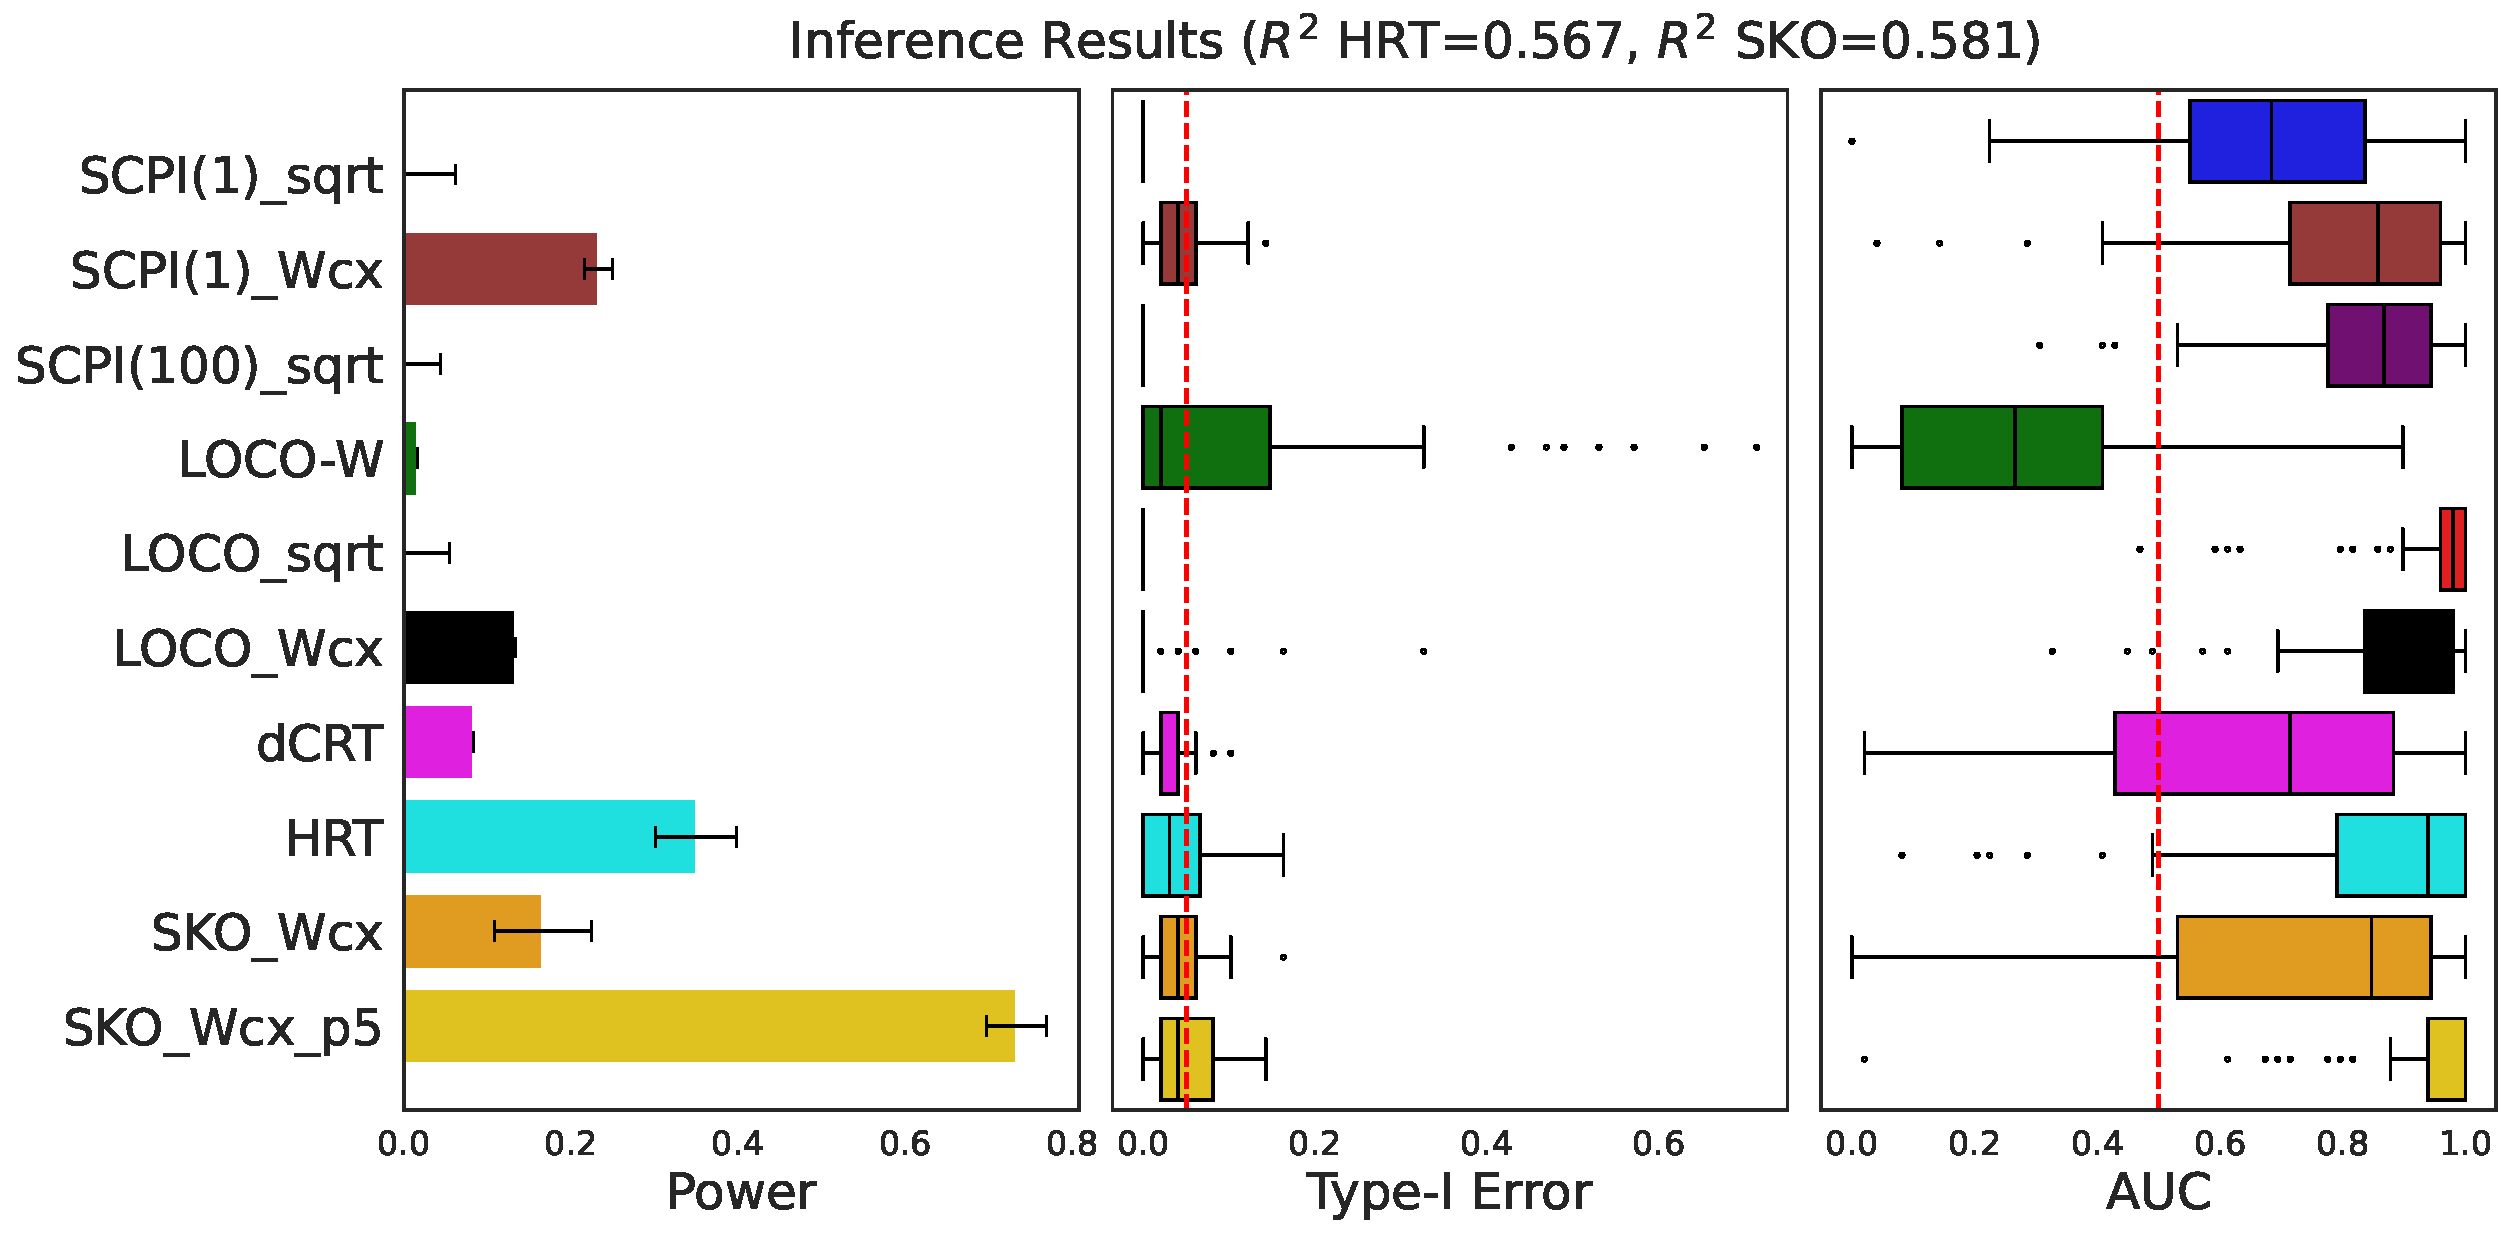
\includegraphics[width=0.5\textwidth]{images/experiments_p_val/main_masked_corr_NN.pdf}
    \caption{\textbf{Type-I error with masked correlation.} Let $X \sim \mathcal{N}(0,\Sigma)$ with $\Sigma_{ij} = 0.6^{|i-j|}$. A unique relevant coordinate $l$ is sampled and $y = X_l + 0.5\,\epsilon_1$, where $\epsilon_1 \sim \mathcal{N}(0,1)$. A correlated null variable is created as $X_{l-1} = X_l + 0.5\,\epsilon_2$, with $\epsilon_2 \sim \mathcal{N}(0,1)$. The black-box pretrained model $\widehat{m}$ is a neural network, achieving $R^2 = 0.567$ with a train-test split and $R^2 = 0.581$ without split.
 }
    \label{fig:main_masked_nn}
\end{figure}

\subsection{Real data}
We also compare the methods on real data to evaluate their discovery capability. For this, we use the Wisconsin Breast Cancer dataset \cite{wdbc1995}; see Appendix~\ref{app:wdbc} for more details on the data and experiments. Since the true set of important features is unknown, we add an extra null feature correlated at $0.6$ with the original features. This allows us to estimate the type-I error in Figure~\ref{fig:main_real} using this artificial feature, indicated on the right of each plot. We present results using Random Forests, Neural Networks, and Gradient Boosting. Similar to the simulated data, the proposed method can make discoveries while controlling the error; derandomization slightly increases power. Importantly, it exhibits stable power across models and consistent numbers of discoveries, unlike other methods whose results vary significantly with the random seed.


\begin{figure}
    \centering
    \hspace{-1.5em}
    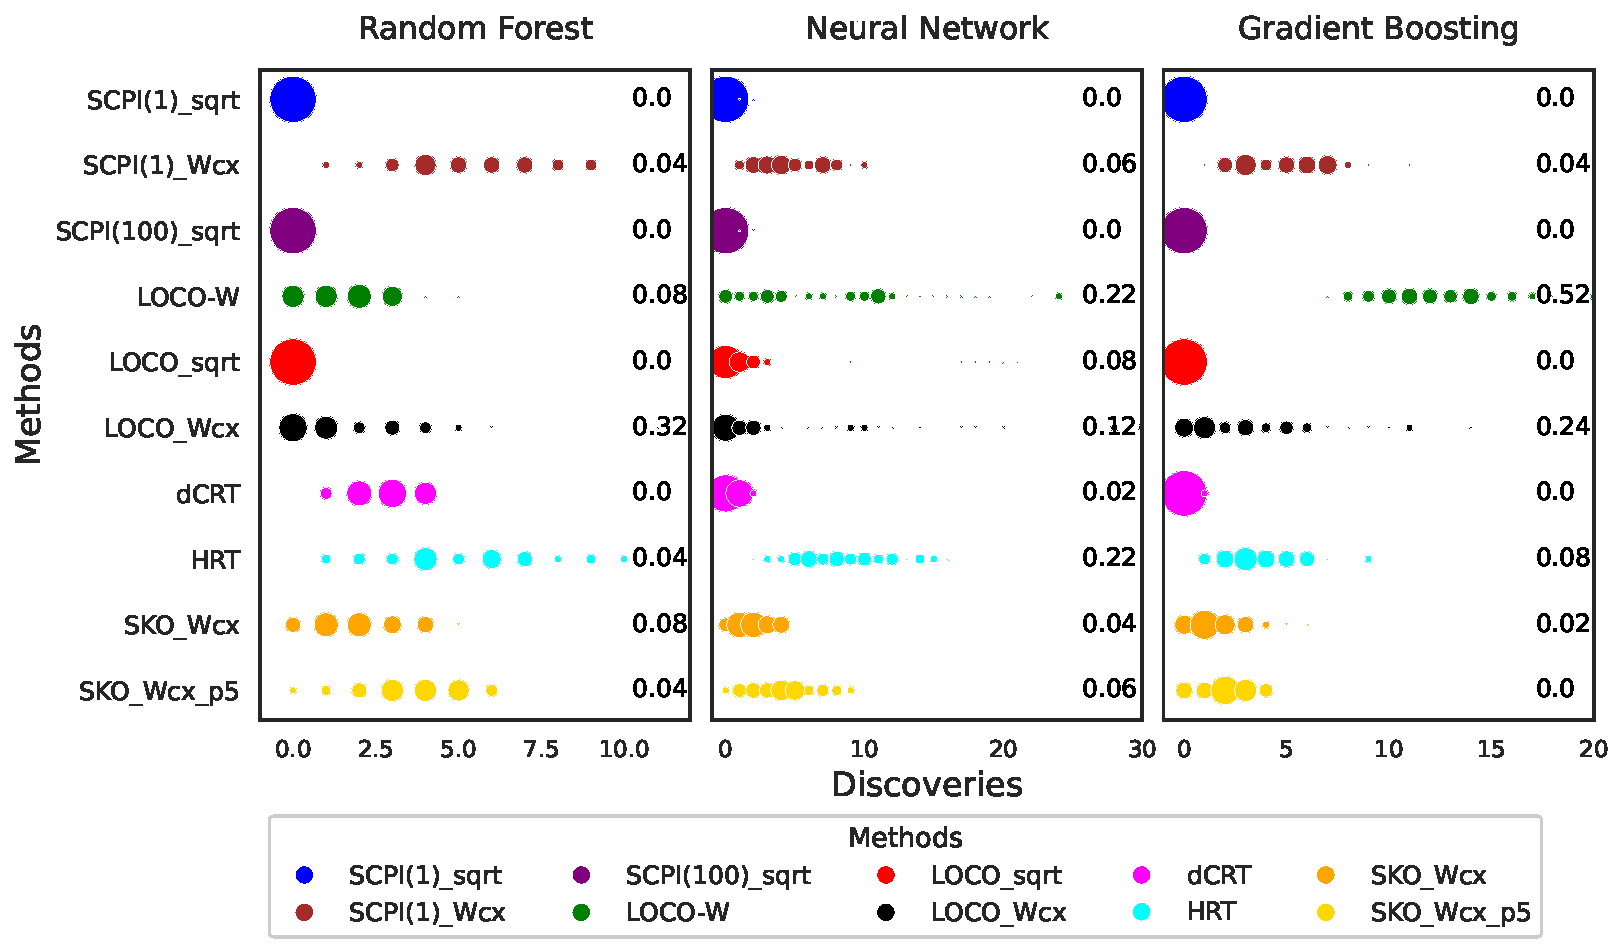
\includegraphics[width=0.5\textwidth]{images/real_data/power_wdbc_GB.pdf}
    \caption{\textbf{Discoveries on real data across ML models.} The type-I error (shown to the right of each plot) is estimated using an artificial null feature correlated at $0.6$ with the original features. Semi-knockoffs make discoveries while controlling the error.
}
    \label{fig:main_real}
\end{figure}

%\subsection{FDR control}

%To study FDR control, we also include standard \texttt{Knockoffs}~\cite{candes2018panning}. For the procedures that output $p$-values (\texttt{HRT}, \texttt{dCRT}, and \texttt{SKO-Wcx}), we apply a standard Benjamini-Hochberg correction~\cite{BH}. In Figure~\ref{fig:main_KO_nongaus} we present the adjacent linear setting where the covariates are \textit{heavy-tailed} rather than Gaussian. We observe that \texttt{Knockoffs} fail to control FDR under this non-Gaussian design,\pn{je ne vois quasiment pas la barre noire dans le boxplot bleu des Knockoffs} highlighting the need for procedures that avoid generating knockoff variables directly. For Semi-knockoffs, we further observe a slight improvement due to derandomization, and that using the knockoff threshold yields greater power while controlling the FDR.


%\begin{figure}
%    \centering
 %   \includegraphics[width=0.5\textwidth]{images/exp_KO/main_nongauss_NN.pdf}
  %  \caption{\textbf{FDR with heavy-tailed $X$.} Let $X = \Sigma^{1/2} Z$, where $Z$ has i.i.d.\ t-Student entries $Z_{ij} \sim t_3$ and $\Sigma_{ij} = 0.6^{|i-j|}$.  We generate $y = \beta^\top X + \epsilon$, where the first $0.25p$ coordinates of $\beta$ lie in $[1,2]$ and the remaining entries are zero, with $\epsilon \sim \mathcal{N}(0,1)$. The black-box pretrained model $\widehat{m}$ is a neural network, achieving $R^2 = 0.832$ with a train-test split and $R^2 = 0.854$ without split.
%}
%    \label{fig:main_KO_nongaus}
%\end{figure}


\section{Discussion}

We have presented \textit{Semi-knockoffs}, a framework for CIT that accommodates any pretrained model and avoids train-test splitting. This is achieved by constructing a test statistic that is symmetric under the null through the creation of two populations: one that incorporates information from the response and one that does not. As a result, the dependence between the model and the distribution under test does not need to be broken; the model is used only as an importance score, similarly to how lasso coefficients are used. This allows us to leverage the  powerful knockoff thresholding procedure without requiring the stringent structural constraints needed to construct knockoff variables and statistics. Moreover, it provides both type-I error and FDR control.

One limitation may come from using a simple model for the imputer incorporating the response. While this remains valid, it may fail to capture richer relationships and break the symmetry with the other imputer under the alternative. Future work will investigate how such imputations and other ways of exploiting information in the response can be combined to further increase statistical power, and whether more complex imputation models can still control the error in practice via double-robustness guarantees similar to those established in this paper. Importantly, note that in the context of missing-data imputation, sampling strategies that condition on both covariates and the response have recently been explored and they have shown substantial improvements~\cite{DAgostinoMcGowan2024}. 
%\bt{Putting this argument as the very end is a bit surprising and the consequence of this observation remains somewhat unclear}.





\section*{Impact Statement}

This paper presents work whose goal is to advance the field of Machine
Learning. There are many potential societal consequences of our work, none
which we feel must be specifically highlighted here.




\bibliography{biblio}
\bibliographystyle{icml2026}

%%%%%%%%%%%%%%%%%%%%%%%%%%%%%%%%%%%%%%%%%%%%%%%%%%%%%%%%%%%%%%%%%%%%%%%%%%%%%%%
%%%%%%%%%%%%%%%%%%%%%%%%%%%%%%%%%%%%%%%%%%%%%%%%%%%%%%%%%%%%%%%%%%%%%%%%%%%%%%%
% APPENDIX
%%%%%%%%%%%%%%%%%%%%%%%%%%%%%%%%%%%%%%%%%%%%%%%%%%%%%%%%%%%%%%%%%%%%%%%%%%%%%%%
%%%%%%%%%%%%%%%%%%%%%%%%%%%%%%%%%%%%%%%%%%%%%%%%%%%%%%%%%%%%%%%%%%%%%%%%%%%%%%%
\newpage
\appendix
\onecolumn


\section{Notation Glossary}\label{sect:glossary}
%\addcontentsline{toc}{section}{Appendix A: Notation Glossary}

\begin{longtable}{p{4cm} p{12cm}}
\textbf{Symbol} & \textbf{Description} \\
\hline
$X\in \mathbb{R}^p$ & Input\\
$X^j\in \mathbb{R}$ & $j$-th input covariate\\
$X^{-j}\in \mathbb{R}^{p-1}$ & Input with the $j$-th covariate excluded\\
$y\in \mathbb{R}$ & Output\\
$x_i$ & $i$-th individual\\
$x_i^{(j)}$ & $i$-th individual with permuted $j$-th covariate\\
$m(X)$ (resp. $m_{-j}(X^{-j})$) & $\e{y\mid X}$ (resp. $\e{y\mid X^{-j}}$)\\
$\widehat{m}$ (resp. $\widehat{m}_{-j}$) & Estimation of $m$ (resp. of $m_{-j}$) \\
$\nu_{j}(X^{-j})$ & $\e{X^j\mid X^{-j}}$\\
$\widehat{\nu}_{j}$ & Estimation of $\nu_{j}$\\
$\rho_{j}(X^{-j}, y)$ & $\e{X^j\mid X^{-j}, y}$\\
$\widehat{\rho}_{j}$ & Estimation of $\rho_{j}$\\
$\widetilde{X}^{(j)}_1$ & Semi-knockoff variable drawn using $\nu_j$\\
$\widetilde{X}^{(j)}_2$ & Semi-knockoff variable drawn using $\rho_j$\\
$\widetilde{X}^{'(j)}_1$ & Semi-knockoff variable drawn using $\widehat{\nu}_j$\\
$\widetilde{X}^{'(j)}_2$ & Semi-knockoff variable drawn using $\widehat{\rho}_j$\\
$\hat{P}_1^j$ & Distribution of $\widetilde{X}^{'(j)}_1$\\
$\hat{P}_2^j$ & Distribution of $\widetilde{X}^{'(j)}_2$\\
$\ell$ & Loss function\\
$\mathcal{W}_1$ & 1-Wasserstein distance\\
$\mathcal{L}$ & Likelihood\\
$T_q$ & Knockoff threshold\\
$W^j_\mathrm{SKO}$ (resp. $\hat{W}^j_\mathrm{SKO}$) & Oracle (resp. Practical) Semi-knockoff statistic\\
$S_\mathrm{SKO}$ (resp. $\hat{S}_\mathrm{SKO}$) & Oracle (resp. Practical) Semi-knockoff selected features\\
$R_n$ & Regularised empirical risk\\
$O_P(a_n)$ & Bounded in probability at a rate of $a_n$. 
\end{longtable}

The superscript $(j)$ is omitted to avoid index overload when $j$ can be inferred from the context. %Also, some notation can be combined; for instance, $\widetilde{x}^{'(j),l}_{i,k}$ denotes the $l$-th coordinate of $\widetilde{x}^{'(j)}_{i,k}$.


\section{Explicit definitions}\label{sect:LOCO_CFI_MX}

For the sake of space, in this section we provide explicit definitions of the procedures that were introduced in Section~\ref{sect:related_work}.



\subsection{Leave One Covariate Out (LOCO)}

LOCO consists of assessing the importance of a feature by studying the performance drop when the model is trained without it ($\widehat{m}_{-j}$).


\begin{definition}[LOCO] Given $j$, a loss $\ell$, a regressor $\widehat{m}$ of $y$ given $X$, a regressor $\widehat{m}_{-j}$ of $y$ given $X^{-j}$ and a test set $(X_i, y_i)_{i=1,\ldots n_\mathrm{test}}$, LOCO is defined as
\begin{align*}
    \widehat{\psi}_\mathrm{LOCO}^j=\frac{1}{n_{\mathrm{test}}}\sum_{i=1}^{n_{\mathrm{test}}}\ell\left(\widehat{m}_{-j}(x_{i}^{-j}), y_i\right)-\ell\left(\widehat{m}(x_{i}),y_i)\right).
\end{align*}
\end{definition}

\subsection{Conditional Feature Importance (CFI)}\label{app:CFI}

CFI consists of reusing the same model while restricting the information from the feature by breaking its link with the output, while preserving its dependence with the rest of the input to avoid extrapolation.

\begin{definition}[CFI] Given $j$, a loss $\ell$, a regressor $\widehat{m}$ of $y$ given $X$ and a test set $(X_i, y_i)_{i=1,\ldots n_\mathrm{test}}$, CPI is defined as
\begin{align*}
    \widehat{\psi}_{\mathrm{CPI}}^j=\frac{1}{n_{\mathrm{test}}}\sum_{i=1}^{n_{\mathrm{test}}}\ell\left(\widehat{m}(\widetilde{x}_{i}'^{(j)}),y_i\right)-\ell\left(\widehat{m}(x_{i}), y_i\right),
\end{align*}
where the $j$-th coordinate is \textit{conditionally} permuted.
\end{definition}


\subsection{Knockoff definition}\label{append:Knockoff_def}

Knockoffs~\cite{candes2018panning} provides a framework for studying conditional independence testing with FDR control by creating synthetic features that appear feasible but break the link with the output, and then comparing the performance between the knockoff features and the original ones. More formally, it relies on \textit{knockoff variables} $\widetilde{X}$ (Appendix~\ref{app:ko_variables}), which do not preserve the relationship with $y$ but follow the distribution of $X$, a \textit{knockoff statistic} $W$ (Appendix~\ref{app:ko_stat}) that assigns an importance to the feature, and the \textit{knockoff threshold} $T_q$~\eqref{eq:knockoff-threshold}.


\subsubsection{Knockoff variables}\label{app:ko_variables}



\begin{definition}[Model-X knockoffs] For a random variable $X$, it is a new random variable $\widetilde{X}$ constructed satisfying the following two properties:
\begin{enumerate}
    \item For any subset $s\subset \{1,\ldots,p\}$, the original and the knockoff variables are exchangeable, i.e. $(X, \widetilde{X})_{\mathrm{swap}(s)}\overset{d}{=}(X, \widetilde{X})$.
    \item $\widetilde{X}\indep y|X$.
\end{enumerate}\label{def:Model-X_knockoffs}
\end{definition}

We observe that the second property can be obtained by constructing the knockoffs without using the output. Moreover, these imitation variables must satisfy the exchangeability condition that is stronger than merely sampling from the conditional distribution, as it must hold over the joint distribution rather than feature-wise. Consequently, computing knockoffs in practice requires a sequential procedure and cannot be parallelized, in contrast to the CRT. While many methods have been proposed for generating knockoff variables in practice~\cite{sesia2019gene, romano2020deep, bates2021metropolized}, and recent work has established asymptotic FDR control~\cite{fan2025asymptoticfdrcontrolmodelx}, concerns have been raised regarding their finite-sample validity~\cite{blain2025knockoffsfaildiagnosingfixing}.




\subsubsection{Knockoff statistics}\label{app:ko_stat}


\begin{definition}[Feature statistics from \cite{candes2018panning}] It is a vector $\mathbf{W}=(W_1, \ldots, W_p)\in \mathbb{R}^p$ where each coordinate $W_j$ satisfies
\begin{enumerate}
    \item It is a function of the input $X$, the knockoff $\widetilde{X}$ and the output $y$: $W_j=w_j\left(\left[X, \widetilde{X}\right], y\right)$.
    \item It satisfies the flip-sign property: for $s\subset[p]$,
    
    
\[
w_j\left(\left[X, \widetilde{X}\right]_{\mathrm{swap}(s)}, y\right) = 
\begin{cases} 
    w_j\left(\left[X, \widetilde{X}\right], y\right) & \text{if } j\cancel{\in} s,  \\
   -w_j\left(\left[X, \widetilde{X}\right], y\right) & \text{if } j\in s.
\end{cases}
\]
\end{enumerate}
\label{def:knock-statistic}
\end{definition}

This statistic provides a hint of how important the feature is. The most intuitive example is given by the Lasso Coefficient Difference (LCD), which, to assign importance, compares the coefficients of a Lasso regression of $y$ on both $(X, \widetilde{X})$, so that $W^j_{\mathrm{LCD}} := |\hat{\beta}^j| - |\hat{\beta}^{j+p}|$. Then, if the coordinate is important, there is more information in the coefficient for the original feature than for its knockoff counterpart.


%\subsubsection{Shapley Knockoffs: model-agnostic knockoff statistics}\label{sect:ShapKO}
 %\bt{Unclear to me why we introduce it ?}
 
%Building statistics with a model-agnostic procedure that satisfies the antisymmetric condition is not evident. Indeed, one naive approach would be to directly swap the important coordinate with its knockoff counterpart and compute the resulting performance drop~\cite{Watson2021}:

 
% \begin{align}\label{eq:loss_CPI}
%     l\left(\widehat{m}(\widetilde{X}^{(j)}), y\right)-l\left(\widehat{m}(X), y\right).
% \end{align}

%We observe that this is, in particular, a CFI (Appendix~\ref{app:CFI}), since the knockoff variables are conditional samples. However, this only satisfies the antisymmetry property for $s=\{j\}$, whereas antisymmetry must hold for every $s \subset [p]$. Therefore, exchangeability between the statistics is not guaranteed, and neither is FDR control, since there is dependency between the signs across features. One way to overcome this and obtain antisymmetry across all subsets is to construct a statistic inspired by the Shapley values~\cite{Shapley1953}, by computing the contribution of a feature across all subsets:



%\begin{definition}[Shapley-statistic] \label{def:shap-stat}
%    It is the vector $W_\mathrm{Shap}$, where each coordinate $W^j_\mathrm{Shap}$ is given by 
%    \begin{align*}
%        W^j_\mathrm{Shap}:=\sum_{x^1\in\{X^1, \widetilde{X}^1\}\times \ldots\times x^p\in \{X^p, \widetilde{X}^p\}} (y-\widehat{m}(x^1, \ldots, \widetilde{X}^j, \ldots, x^p))^2-(y-\widehat{m}(x^1,\ldots, X^j, \ldots, x^p))^2.
%    \end{align*}
%\end{definition}

%In particular, we do have the antisymmetry and in consequence the FDR control: 

%\begin{theorem}[Shapley-KO FDR control] Given $(X, \widetilde{X})$ as in Definition~\ref{def:Model-X_knockoffs}, with Shapley statistics $W_{\mathrm{Shap}}$ for any model $\widehat{m}$, then for $S_{\mathrm{Shap}} := \{\,j : W^j_{\mathrm{Shap}} \geq T_q \,\}$ we have $\mathrm{FDR}(S_{\mathrm{Shap}}) < q$.
%\end{theorem}

%\begin{proof}

%To prove the validity of the Shapley knockoffs we only need to proove that the Shapley statistic is valid, i.e. it does only depend on $[X, \widetilde{X}], y$ and it needs to be antisymmetric. To see this, we first observe that
%    \begin{align*}
%        W^j_\mathrm{Shap}&=w_j([X, \widetilde{X}], y)\\&:=\sum_{x^1\in\{X^1, \widetilde{X}^1\}\times \ldots\times x^p\in \{X^p, \widetilde{X}^p\}} (y-\widehat{m}(x^1, \ldots, \widetilde{X}^j, \ldots, x^p))^2-(y-\widehat{m}(x^1,\ldots, X^j, \ldots, x^p))^2,
%    \end{align*}
%    therefore, it is obviously a function of the input $X$, the knockoff $\widetilde{X}$ and the output $y$. Then, to prove the flip-sign property,
%    we first observe that for any subset $s\subset\{1, \ldots, p\}$, and for any $l\in s, l\neq j$ we have that $$w_j([X, \widetilde{X}]_{\mathrm{swap}(s)}, y)=w_j([X, \widetilde{X}]_{\mathrm{swap}(s\backslash l)}, y)$$ because of the commutativity of the sum and because $x^l\in\{X^l,\widetilde{X}^l\}$ is equivalent to $x^l\in \{\widetilde{X}^l, X^l\}$. Therefore, we could proceed in this way to discard all the covariates from $s$ but the $j$-th covariate. It the $j$-th covariate is $s$, then we can easily observe the antisymmetry property because of the antisymmetry of the subtraction. Therefore, we have that 
    
%    \[
%w_j\left(\left[X, \widetilde{X}\right]_{\mathrm{swap}(s)}, y\right) = 
%\begin{cases} 
%    w_j\left(\left[X, \widetilde{X}\right], y\right) & \text{if } j\cancel{\in} s,  \\
%   -w_j\left(\left[X, \widetilde{X}\right], y\right) & \text{if } j\in s.
%\end{cases}
%\]

   % Finally, combining all the previous results and using the framework from \cite{candes2018panning}, FDR control is guaranteed.
%\end{proof}


%Nevertheless, similarly to Shapley values for feature importance~\cite{covert2020understanding}, computing all combinations can be computationally infeasible, especially since knockoffs were designed for high-dimensional settings. Moreover, this approach, while accommodating any ML model, still relies on knockoff variables. For these reasons, we have set this approach aside and instead propose the Semi-knockoffs.


\section{Algorithms}\label{sect:pseudocode}

We first present the theoretical Semi-knockoffs, which provide valid type-I error control through nonparametric paired tests (Wilcoxon or Sign test), and then describe the procedure for controlling FDR using the knockoff threshold. We note that, in practice, the procedure is identical, relying on the computation of the regressors $\widehat{\nu}$ and $\widehat{\rho}$ (Algorithm~\ref{alg:semi_knockoffs}).


\subsection{Type-I error algorithm (Semi-KO Sign test/Wilcoxon)}



\begin{algorithm}[H]
\caption{Oracle Semi-knockoffs Sign-Test/Wilcoxon (Semi-KO ST/Wilcox)}
\label{alg:semi_knockoffs_oracle_wcx}
\begin{algorithmic}[1]
%\Require
\item[] \textbf{Input:} Model $\widehat{m}$, data $\{(X_i,y_i)\}_i^n$, significance level $\alpha$, a feature $j$, conditional expectations $\nu_j$ and $\rho_j $
    \item[] Compute theoretical residuals $\epsilon_{j,1} = X^j -\nu_j(X^{-j})$
    \item[] Compute theoretical residuals $\epsilon_{j,2} = X^j - \rho_j(X^{-j}, y)$
    \item[] Sample $\pi_{j,1}$ and $\pi_{j,2}$ permutations of $\{1,\dots,n\}$
    \item[] Construct 
    \begin{align*}
        \widetilde{X}^{(j)}_{1,i}
        &= \nu_j(X^{-j}_i)
        + \epsilon_{j,1,\pi_{j,1}(i)}\\
        \widetilde{X}^{(j)}_{2,i}
        &= \rho_j(X^{-j}_i, y_i)
        + \epsilon_{j,2,\pi_{j,2}(i)}
    \end{align*}
    \item[] Compute nonparametric paired test (Sign-test/Wilcoxon) between %$\hat{W}^j_\mathrm{SKO}$
    \[
        \left\{l\bigl(\widehat{m}(\widetilde{X}^{(j)}_{1,i}), y_i\bigr)\right\}
        \text{ and }
        \left\{l\bigl(\widehat{m}(\widetilde{X}^{(j)}_{2,i}), y_i\bigr)\right\}
    \]
\item[] \textbf{Return} the computed p-value
\end{algorithmic}
\label{alg:theo-semi-KO-wilcox}
\end{algorithm}



\subsection{Oracle Semi-knockoffs}


\begin{algorithm}[H]
\caption{Oracle Semi-knockoffs (Semi-KO)}
\label{alg:semi_knockoffs_oracle}
\begin{algorithmic}[1]
%\Require
\item[] \textbf{Input:} Model $\widehat{m}$, data $\{(X_i,y_i)\}_i^n$, significance level $q$, conditional expectations $\nu_j$ and $\rho_j $ for every feature $j$
\item[] \textbf{For} $j = 1,\dots,p$
    \item[] \quad Compute theoretical residuals $\epsilon_{j,1} = X^j -\nu_j(X^{-j})$
    \item[] \quad Compute theoretical residuals $\epsilon_{j,2} = X^j - \rho_j(X^{-j}, y)$
    \item[] \quad Sample $\pi_{j,1}$ and $\pi_{j,2}$ permutations of $\{1,\dots,n\}$
    \item[] \quad Construct 
    \begin{align*}
        \widetilde{X}^{(j)}_{1,i}
        &= \nu_j(X^{-j}_i)
        + \epsilon_{j,1,\pi_{j,1}(i)}\\
        \widetilde{X}^{(j)}_{2,i}
        &= \rho_j(X^{-j}_i, y_i)
        + \epsilon_{j,2,\pi_{j,2}(i)}
    \end{align*}
    \item[] \quad Compute the statistic %$\hat{W}^j_\mathrm{SKO}$
    \[
    \quad W^j_\mathrm{SKO} = \frac{1}{n} \sum_{i=1}^{n}
    \Bigl( 
        l\bigl(\widehat{m}(\widetilde{X}^{(j)}_{1,i}), y_i\bigr)
        - 
        l\bigl(\widehat{m}(\widetilde{X}^{(j)}_{2,i}), y_i\bigr)
    \Bigr)
    \]
\item[] Compute knockoff threshold $T_q$ as in \eqref{eq:knockoff-threshold}
\item[] \textbf{Return} 
\[
S_{\mathrm{SKO}}
=
\bigl\{
j : W^j_\mathrm{SKO} \ge T_q
\bigr\}.
\]
\end{algorithmic}
\label{alg:theo-semi-KO}
\end{algorithm}

\subsection{Semi-knockoffs}

\begin{algorithm}[H]
\caption{Semi-knockoffs (SKO)}
\label{alg:semi_knockoffs}
\begin{algorithmic}[1]
%\Require
\item[] \textbf{Input:} Model $\widehat{m}$, data $\{(X_i,y_i)\}_i^n$, significance level $q$
\item[] \textbf{For} $j = 1,\dots,p$
    \item[] \quad \textbf{(Regression 1)} Fit $\widehat{\nu}_j \approx \mathbb{E}[X^j \mid X^{-j}]$
    \item[] \quad \textbf{(Regression 2)} Fit $\widehat{\rho}_j \approx \mathbb{E}[X^j \mid X^{-j}, y]$
    \item[] \quad Compute residuals $\widehat{\epsilon}_{j,1} = X^j - \widehat{\nu}_j(X^{-j})$
    \item[] \quad Compute residuals $\widehat{\epsilon}_{j,2} = X^j - \widehat{\rho}_j(X^{-j}, y)$
    \item[] \quad Sample $\pi_{j,1}$ and $\pi_{j,2}$ permutations of $\{1,\dots,n\}$
    \item[] \quad Construct 
    \begin{align*}
        \widetilde{X}'^{(j)}_{1,i}
        &= \widehat{\nu}_j(X^{-j}_i)
        + \widehat{\epsilon}_{j,1,\pi_{j,1}(i)}\\
        \widetilde{X}'^{(j)}_{2,i}
        &= \widehat{\rho}_j(X^{-j}_i, y_i)
        + \widehat{\epsilon}_{j,2,\pi_{j,2}(i)}
    \end{align*}
    \item[] \quad Compute the statistic %$\hat{W}^j_\mathrm{SKO}$
    \[
    \quad\hat{W}^j_\mathrm{SKO} = \frac{1}{n} \sum_{i=1}^{n}
    \Bigl( 
        l\bigl(\widehat{m}(\widetilde{X}'^{(j)}_{1,i}), y_i\bigr)
        - 
        l\bigl(\widehat{m}(\widetilde{X}'^{(j)}_{2,i}), y_i\bigr)
    \Bigr)
    \]
\item[] Compute knockoff threshold $T_q$ as in \eqref{eq:knockoff-threshold}
\item[] \textbf{Return} 
\[
\widehat{S}_{\mathrm{SKO}}
=
\bigl\{
j : \hat{W}^j_\mathrm{SKO} \ge T_q
\bigr\}.
\]
\end{algorithmic}
\label{alg:semi-KO}
\end{algorithm}
\section{Mathematical tools}
 
 
In this section, we present some mathematical tools and results from high-dimensional probability that were used in our analysis. They are mainly obtained from \citet{Vershynin_2018}. The first definitions concern the sub-Gaussian and sub-exponential norms:


\begin{definition}[Subgaussian norm]\label{def:subgaussian_norm}
$\|X\|_{\psi_2}=\mathrm{inf}\{K>0, \e{\mathrm{exp}X^2/K^2}\leq 2\}$.
\end{definition}
%\bt{IIRC the Subgaussian hypothesis was not mentioned in the main text ?}

\begin{definition}[Subexponential norm]
$\|X\|_{\psi_1}=\mathrm{inf}\{K>0, \e{\mathrm{exp}|X|/K}\leq 2\}$.
\end{definition}

Also, Lemma 2.8.6 from \citet{Vershynin_2018} gives that the product of subgaussians is subexponential.
\begin{lemma}[Subgaussian $\times$ subgaussian = subexponential]\label{lemm:subG_x_subG} If $X$ and $Y$ are subgaussian, then $XY$ is subexponential, and 
$\|XY\|_{\psi_1}\leq \|X\|_{\psi_2}\|Y\|_{\psi_2}$.

\end{lemma}

Similarly to sub-Gaussian random variables, there is an analogous Bernstein-type result for sub-exponential variables (Theorem 2.9.1 in \citet{Vershynin_2018}):
\begin{theorem}[Subexponential Bernstein]\label{th:bernstein} Let $X_1, \ldots, X_n$ independent, mean zero subexponential random variables. Then, for every $t\geq 0$, 
$$\mathbb{P}\left(\left|\sum_{i=1}^n X_i\right|\geq t\right)\leq 2\mathrm{exp}\left(-c\mathrm{min}\left(\frac{t^2}{\sum_{i=1}^n\|X_i\|^2_{\psi_1}}, \frac{t}{\mathrm{max}_i\|X_i\|_{\psi_1}}\right)\right)$$
where $c>0$ is an absolute constant.
\end{theorem}






\section{Proofs}
\subsection{Semi-knockoffs type-I error control: Theorem \ref{thm:type-I-control}}


\begin{proof}
Since the algorithm relies on a nonparametric test between two populations, the proof reduces to showing that under the null hypothesis, i.e.\ $X^j \indep y \mid X^{-j}$, both sample distributions come from the same population. This follows because conditional independence implies, in particular, independence of the first-order moment. Therefore, both $\rho$ and $\nu$ coincide:
\[
\rho_j(X^{-j}, y)
= \mathbb{E}[X^j \mid X^{-j}, y]
= \mathbb{E}[X^j \mid X^{-j}]
= \nu_j(X^{-j}).
\]

In particular, we have that
\[
l(\widehat{m}(\widetilde{X}^{(j)}_1), y)
\overset{\mathrm{d}}{=}
l(\widehat{m}(\widetilde{X}^{(j)}_2), y).
\]
\end{proof}


\subsection{Semi-knockoffs FDR control}

\begin{proof}
 To control the FDR, the only thing that we need to prove is the exchangeability. Once this is proved, we can conclude using the same proofs as in Theorem 1 and 2 from \cite{barber-candes2015}. For this proof, we include $2p$ i.i.d uniform random variables $U_1, \ldots U_p, U'_1, \ldots U'_p\sim \mathcal{U}\{1, \ldots, n\}$ where $U_j$ (resp. $U'_j$) represents the choice of the permutation that is done for the $\widetilde{X}^{(j)}_1$ (resp. for the $\widetilde{X}^{(j)}_2$). We observe that this is indeed correct since each sampling for each residual is done independently. Then, we denote by $(X_{U_j}, y_{U_j})$ the sample used for the residual of $\widetilde{X}^{(j)}_1$ and similarly by $(X_{U'_j}, y_{U'_j})$ for $\widetilde{X}^{(j)}_2$.
 
 Also, we note that under the null hypothesis, since $X^j\indep y\mid X^{-j}$, we have that $\rho_j(X^{-j}, y):=\e{X^{j}\mid X^{-j}, y}=\e{X^{j}\mid X^{-j}}=: \nu_j(X^{-j})$. Thus, we have that for $j\in \mathcal{H}_0$:
 
 \begin{align*}
     \widetilde{X}^{(j)}_1&:=\nu_{j}(X^{-j})+\left(X^j_{U_j}-\nu_{j}(X^{-j}_{U_j})\right)\\
     &=\rho_{j}(X^{-j}, y)+\left(X^j_{U_j}-\rho_{j}(X^{-j}_{U_j}, y_{U_j})\right)\\
     &\overset{\mathrm{d}}{=}\rho_{j}(X^{-j}, y)+\left(X^j_{U'_j}-\rho_{j}(X^{-j}_{U'_j}, y_{U'_j})\right)\\
     &= :\widetilde{X}^{(j)}_2.
 \end{align*}
 

 
Finally, we note that the statistic vector provided by the Semi-knockoffs, $\mathbf{W}_\mathrm{SKO}$, has the same distribution if we change the sign of any coordinate $j \in \mathcal{H}_0$:

 \begin{align*}
     \mathbf{W}_\mathrm{SKO}&:=\left(l\left(\widehat{m}\left(\widetilde{X}^{(1)}_1 \right), y\right)-l\left(\widehat{m}\left(\widetilde{X}^{(1)}_2 \right), y\right), \ldots, l\left(\widehat{m}\left(\widetilde{X}^{(j)}_1 \right), y\right)-l\left(\widehat{m}\left(\widetilde{X}^{(j)}_2 \right), y\right),\right.
     \\ &\left.\qquad \ldots, l\left(\widehat{m}\left(\widetilde{X}^{(p)}_1 \right), y\right)-l\left(\widehat{m}\left(\widetilde{X}^{(p)}_2 \right), y\right)\right)\\
     &\qquad\overset{\mathrm{d}}{=}\left(l\left(\widehat{m}\left(\widetilde{X}^{(1)}_1 \right), y\right)-l\left(\widehat{m}\left(\widetilde{X}^{(1)}_2 \right), y\right), \ldots, l\left(\widehat{m}\left(\widetilde{X}^{(j)}_2 \right), y\right)-l\left(\widehat{m}\left(\widetilde{X}^{(j)}_1 \right), y\right),\right.
     \\ &\left.\qquad \ldots, l\left(\widehat{m}\left(\widetilde{X}^{(p)}_1 \right), y\right)-l\left(\widehat{m}\left(\widetilde{X}^{(p)}_2 \right), y\right)\right).
 \end{align*}
 
 
  We observe that this can be done for any $j \in \mathcal{H}_0$ independently, since the permutations are independent. Thus, by applying the previous argument to all indices in this null set, we obtain exchangeability.
  
\end{proof}


\subsection{Null feature stability of the ERM}

In this section, we provide a proof for Theorem \ref{thm:opt_stab}. To do so, we begin by presenting the necessary assumptions in Section~\ref{sect:assump_stab}, followed by the proof in Section~\ref{sect:proof_stab}.


\subsubsection{Assumptions for the stability result}\label{sect:assump_stab}


Our first assumption concerns the regularity of the score function with respect to its first argument.

 \begin{assumption}[Lipschitz score]\label{ass:score_lipsch}
 The score is $L$-Lipschitz with respect to the predictions: 
 $$|s(u_1, y)-s(u_2, y)|\leq L\|u_1-u_2\|.$$
 \end{assumption}
 
 We easily observe that this is achieved for instance for the quadratic loss and also for the cross-entropy loss by bounding the probability of belonging to a class by an $0<a<b<1$. 
 
We assume that the input matrix as well as the score are subgaussian, i.e., their subgaussian norms (see Definition~\ref{def:subgaussian_norm}) are finite.
 
 \begin{assumption}[Design]\label{ass:design_mat}
  $\chi$ is subgaussian with covariance $\Sigma$ with bounded operator norm.
 \end{assumption}
 
 
 \begin{assumption}[Score]\label{ass:score_subgau}
  The score in $\theta^\star$ given by $s_i^\star:=s_i(\theta^\star)=\partial_u l({\theta^\star}^\top \chi_i, z_i)$ is subgaussian.
 \end{assumption}
 
This is, for example, satisfied when using the quadratic loss together with subgaussian input features and output.

Finally, we assume that the population minimizer achieves a zero expected derivative of the loss, as it is the minimizer of the population risk.
 
 \begin{assumption}[Population minimizer]\label{ass:pop_minim}
  $\e{\partial_u l(\mu(\chi), z)\mid \chi}=0$ for $\mu(\chi)=\e{z\mid \chi}$.
 \end{assumption}
 
 
In Lemma~\ref{lemm:population_minim} we verify this assumption for the quadratic loss and the cross-entropy loss. 
More generally, this property holds for many other losses when choosing the corresponding population minimizer, 
since such minimizers are typically defined to satisfy this condition whenever the loss is differentiable 
(and even in the non-differentiable case, an analogous statement can be made using subgradients; however, 
we restrict our presentation to the simpler differentiable setting).

 
 
 \begin{lemma}\label{lemm:population_minim}
 Denote by $\mu(\chi):=\e{z\mid \chi}$. Then, $\e{\partial_u l(\mu(\chi), z)\mid \chi}=0\;$ when $l$ is the quadratic loss or the cross entropy.
 \end{lemma}
 Overall, this could be generalized to other losses when picking other population minimizers, since in general they are constructed to exactly fulfil this condition when differentiable (even in this case it can be generalized via the subgradient, but we again prefer to keep the exposition simple).
 \begin{proof}
 We start with the quadratic loss, for which $\partial_u l(\mu(\chi), z)=2(\mu(\chi)-z)$. Therefore, we observe easily by definition of $\mu$ that 
 $$\e{\partial_u l(\mu(\chi), z)\mid \chi}=\e{2(\mu(\chi)-z)\mid \chi}=2(\mu(\chi)-\e{z\mid \chi})=0.$$
 
 Similarly, for the cross-entropy, which is given by $l(u, z)=z\mathrm{log}(u)-(1-z)\mathrm{log}(1-u)$, we observe that $\partial_u l(\mu(\chi), z)=\frac{z}{\mu(\chi)}-\frac{1-z}{1-\mu(\chi)}$. Thus, we conclude that 
  $$\e{\partial_u l(\mu(\chi), z)\mid \chi}=\e{\frac{z}{\mu(\chi)}-\frac{1-z}{1-\mu(\chi)}\mid \chi}=\frac{\e{z\mid \chi}}{\mu(\chi)}-\frac{1-\e{z\mid \chi}}{1-\mu(\chi)}=0.$$
 \end{proof}
 
 
 
\subsubsection{Proof of Optimization Stability: Theorem \ref{thm:opt_stab}}\label{sect:proof_stab}
%\bt{Rewrite the proposition to be proven}

 \begin{theorem}[Optimization stability]
For $j \in \mathcal{H}_0$, under the assumptions stated in Appendix~\ref{sect:assump_stab}, we have, with probability greater than $1-\delta$, that
 \begin{align}
     \|\widetilde{\theta}-\widehat{\theta}\|_2\leq O_P\left(\sqrt{\frac{\mathrm{log}(1/\delta)}{n}}\right).
 \end{align}
 \end{theorem}

\begin{proof}
 
 In this proof we denote by $K_\chi:=\|\chi\|_{\psi_2}$ and $K_s:=\|s^\star\|_{\psi_2}$ the subgaussian norm (see Definition \ref{def:subgaussian_norm}) of the design matrix and the score at $\theta^\star$ respectively. 
 
 We start by noting that $R_n$ is $\lambda$-strongly convex, with $\lambda>0$. In particular, we have that 
 \begin{align*}
     R_n(\widehat{\theta})\geq R_n(\widetilde{\theta})+\nabla R_n(\widetilde{\theta})^\top (\widehat{\theta}-\widetilde{\theta})+\frac{\lambda}{2}\|\widehat{\theta}-\widetilde{\theta}\|^2.
 \end{align*}
 Since $\widehat{\theta}$ is the minimizer, we have that $R_n(\widehat{\theta})\leq R_n(\widetilde{\theta})$. Thus, we have that
 \begin{align*}
     \frac{\lambda}{2}\|\widehat{\theta}-\widetilde{\theta}\|^2\leq \nabla R_n(\widetilde{\theta})^\top (\widehat{\theta}-\widetilde{\theta})\leq \|\nabla R_n(\widetilde{\theta})\|\| (\widehat{\theta}-\widetilde{\theta})\|,
 \end{align*}
 where in the last inequality we used Cauchy-Schwarz. This gives us 
 
 \begin{align*}
     \|\widehat{\theta}-\widetilde{\theta}\|\leq \frac{2}{\lambda} \|\nabla R_n(\widetilde{\theta})\|.
 \end{align*}
 
 Now, note that since by definition $$\widehat{\theta^{-j}}=\mathrm{argmin}_{\theta\in \mathbb{R}^{p-1}}R_n(\theta),$$ then $\nabla_l R_n(\widetilde{\theta})=0$ for $l\neq j$. Thus, we simplify 
 
 \begin{align*}
     \|\nabla R_n(\widetilde{\theta})\|=|\nabla_j R_n(\widetilde{\theta})|=\left|\frac{\partial}{\partial \theta_j}\frac{1}{n}\sum_{i=1}^n l(\theta^\top \chi_i, z_i)+\lambda \|\theta\|^2\right|_{\widetilde{\theta}}=\left|\frac{1}{n}\sum_{i=1}^n \chi_{ij}\partial_u l(\widetilde{\theta}^\top \chi_i, z_i)+2\lambda \widetilde{\theta}^j\right|,
 \end{align*}
 
 where $\partial_u l(\widetilde{\theta}^\top \chi_i, z_i)$ is the derivate of the loss with respect to the first argument. Note that $\widetilde{\theta}^j=0$ by definition.
 Thus, combining both, we remark that 
 \begin{align}\label{eq:first_decomp}
      \|\widehat{\theta}-\widetilde{\theta}\|\leq \frac{2}{\lambda} \left|\frac{1}{n}\sum_{i=1}^n \chi_{ij}\partial_u l(\widehat{\theta^{-j}}^\top \chi_i^{-j}, z_i)\right|.
 \end{align}
 %\bt{isn't there a missing term ?}
 
 Note that this last term is the score evaluated at $\widehat{\theta^{-j}}$ since $s_i(\theta)=\partial_u l(\theta^\top \chi_i, z_i).$    

 In the sequel we will bound the right-hand-side in probability. To do so, we decompose this score into (i) the score evaluated at the population parameter $\theta^\star$ and (ii) the estimation error:
 \begin{align}\label{eq:stoch_estim_decomp}
     \frac{1}{n}\sum_{i=1}^n \chi_{ij}\partial_u l(\widehat{\theta^{-j}}^\top \chi_i^{-j}, z_i)=\frac{1}{n}\sum_{i=1}^n \chi_{ij}\left(\partial_u l({\theta^{\star -j}}^\top \chi_i^{-j}, z_i)+\left(\partial_u l(\widehat{\theta^{-j}}^\top \chi_i^{-j}, z_i)-\partial_u l({\theta^{\star -j}}^\top \chi_i^{-j}, z_i)\right)\right).
 \end{align}

The first term is a mean zero stochastic term. Indeed, note that using Assumption \ref{ass:pop_minim}, we exactly have that $$\e{\chi_i^j\partial_u l({\theta^{\star-j}}^\top \chi^{-j}_i, z_i)}=\e{\chi_i^j\e{\partial_u l({\theta^{\star-j}}^\top \chi^{-j}_i, z_i)\mid \chi}}=0.$$

The second term in \eqref{eq:stoch_estim_decomp} is a bit more complex since it is an estimation error term and there is the dependence to take into account between the $\chi_i^j$ and the estimate $\widehat{\theta^{-j}}$. To deal with this term we start by using that the score is $L$-Lipschitz with respect to the model argument using Assumption \ref{ass:score_lipsch}:

\begin{align}
    \frac{1}{n}\sum_{i=1}^n \chi_{i}^j\left(\partial_u l(\widehat{\theta^{-j}}^\top \chi_i^{-j}, z_i)-\partial_u l({\theta^{\star -j}}^\top \chi_i^{-j}, z_i)\right)&\leq \frac{L}{n}\sum_{i=1}^n |\chi_{ij}|\left|\widehat{\theta^{-j}}^\top \chi_i^{-j}-{\theta^{\star -j}}^\top \chi_i^{-j}\right|\notag
     \\&=L\left(\frac{1}{n}{\chi^{-j}}^\top \chi^j\right)^\top (\widehat{\theta^{-j}}-\theta^{\star-j})\notag\\
    \\&\leq L\left\|\frac{1}{n}{\chi^{-j}}^\top \chi^j\right\| \left\|\widehat{\theta^{-j}}-\theta^{\star-j}\right\|:=L\|M_j\| \|\Delta\|. \label{eq:estim_M_delta}
\end{align}
The $M_j$ term which is an estimate of the population covariance. Later we will provide a bound in probability of this quantity using Assumption \ref{ass:design_mat} since the population covariance is bounded.
For the $\Delta$-estimation term we can use the same trick as in the beginning. Since the regularized loss is $\lambda$-strongly convex, we have that:

\begin{align*}
    R_n(\widehat{\theta^{-j}})\geq R_n(\theta^\star)+\nabla R_n(\theta^\star)^\top (\widehat{\theta^{-j}}-\theta^{\star-j}).
\end{align*}

Note that since $j\in \mathcal{H}_0$, we have that $z\indep \chi^{j}\mid \chi^{-j}$ and therefore $\beta_j=0$ (Prop. 5.2 from \citet{reyerolobo2025principledapproachcomparingvariable}). Thus, $\beta^\star=(0,\beta^{\star -j})\in \{0\}\times \mathbb{R}^{p-1}$. Thus, since $$\widehat{\theta^{-j}}=\mathrm{argmin}_{\theta\in \mathbb{R}^{p-1}}\frac{1}{n}\sum l(\theta^\top \chi_i^{-j}, z_i)+\lambda\|\theta\|^2,$$
we have in particular that $R_n(\widehat{\theta^{-j}})\leq R_n(\theta^\star)$. Then, using Cauchy-Schwarz as before, we simplify and obtain that 
\begin{align}
    \|\widehat{\theta^{-j}}-\theta^{\star-j}\|\leq \frac{2}{\lambda}\|\nabla R_n(\theta^\star)\|. \label{eq:estim_term}
\end{align}

We observe that since $$\theta^\star=\mathrm{argmin}_{\theta\in \mathbb{R}^p}R(\theta):=\mathrm{argmin}_{\theta\in \mathbb{R}^p}\e{l(\theta^\top \chi, z)}+\lambda\|\theta\|^2,$$
then $0=\nabla R(\theta^\star)=\e{\chi\nabla l(\chi^\top \theta^\star, z)}+2\lambda\theta^\star$. Thus, $2\lambda\theta^\star=-\e{\chi\nabla l(\chi^\top \theta^\star, z)}.$ Also, note that $$\nabla R_n(\theta^\star)=\frac{1}{n}\sum \chi_i\nabla l (\chi_i^\top \theta^\star, z_i)+2\lambda\theta^\star=\frac{1}{n}\sum \chi_i\nabla l (\chi_i^\top \theta^\star, z_i)-\e{\chi\nabla l(\chi^\top \theta^\star, z)}.$$

Therefore, combining this with \eqref{eq:estim_term}, we have that 
\begin{align}\label{eq:delta_bound}
    \|\Delta\|:=\|\widehat{\theta^{-j}}-\theta^{\star-j}\|\leq \frac{2}{\lambda} \left\|\frac{1}{n}\sum \chi_i\nabla l (\chi_i^\top \theta^\star, z_i)-\e{\chi\nabla l(\chi^\top \theta^\star, z)}\right\|.
\end{align}

Thus, we have transformed the estimation bias into a centered sum to which we can apply the standard concentration inequalities. 


Combining all the terms from \eqref{eq:first_decomp}, \eqref{eq:stoch_estim_decomp}, \eqref{eq:estim_M_delta}, and finally \eqref{eq:delta_bound}

\begin{align}\notag
    \|\widehat{\theta}-\widetilde{\theta}\|&\leq \frac{2}{\lambda}\left|\frac{1}{n}\sum_{i=1}^n \chi_{ij}\left(\partial_u l({\theta^{\star -j}}^\top \chi_i^{-j}, z_i)+\left(\partial_u l(\widehat{\theta^{-j}}^\top \chi_i^{-j}, z_i)-\partial_u l({\theta^{\star -j}}^\top \chi_i^{-j}, z_i)\right)\right)\right|\\\notag
    &\leq \frac{2}{\lambda}\left|\frac{1}{n}\sum_{i=1}^n \chi_{ij}\partial_u l({\theta^{\star -j}}^\top \chi_i^{-j}, z_i)\right|+\frac{2}{\lambda}L\|M_j\| \|\Delta\|\\\notag
    &\leq \frac{2}{\lambda}\left|\frac{1}{n}\sum_{i=1}^n \chi_{ij}\partial_u l({\theta^{\star -j}}^\top \chi_i^{-j}, z_i)\right|+\frac{4L}{\lambda^2}\|M_j\| \left\|\frac{1}{n}\sum \chi_i\nabla l (\chi_i^\top \theta^\star, z_i)-\e{\chi\nabla l(\chi^\top \theta^\star, z)}\right\|\\\label{eq:theta_stab}
    &\leq \frac{2}{\lambda}\left|\frac{1}{n}\sum_{i=1}^n \chi_{ij}s_i^\star\right|+\frac{4L}{\lambda^2}\|M_j\| \left\|\frac{1}{n}\sum \chi_i s_i^\star-\e{\chi s^\star}\right\|.
\end{align}

Using Assumption \ref{ass:score_subgau} (subgaussian score) and Assumption \ref{ass:design_mat} (subgaussian design), we have that the product is subexponential (see Lemma \ref{lemm:subG_x_subG}): for $w_i:=\chi_{i}^j s_i^\star$, $\|w_i\|_{\psi_1}\leq K_\chi K_s$.

Thus, using subexponential Bernstein (Theorem \ref{th:bernstein}), 
\begin{align*}
    \prob{\left|\frac{1}{n}\sum_{i=1}^n w_i\right|\geq t}\leq 2\mathrm{exp}\left(-cn\mathrm{min}\left(\frac{t^2}{K_\chi^2 K_s^2}, \frac{t}{K_\chi K_s}\right)\right).
\end{align*}

Working in the small-deviation regime ($t$ small enough), 

\begin{align}
    \left|\frac{1}{n}\sum_{i=1}^n \chi_{ij}s_i^\star\right| \lesssim K_\chi K_s\sqrt{\frac{\mathrm{log}(2/\delta)}{n}}. \label{eq:chi_stab}
\end{align}


For the $M_j$ term, using Assumption \ref{ass:design_mat} we can bound this quantity in probability. First, as it is product of subgaussian, it is subexponential. Thus, we can apply Bernstein's inequality and in the small deviation regime, with small enough probability, we have $$\|M_j-\Sigma_{-j, j}\|_2\lesssim K_\chi^2\sqrt{\frac{\mathrm{log}(1/\delta)}{n}}.$$Since the population covariance operator norm is bounded by assumption, we have that with probability over $1-\delta$,
\begin{align}
    \|M_j\|_2\lesssim \|\Sigma_{-j, j}\|_2 +K_\chi^2\sqrt{\frac{\mathrm{log}(1/\delta)}{n}}\leq B+O_P(1).\label{eq:m_stab}
\end{align}

Finally, for the $\Delta$ term, we proceed similar as before but just taking into account the dimension. Indeed, denoting $G^l=\frac{1}{n}(\sum_i s_i^\star \chi_i^l-\e{s^\star \chi^l})$, by union bound we have that 
\begin{align*}
    \prob{\mathrm{max}_l|G^l|\geq t }\leq 2(p-1)\mathrm{exp}\left(-cn\frac{t^2}{K_\chi^2 K_s^2}\right).
\end{align*}
Thus, using that $\|G\|_2\leq \sqrt{p-1}\mathrm{max}_l |G^l|$, we have that with probability $\geq 1-\delta$, 
\begin{align}
    \|G\|_2\leq \sqrt{p-1}\frac{K_\chi K_s}{\sqrt{c}}\sqrt{\frac{\mathrm{log}(2(p-1)/\delta)}{n}}.\label{eq:g_2}
\end{align}


We finally conclude by directly plugging in \eqref{eq:chi_stab}, \eqref{eq:m_stab}, and \eqref{eq:g_2} into \eqref{eq:theta_stab}.
 %combining the previous and some renormalizations of the $\delta$ to have the standard greater or equal $1-\delta$ probability. %\bt{a bit informal...}

 \end{proof}
 




\subsection{Semi-knockoffs $\mathcal{W}_1$-convergence: Theorem \ref{theo:W_1conv}}
\begin{theorem}[$\mathcal{W}_1$ control]
 For $j \in \mathcal{H}_0$, under Theorem \ref{thm:opt_stab} assumptions and that model $\widehat{m}$ and loss in the prediction argument are Lipschitz, we have, with probability at least $1-\delta$, that
 \begin{align*}
     \mathcal{W}_1(\hat{P}_1^j, \hat{P}_2^j)\leq O_P\left(\sqrt{\frac{\mathrm{log}(1/\delta)}{n}}\right).
 \end{align*}
 \end{theorem}
 
 \begin{proof}
For the proof, we denote by $R$ the Lipschitz constant of the loss function and by $M$ the Lipschitz constant of the model $\widehat{m}$.
We start by recalling the definition of the 1-Wasserstein distance between two distributions $\hat{P}_1$ and $\hat{P}_2$:
 \begin{align*}
     W_1(\hat{P}_1, \hat{P}_2) &=
        \underset{P \in \Theta(\hat{P}_1, \hat{P}_2)}{\mathrm{inf}}
        \int_{\mathbb{R} \times \mathbb{R}}
        |x-y| P(\mathrm{dx, dy}).
 \end{align*}
 
By the construction of the distributions from which we sample, and under the Lipschitz assumptions, we obtain
 \begin{align*}
     W_1(\hat{P}_1, \hat{P}_2) &= 
        \underset{P \in \Theta(\hat{P}_1, \hat{P}_2)}{\mathrm{inf}}
        \int_{\mathbb{R} \times \mathbb{R}} 
        |x-y| P(\mathrm{dx, dy})\\
        &= \underset{P \in \Theta(\hat{P}_1, \hat{P}_2)}{\mathrm{inf}}
        \int_{\mathbb{R}^p \times \mathbb{R}\times \mathbb{R}^p \times \mathbb{R}} 
        |l(\widehat{m}(\widetilde{X}'_1), y_1)-l(\widehat{m}(\widetilde{X}'_2), y_2)| P(\mathrm{d\widetilde{x}_1',dy_1,d\widetilde{x}_2',dy_2 })\\
        & \leq  RM\underset{P \in \Theta(\hat{P}_1, \hat{P}_2)}{\mathrm{inf}}
        \int_{\mathbb{R}^p \times \mathbb{R}^p} 
        |\widetilde{X}'_1-\widetilde{X}'_2| P(\mathrm{d\widetilde{x}_1',d\widetilde{x}_2'}).
 \end{align*}

 
Since it is the infimum over all couplings, we use the information provided by the remaining coordinates from the same sample $(X_1, y_1)$, which are independent from those used for the residuals $(X_2, y_2)$ in both distributions; that is, we apply the same permutation to both empirical distributions:

 
  \begin{align*}
     W_1(\hat{P}_1, \hat{P}_2)  &\leq  RM\underset{P \in \Theta(\hat{P}_1, \hat{P}_2)}{\mathrm{inf}}
        \int_{\mathbb{R}^p \times \mathbb{R}^p} 
        |\widetilde{X}'_1-\widetilde{X}'_2| P(\mathrm{d\widetilde{x}_1',d\widetilde{x}_2'})\\
        &\leq RM \int_{\mathbb{R}^p \times \mathbb{R}^p} 
        \left|\left(\widehat{\nu}(X_1^{-j})+\left(X^j_2-\widehat{\nu}(X^{-j}_2)\right)\right)\right. \\ &\qquad\left.
        -\left(\widehat{\rho}(X_1^{-j}, y_1)+\left(X^j_2-\widehat{\rho}(X^{-j}_2, y_2)\right)\right)\right| P(\mathrm{dx_1^{-j},dy_1})\times P(\mathrm{dx_2,dy_2})\\
        & = RM \int_{\mathbb{R}^p \times \mathbb{R}^p} 
        \left|\left(\widehat{\nu}(X_1^{-j})-\widehat{\rho}(X_1^{-j}, y_1)\right)\right. \\ &\qquad\left.
        -\left(\widehat{\nu}(X^{-j}_2)-\widehat{\rho}(X^{-j}_2, y_2)\right)\right| P(\mathrm{dx_1^{-j},dy_1})\times P(\mathrm{dx_2^{-j},dy_2})
        \\&\leq 2RM \int_{\mathbb{R}^p} 
        \left|\left(\widehat{\nu}(X^{-j})-\widehat{\rho}(X^{-j}, y)\right)\right| P(\mathrm{dx^{-j},dy}).
 \end{align*}
 
 
Note that both $\widehat{\nu}$ and $\widehat{\rho}$ are linear, since they are defined as
\[
\widehat{\nu}(X^{-j}) := \widehat{\theta^{-j}}^\top X^{-j} \quad \text{and} \quad 
\widehat{\rho}(X^{-j}, y) := \widehat{\theta}^\top (X^{-j}, y).
\]
Similarly to the stability section, we denote by $\widetilde{\theta}$ the vector $\widehat{\theta^{-j}}$ extended by a $0$ for the $y$-entry, so that both vectors have the same dimension. Thus, we have that 
 
 \begin{align*}
     W_1(\hat{P}_1, \hat{P}_2) &\leq 2RM \int_{\mathbb{R}^p} 
        \left|\left(\widehat{\nu}(X^{-j})-\widehat{\rho}(X^{-j}, y)\right)\right| P(\mathrm{dx^{-j},dy})\\
        &= 2RM \int_{\mathbb{R}^p}
        \left|\left(\widehat{\theta^{-j}}^\top X^{-j}-\widehat{\theta}^\top(X^{-j}, y)\right)\right| P(\mathrm{dx^{-j},dy})\\
        &= 2RM \int_{\mathbb{R}^p}
        \left|\left(\widetilde{\theta}^\top (X^{-j}, y)-\widehat{\theta}^\top(X^{-j}, y)\right)\right| P(\mathrm{dx^{-j},dy})\\ 
        &\leq 2RM \int_{\mathbb{R}^p}
        \left\|\widetilde{\theta}-\widehat{\theta}\right\| \left\|(X^{-j}, y)\right\| P(\mathrm{dx^{-j},dy})\\
        & \lesssim O_p\left(\sqrt{\frac{\mathrm{log}(1/\delta)}{n}}\right)\int_{\mathbb{R}^p}\left\|(X^{-j}, y)\right\| P(\mathrm{dx^{-j},dy}),
 \end{align*}
 where for the last step we used Theorem \ref{thm:opt_stab}. To conclude, we just need to observe that the last expectation is bounded, which is the case from the subgaussian assumption.
 \end{proof}
 
 
\subsection{Double Robustness: Theorem \ref{thm:DR}}

 \begin{theorem}[Double Robustness]
 Assume that $j\in \mathcal{H}_0$ and that $t\to l(t, y)$ is $C^2$ with bounded derivatives. Assume also that $\widehat{m}$ is differentiable in the $j$-coordinate and denote by $a_n:=\partial_{x^j}\widehat{m}(X^{-j}, t)$ for a $t$ between $\widetilde{X}'^{j}$ and $\widetilde{X}^j$. Assume that $\widehat{\nu}-\nu=O_P(b_n)$. Then, $$l(\widehat{m}(\widetilde{X}'), y)-l(\widehat{m}(\widetilde{X}), y)=O_P(a_n b_n).$$
 \end{theorem}
 
 
\begin{proof}
 We begin by applying Taylor to $t\to l(t, y)$. We obtain
 
 \begin{align}
     l(\widehat{m}(\widetilde{X}'), y)-l(\widehat{m}(\widetilde{X}), y)=l'(\widehat{m}(\widetilde{X}), y)(\widehat{m}(\widetilde{X}')-\widehat{m}(\widetilde{X}))+\frac{1}{2}l''(u, y)(\widehat{m}(\widetilde{X}')-\widehat{m}(\widetilde{X}))^2,\label{eq:DR_first}
 \end{align}
 for some $u$ between $\widehat{m}(\widetilde{X}')$ and $\widehat{m}(\widetilde{X})$.
 Now, applying the mean-value theorem to $t\to \widehat{m}(X^{-j}, t)$ we have that
 
 \begin{align*}
     \widehat{m}(\widetilde{X}')-\widehat{m}(\widetilde{X}&)=\partial_{x^j}\widehat{m}(X^{-j}, t)(\widetilde{X}'^j-\widetilde{X}^j)\\
     &=a_n\left(\left(\widehat{\nu}(X^{-j})+(X'^j-\widehat{\nu}(X'^{-j}))\right)-\left(\nu(X^{-j})+(X'^j-\nu(X'^{-j}))\right)\right)\\
     &= a_n\left(\left(\widehat{\nu}(X^{-j})-\nu(X^{-j})\right)+\left(\widehat{\nu}(X'^{-j})-\nu(X'^{-j})\right)\right)\\
     &= O_P(a_n b_n).
 \end{align*}
 
 Finally, we obtain the result by plugging the last into \eqref{eq:DR_first} and using the boundedness of the loss.
 
 
 \end{proof}

 From the proof, we also observe that the assumptions on the loss function could be relaxed to merely require Lipschitz continuity instead of doing the Taylor expansion in \eqref{eq:DR_first}.
 

\section{Additional experiments}\label{app:exps}

\subsection{Summary of methods}

In this section, we provide a brief summary of standard procedures for Conditional Independence Testing, drawn from both Interpretable Machine Learning (IML) / Variable Importance Measures (VIM) and Controlled Variable Selection. In the main text, for brevity, we abbreviate names (e.g., \texttt{Wcx} for Wilcoxon, \texttt{SKO} for Semi-knockoffs, \texttt{SCPI} for Sobol-CPI, and \texttt{p} for the number of permutations used in derandomization). Here, we revert to the original terminology. 

Although our experiments include all methods listed in Table~\ref{tab:summary_CIT}, for readability we display only the most relevant methods in the figures.




\begin{table}[h!]
\centering
\begin{tabular}{l l l}
\hline
\textbf{Method} & \textbf{Reference} & \textbf{Guarantee} \\
\hline
Sobol-CPI(1/10/100) &
\makecell[l]{\cite{chamma2024statistically}\\\cite{Watson2021}\\\cite{covert2020understanding}} &
None \\
Sobol-CPI(1/10/100)\_sqrt &
\makecell[l]{\cite{reyerolobo2025conditionalfeatureimportancerevisited}} &
Asympt. type-I error \\
Sobol-CPI(1/10/100)\_n / bt &
\makecell[l]{\cite{reyerolobo2025conditionalfeatureimportancerevisited}} &
Asympt. type-I error under linear settings \\
Sobol-CPI(1/10/100)\_n2 & - & None \\
Sobol-CPI(1)\_ST &
\makecell[l]{\cite{Watson2021}\\\cite{reyerolobo2025conditionalfeatureimportancerevisited}} &
Type-I error \\
Sobol-CPI(1)\_Wilcox &
\makecell[l]{\cite{reyerolobo2025conditionalfeatureimportancerevisited}} &
Type-I error \\
LOCO-W &
\makecell[l]{\cite{williamson2021}} &
Asympt. type-I error \\
LOCO & - & None \\
LOCO\_sqrt &
\makecell[l]{\cite{LocoVSShapley}} &
Asympt. type-I error \\
LOCO\_n/\_n2 & - & None \\
LOCO\_ST/\_Wilcox & \cite{lei2018} & Type-I error \\
dCRT &
\makecell[l]{\cite{liu2022fast}} &
Type-I error \\
HRT &
\makecell[l]{\cite{Tansey02012022}} &
Type-I error \\
Knockoffs &
\makecell[l]{\cite{candes2018panning}} &
FDR \\
Semi\_KO & Ours & FDR \\
Semi\_KO\_ST/\_Wilcox & Ours & Type-I error \\
\hline
\end{tabular}
\caption{Summary of Conditional Independence Testing procedures using Machine Learning methods.}\label{tab:summary_CIT}
\end{table}




\subsection{Double Robustness}\label{app:DR_exp}

In this section, we provide additional insight into the double robustness phenomenon illustrated in Figure~\ref{fig:DR_main}. Our goal is to show that the decay obtained when both the imputer and the model coordinate to detect a null feature is faster than the decay achieved by the model alone. This is visualized by the blue histogram, which is constructed by evaluating the difference in model outputs across two independent imputations (i.e., the residuals are perturbed by two independent random permutations). This distribution captures the variability that comes exclusively from the model, which does not rely on the null feature since it has no predictive power.

In contrast, the orange distribution compares, for the same model, the performance of an estimated imputer with that of the oracle imputer under the same permutation (and thus the same residual perturbations). Since both the model and the imputer cooperate to detect the null feature, the convergence toward zero is faster, resulting in the orange distribution being more concentrated around zero than the blue distribution obtained from independent estimated residuals. This observation underlies the conjecture described in Section~\ref{sect:conject} and in Figure~\ref{fig:conjecture}.

Moreover, it is important to note that across all experiments and models, the blue distribution—which is the one used in practice—is centered and approximately symmetric around zero, thereby guaranteeing exchangeability and, in turn, practical FDR control.
 
In Figures~\ref{fig:DR_sep_D}, \ref{fig:DR_med_D}, and \ref{fig:DR_unique}, we present the experiments in three different data-splitting regimes: (i) the test sample on which the model is evaluated is independent from both the training sample used to fit $\widehat{m}$ and the sample used to train the imputer $\widehat{\nu}$, which are also independent from each other; (ii) only the training and test samples are independent; and (iii) the same dataset is used for training $\widehat{m}$, training $\widehat{\nu}$, and evaluation. We observe that the behavior is qualitatively similar across these regimes and that the double robustness phenomenon persists. These experiments were conducted using Random Forest, Gradient Boosting, and Neural Network models.

\begin{figure}
    \centering
    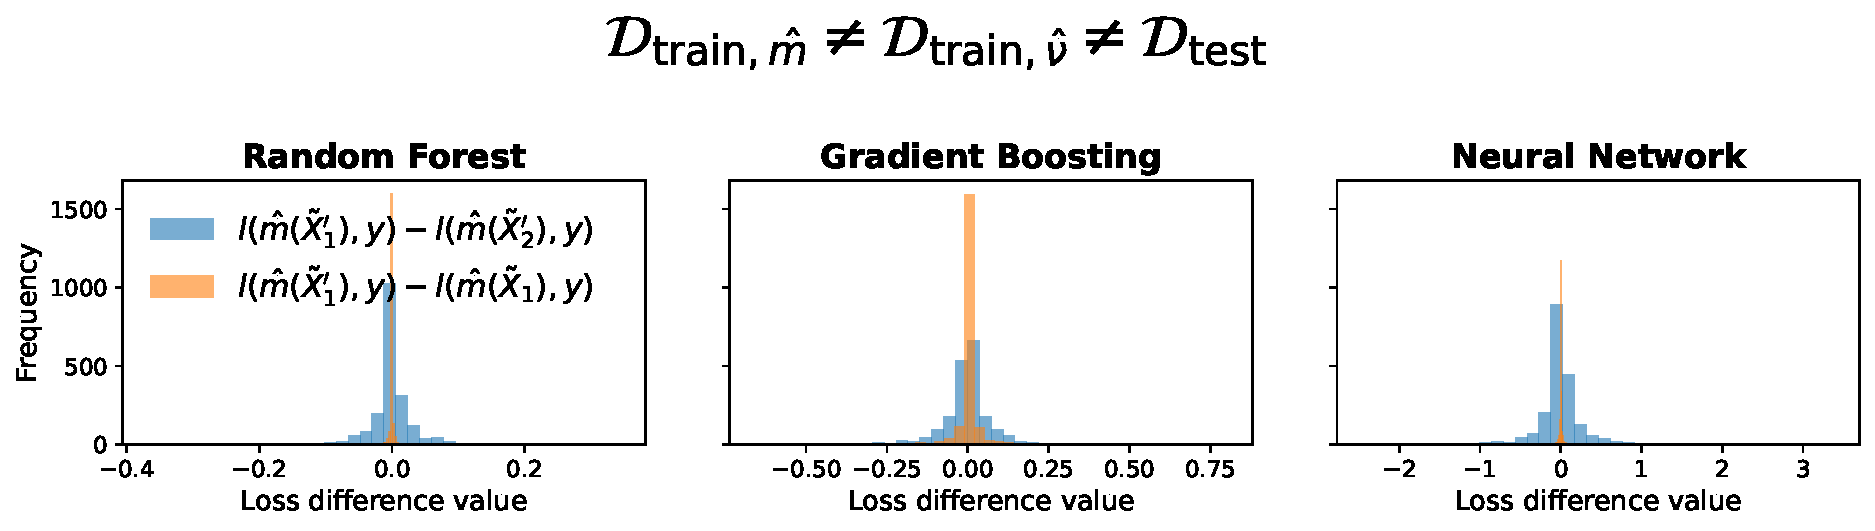
\includegraphics[width=0.7\textwidth]{images/DR/DR_sep_D.pdf}
    \caption{\textbf{Double Robustness:} Distribution of the semi-knockoff statistic, i.e., at two independently sampled estimated residuals (blue: $l(\widehat{m}(\widetilde{X}_1'), y) - l(\widehat{m}(\widetilde{X}_2'), y)$), and distribution of the difference between the theoretical and estimated residuals (orange: $l(\widehat{m}(\widetilde{X}_1'), y) - l(\widehat{m}(\widetilde{X}_1), y)$) for a null coordinate ($j=0$). The data-generating model is $y = 0.8X^1 + 0.6X^2 + 0.4X^3 + 0.2X^4 + \sin(X^1) + \epsilon$, with $\epsilon \sim \mathcal{N}(0, 0.5)$. We use $n = 2000$ samples with $X \sim \mathcal{N}(0, \Sigma)$, where $\Sigma^{i,j} = 0.5^{|i-j|}$. We use an independent test set and independent train set for each model.
 }
    \label{fig:DR_sep_D}
\end{figure}


\begin{figure}
    \centering
    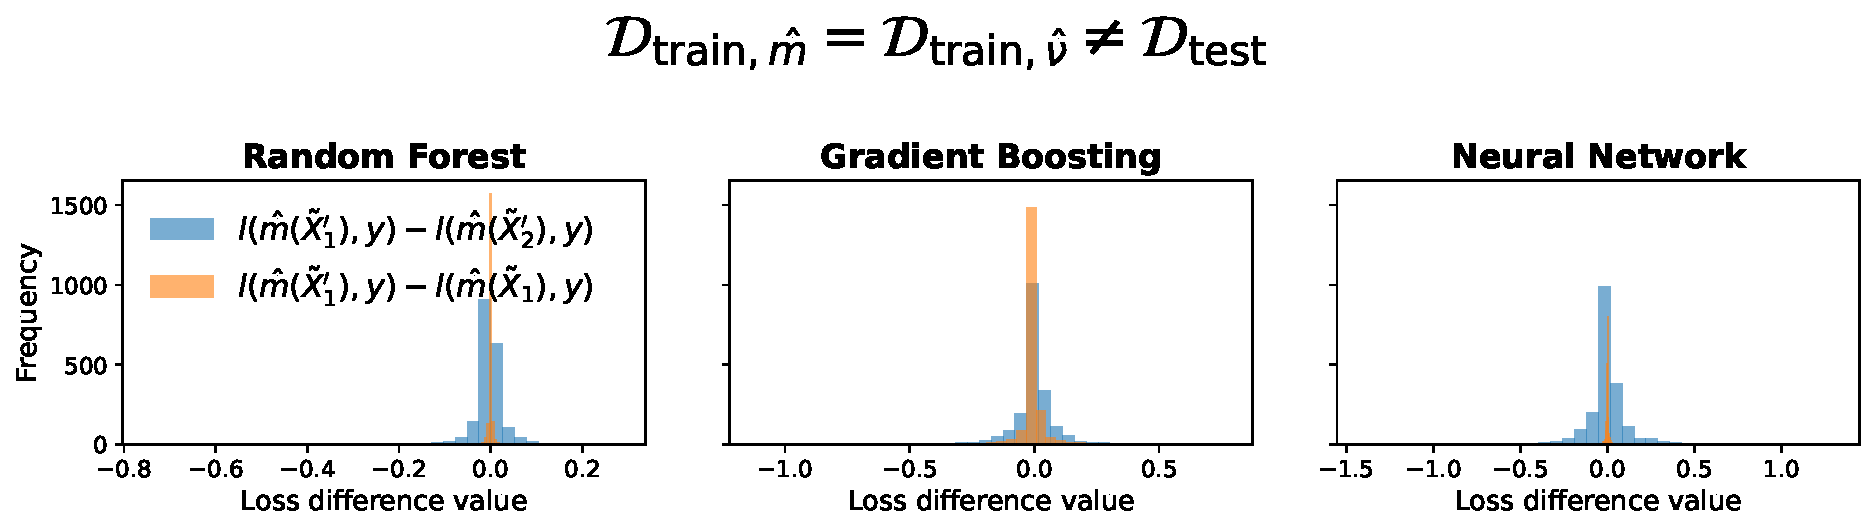
\includegraphics[width=0.7\textwidth]{images/DR/DR_med_D.pdf}
    \caption{\textbf{Double Robustness:} Distribution of the semi-knockoff statistic, i.e., the difference in loss evaluated at two independently sampled estimated residuals (blue: $l(\widehat{m}(\widetilde{X}_1'), y) - l(\widehat{m}(\widetilde{X}_2'), y)$), and distribution of the difference between the theoretical and estimated residuals (orange: $l(\widehat{m}(\widetilde{X}_1'), y) - l(\widehat{m}(\widetilde{X}_1), y)$) for a null coordinate ($j=0$). The data-generating model is $y = 0.8X^1 + 0.6X^2 + 0.4X^3 + 0.2X^4 + \sin(X^1) + \epsilon$, with $\epsilon \sim \mathcal{N}(0, 0.5)$. We use $n = 2000$ samples with $X \sim \mathcal{N}(0, \Sigma)$, where $\Sigma^{i,j} = 0.5^{|i-j|}$. We use an independent test set and the same train set for each model.
 }
    \label{fig:DR_med_D}
\end{figure}



\begin{figure}
    \centering
    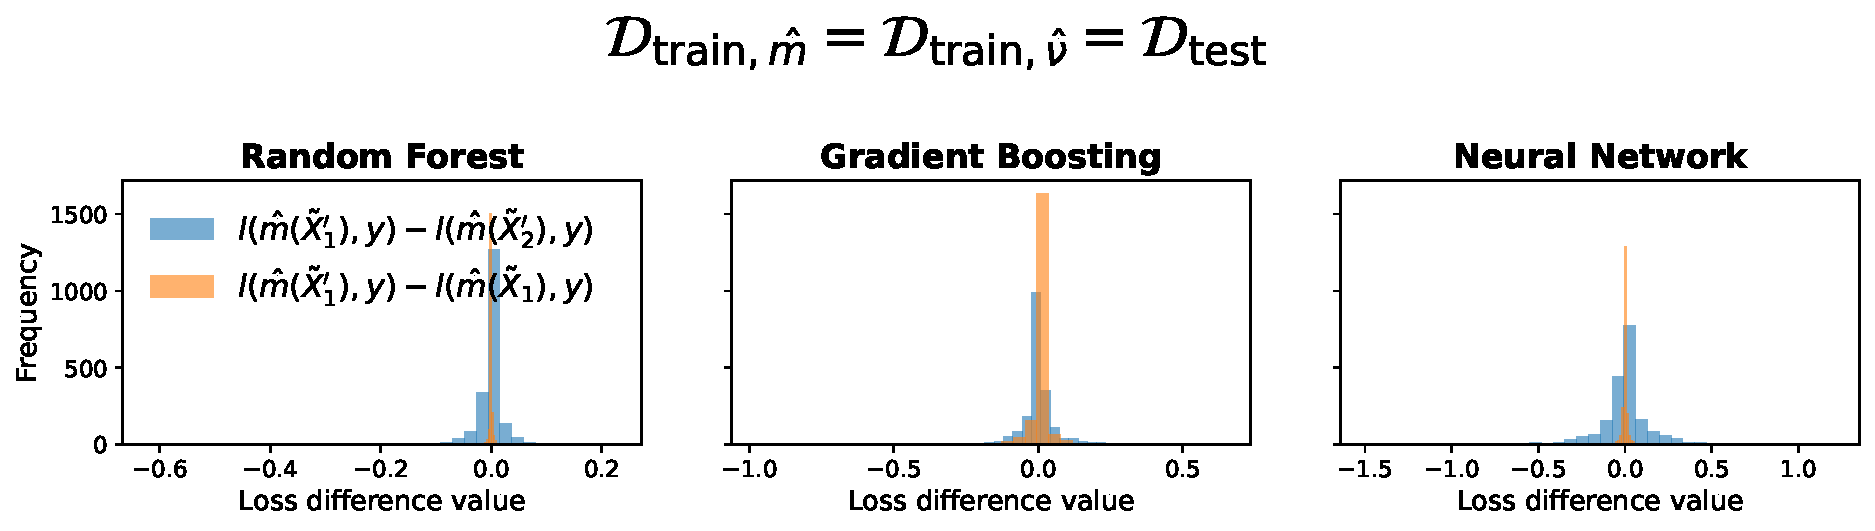
\includegraphics[width=0.7\textwidth]{images/DR/DR_unique_D.pdf}
    \caption{\textbf{Double Robustness:} Distribution of the semi-knockoff statistic, i.e., the difference in loss evaluated at two independently sampled estimated residuals (blue: $l(\widehat{m}(\widetilde{X}_1'), y) - l(\widehat{m}(\widetilde{X}_2'), y)$), and distribution of the difference between the theoretical and estimated residuals (orange: $l(\widehat{m}(\widetilde{X}_1'), y) - l(\widehat{m}(\widetilde{X}_1), y)$) for a null coordinate ($j=0$). The data-generating model is $y = 0.8X^1 + 0.6X^2 + 0.4X^3 + 0.2X^4 + \sin(X^1) + \epsilon$, with $\epsilon \sim \mathcal{N}(0, 0.5)$. We use $n = 2000$ samples with $X \sim \mathcal{N}(0, \Sigma)$, where $\Sigma^{i,j} = 0.5^{|i-j|}$. We use a unique test and train set.
 }
    \label{fig:DR_unique}
\end{figure}


Finally, in Figures~\ref{fig:DR_lin_sep} and \ref{fig:DR_lin_unique}, we study the same property in a higher-dimensional setting and include additional models. We observe that the double robustness phenomenon persists, as indicated by the orange distribution being more concentrated around zero, and that exchangeability still holds in practice, since the blue distribution remains approximately symmetric around zero.


\begin{figure}
    \centering
    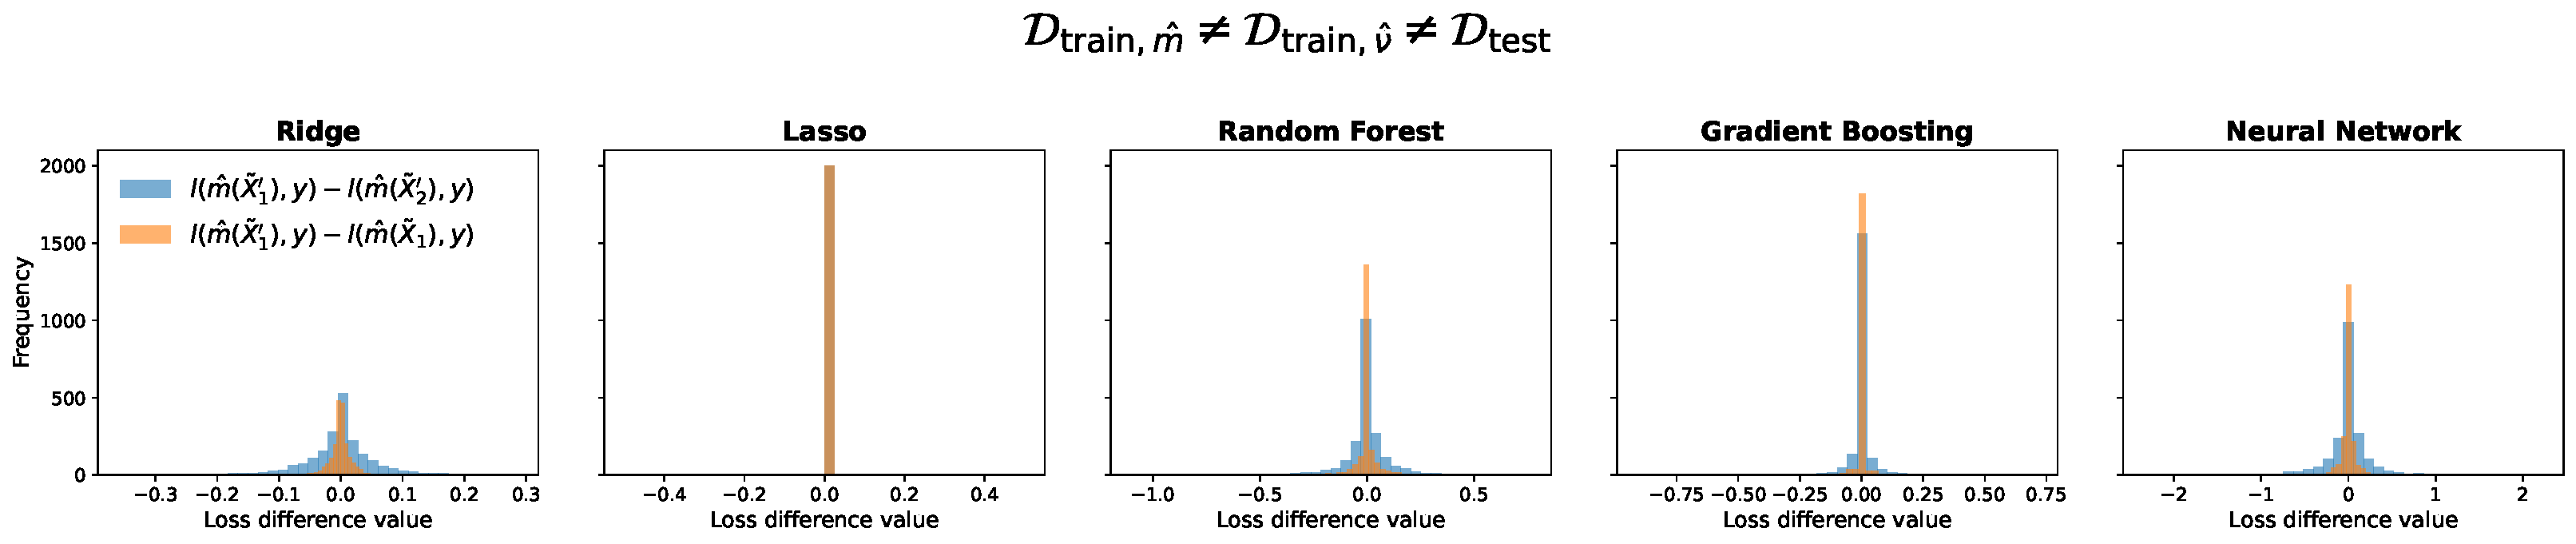
\includegraphics[width=1.02\textwidth]{images/DR/DR_highdim_sep_linear.pdf}
    \caption{\textbf{Double Robustness:} Distribution of the semi-knockoff statistic, i.e., the difference in loss evaluated at two independently sampled estimated residuals (blue: $l(\widehat{m}(\widetilde{X}_1'), y) - l(\widehat{m}(\widetilde{X}_2'), y)$), and distribution of the difference between the theoretical and estimated residuals (orange: $l(\widehat{m}(\widetilde{X}_1'), y) - l(\widehat{m}(\widetilde{X}_1), y)$) for a null coordinate ($j=0$). The data-generating model is $y = X^\top \beta + \epsilon$, with $\epsilon \sim \mathcal{N}(0, 0.5)$ and $\beta$ $0.5$-sparse randomly sampled with half of the values equally sampled from $0.3$ to $1$, and the other half from $-0.8$ to $-0.2$. We use $n_{\mathrm{train}, ,\widehat{m} }= 500$ samples for training $\widehat{m}$ and $n_{\mathrm{train} ,\widehat{\nu}}=n_\mathrm{test}=2000$ for training $\widehat{\nu}$ and $\widehat{\rho}$ with $X \sim \mathcal{N}(0, \Sigma)$, where $\Sigma^{i,j} = 0.5^{|i-j|}$ and $X\in \mathbb{R}^{50}$. We use an independent test set and independent train set for each model. 
 }
    \label{fig:DR_lin_sep}
\end{figure}


\begin{figure}
    \centering
    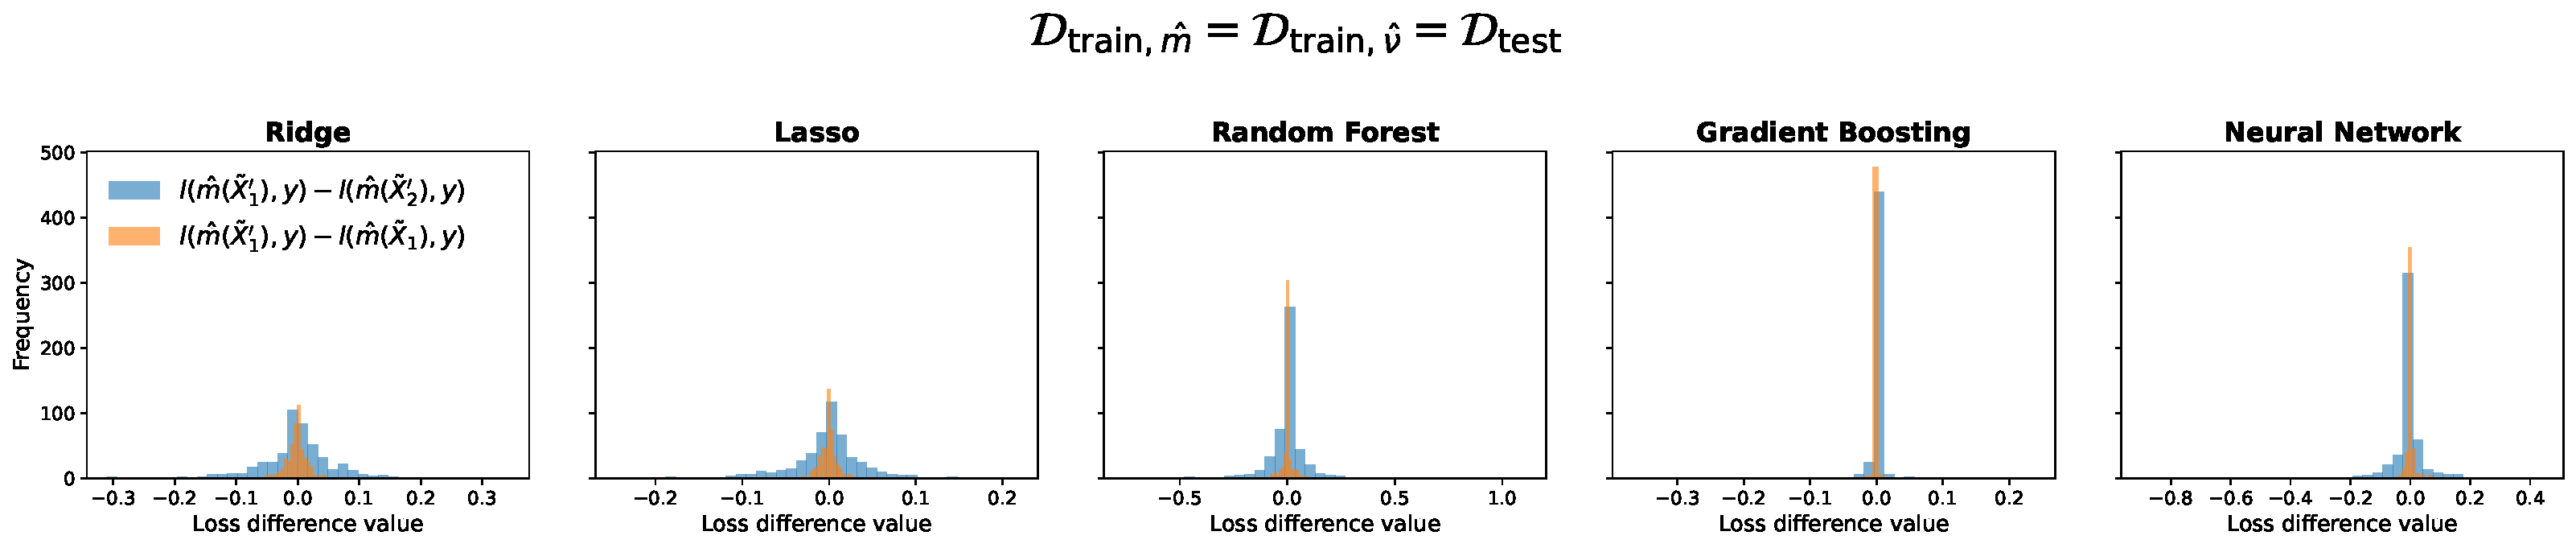
\includegraphics[width=1.02\textwidth]{images/DR/DR_highdim_complex_linear.pdf}
    \caption{\textbf{Double Robustness:} Distribution of the semi-knockoff statistic, i.e., the difference in loss evaluated at two independently sampled estimated residuals (blue: $l(\widehat{m}(\widetilde{X}_1'), y) - l(\widehat{m}(\widetilde{X}_2'), y)$), and distribution of the difference between the theoretical and estimated residuals (orange: $l(\widehat{m}(\widetilde{X}_1'), y) - l(\widehat{m}(\widetilde{X}_1), y)$) for a null coordinate ($j=0$). The data-generating model is $y = X^\top \beta + \epsilon$, with $\epsilon \sim \mathcal{N}(0, 0.5)$ and $\beta$ $0.5$-sparse randomly sampled with half of the values equally sampled from $0.3$ to $1$, and the other half from $-0.8$ to $-0.2$. We use $n = 500$ samples with $X \sim \mathcal{N}(0, \Sigma)$, where $\Sigma^{i,j} = 0.5^{|i-j|}$ and $X\in \mathbb{R}^{50}$. We use a unique test and train set.
 }
    \label{fig:DR_lin_unique}
\end{figure}



\subsection{Exchangeability}

In Figure~\ref{fig:fdp_illustration}, we observe that, in practice, the sampling scheme effectively preserves the required symmetry under the null. This exchangeability (Lemma~\ref{lemma:exchang}) lies at the heart of knockoff FDR control, since the threshold estimates the number of false discoveries by exploiting this symmetry. This is reflected by the distribution of the null features (blue dots), which is approximately symmetric around 0. As a result, the knockoff threshold successfully controls the FDR across standard ML models, such as Lasso, Ridge, Gradient Boosting, Random Forest, and Neural Networks. Moreover, the important features exhibit a distribution that is clearly separated from that of the nulls, yielding a powerful testing procedure that consists of selecting the coordinates whose statistics are above the threshold (red line).


\begin{figure}
    \centering
    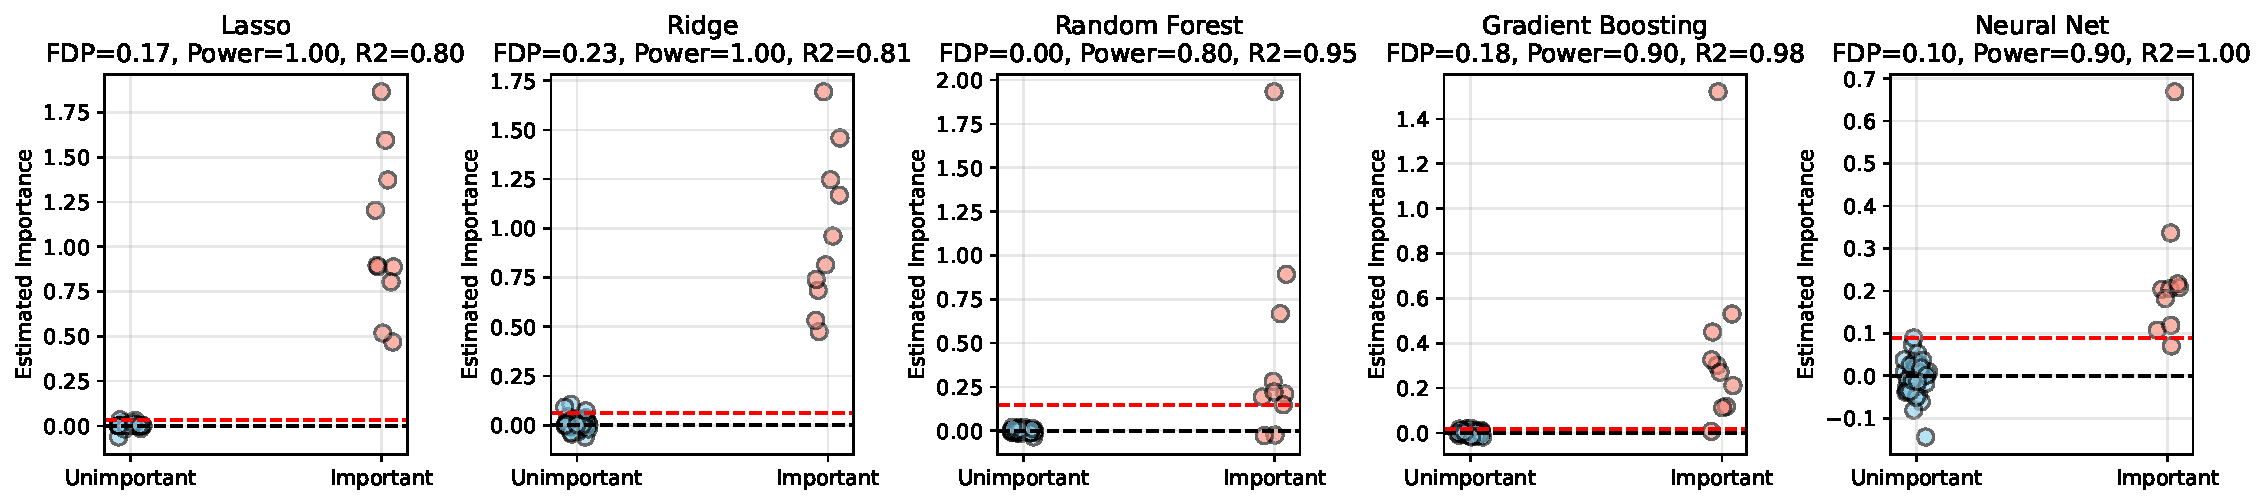
\includegraphics[width=1.05\textwidth]{images/new_exp/fdp_illustration.pdf}
    \caption{\textbf{Semi-knockoff statistics:} $y = X\beta + \epsilon$, where $\beta$ is 0.25-sparse with important features grouped in blocks of 5 sampled uniformly. The noise level is $\|X\beta\|/2$. The design matrix satisfies $X \sim \mathcal{N}(0, \Sigma)$ with $\Sigma_{i,j} = 0.6^{|i-j|}$. We set $n = 300$ and $p = 50$. The figure displays the distribution of the Semi-knockoff statistics for several standard ML models. In each plot, the null features are shown on the left and the important features on the right. The red horizontal line denotes the data-dependent knockoff threshold corresponding to a target FDR level of $q = 0.2$.
 }
    \label{fig:fdp_illustration}
\end{figure}



\subsection{Type-I error}

In this section, we present the type-I error control experiments using the settings from the main text across several models: the adjacent support setting from Figure~\ref{fig:main_adj_gb} and the masked correlation setting from Figure~\ref{fig:main_masked_nn}. Our goal is to verify that the observed behavior remains consistent for standard ML models, namely neural networks, gradient boosting, and random forests. All models were implemented using \texttt{scikit-learn}~\cite{scikit-learn}. We recall that across the experiments $n=300$ and $p=50$. We additionally include an analysis of computation time.

\paragraph{Computation time.}
Semi-knockoffs are expected to offer substantial computational improvements relative to other CIT methods such as LOCO, dCRT, and HRT. In our experiments, we used multiple models with default hyperparameters, so the differences were somewhat muted for complex models. However, LOCO and the distillation step of dCRT require re-fitting a complex model for each feature. Moreover, both dCRT and HRT require resampling the data thousands of times to compute each p-value. In contrast, Semi-knockoffs can be optimized to avoid these repeated refits and resampling steps, and therefore have the potential to be significantly faster in practice.

 

\subsubsection{Adjacent support}


This setting consists of having an adjacent support, such that all important features ($0.25p$) form a contiguous block. The results were similar with a randomly sampled support. The main observations from Figure~\ref{fig:main_adj_gb} are: (i) the low power of VIM, which highlights the need for a CIT procedure compatible with arbitrary pre-trained models; and (ii) the reduced power of HRT due to the data-splitting step, relative to Semi-knockoffs. These conclusions are consistent with Figures~\ref{fig:app_adj_nn}, \ref{fig:app_adj_gb}, and \ref{fig:app_adj_rf}, corresponding to neural networks, gradient boosting, and random forests, respectively. The only exception is the neural network case, where the model attains high predictive accuracy even under data splitting ($R^2 = 0.963$), resulting in HRT exhibiting full power and therefore not lagging behind methods that avoid data splitting ($R^2 = 0.965$). For the other models, we observe a clear gain from avoiding the data-splitting step.

Overall, all methods control the type-I error except \texttt{LOCO-W}~\cite{williamson2023general}, which provides only asymptotic type-I error guarantees and requires an additional train–train split for the original and restricted models; in practice, it fails to control the type-I error and also incurs a loss in power. We also note that, similarly to the power, the AUC for \texttt{dCRT} and \texttt{Semi-knockoffs} outperforms the other methods, and that a 5-permutation derandomization step can be beneficial for power.


\begin{figure}
    \centering
    
\includegraphics[width=1.03\textwidth]{images/experiments_p_val/adjacent_NN.pdf}
    \caption{\textbf{Type-I error adjacent support with Neural Network.} Let $X \sim \mathcal{N}(0,\Sigma)$ with $\Sigma^{ij} = 0.6^{|i-j|}$, and $y = \beta^\top X + \epsilon$, where the first $0.25p$ coordinates of $\beta$ are between $1$ and $2$ and the remaining entries are zero, and $\epsilon \sim \mathcal{N}(0,1)$. The black-box pretrained model $\widehat{m}$ is a neural network.
    }
    \label{fig:app_adj_nn}
\end{figure}



\begin{figure}
    \centering
    
\includegraphics[width=1.03\textwidth]{images/experiments_p_val/adjacent_GB.pdf}
    \caption{\textbf{Type-I error adjacent support with Gradient Boosting.} Let $X \sim \mathcal{N}(0,\Sigma)$ with $\Sigma^{ij} = 0.6^{|i-j|}$, and $y = \beta^\top X + \epsilon$, where the first $0.25p$ coordinates of $\beta$ are between $1$ and $2$ and the remaining entries are zero, and $\epsilon \sim \mathcal{N}(0,1)$. The black-box pretrained model $\widehat{m}$ is a gradient boosting. }
    \label{fig:app_adj_gb}
\end{figure}


\begin{figure}
    \centering
    
\includegraphics[width=1.03\textwidth]{images/experiments_p_val/adjacent_RF.pdf}
    \caption{\textbf{Type-I error adjacent support with Random Forest.} Let $X \sim \mathcal{N}(0,\Sigma)$ with $\Sigma^{ij} = 0.6^{|i-j|}$, and $y = \beta^\top X + \epsilon$, where the first $0.25p$ coordinates of $\beta$ are between $1$ and $2$ and the remaining entries are zero, and $\epsilon \sim \mathcal{N}(0,1)$. The black-box pretrained model $\widehat{m}$ is a random forest.}
    \label{fig:app_adj_rf}
\end{figure}


\subsubsection{Masked correlation}


This setting consists of a single important coordinate that is highly correlated with an unimportant feature. Under this configuration, we observe a clear gain from using a pretrained model that can evaluate the contribution of all features jointly. In contrast, the distillation step in dCRT—which consists of training a complex model between $y$ and $X^{-j}$ in order to isolate the importance of feature $X^j$ from the residual—leads to a loss of power, since the distillation shrinks the signal provided by the important feature.

The conclusions here are similar to those in the previous setting. Specifically, \texttt{Sobol-CPI} and \texttt{LOCO} (except for the Wilcoxon version) exhibit no power due to overly restrictive corrections, and there is also a noticeable loss from data splitting in \texttt{HRT}. Finally, the derandomization step increases the power of \texttt{Semi-knockoffs}.



\begin{figure}
    \centering
    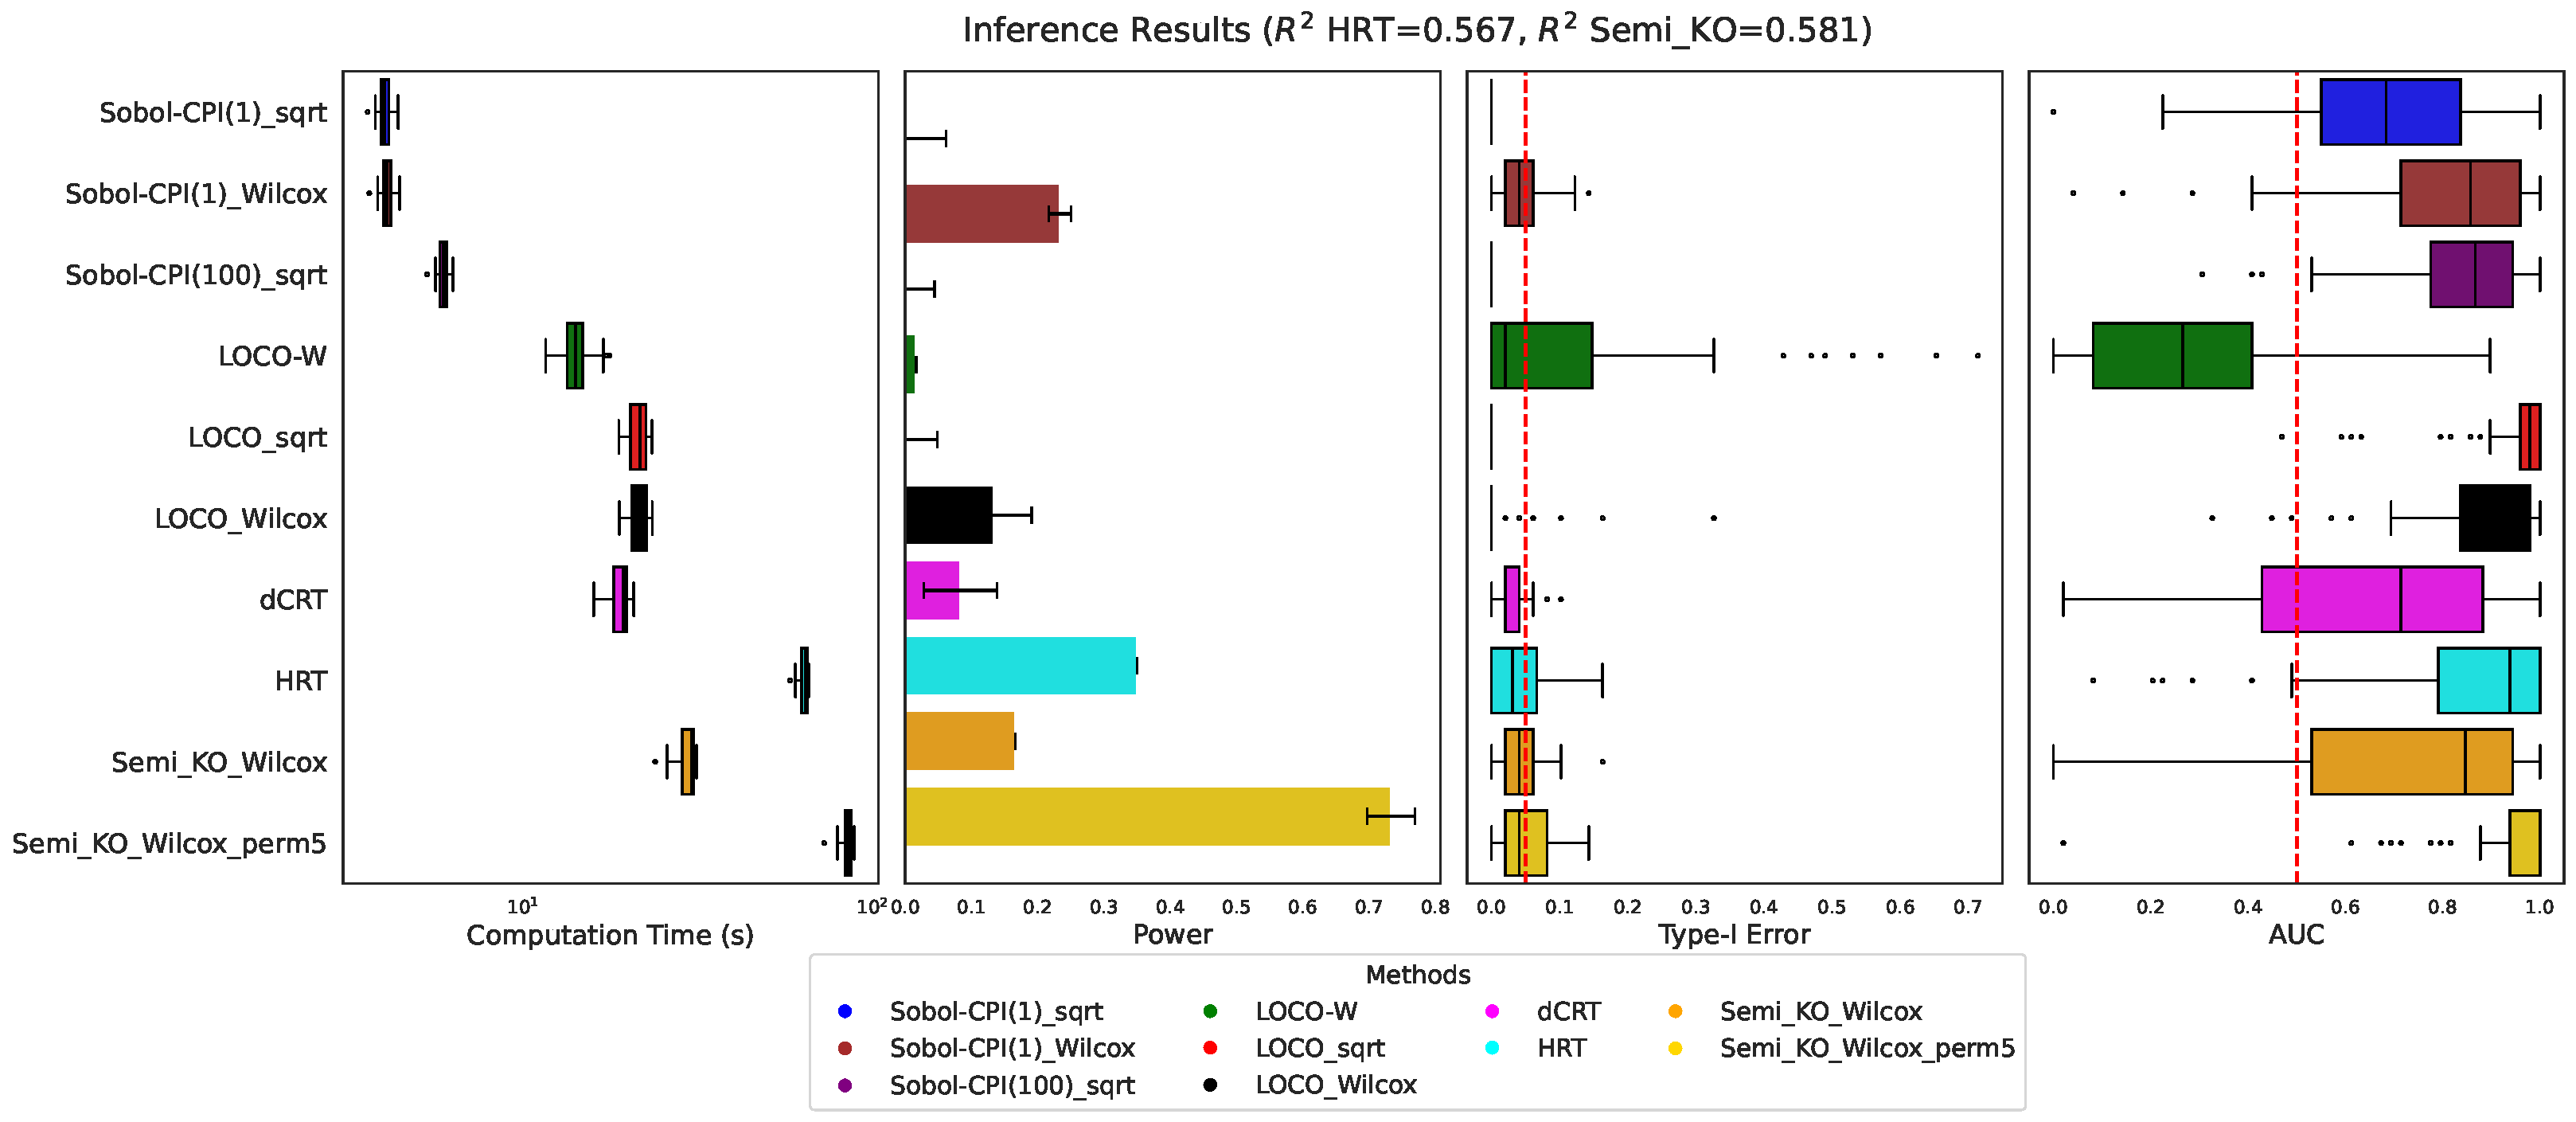
\includegraphics[width=1.03\textwidth]{images/experiments_p_val/masked_corr_NN.pdf}
    \caption{\textbf{Type-I error masked correlation with Neural Network.} Let $X \sim \mathcal{N}(0,\Sigma)$ with $\Sigma_{ij} = 0.6^{|i-j|}$. A unique relevant coordinate $l$ is sampled and $y = X_l + 0.5\,\epsilon_1$, where $\epsilon_1 \sim \mathcal{N}(0,1)$. A correlated null variable is created as $X_{l-1} = X_l + 0.5\,\epsilon_2$, with $\epsilon_2 \sim \mathcal{N}(0,1)$. The black-box pretrained model $\widehat{m}$ is a neural network.
 }
    \label{fig:app_masked_nn}
\end{figure}



\begin{figure}
    \centering
    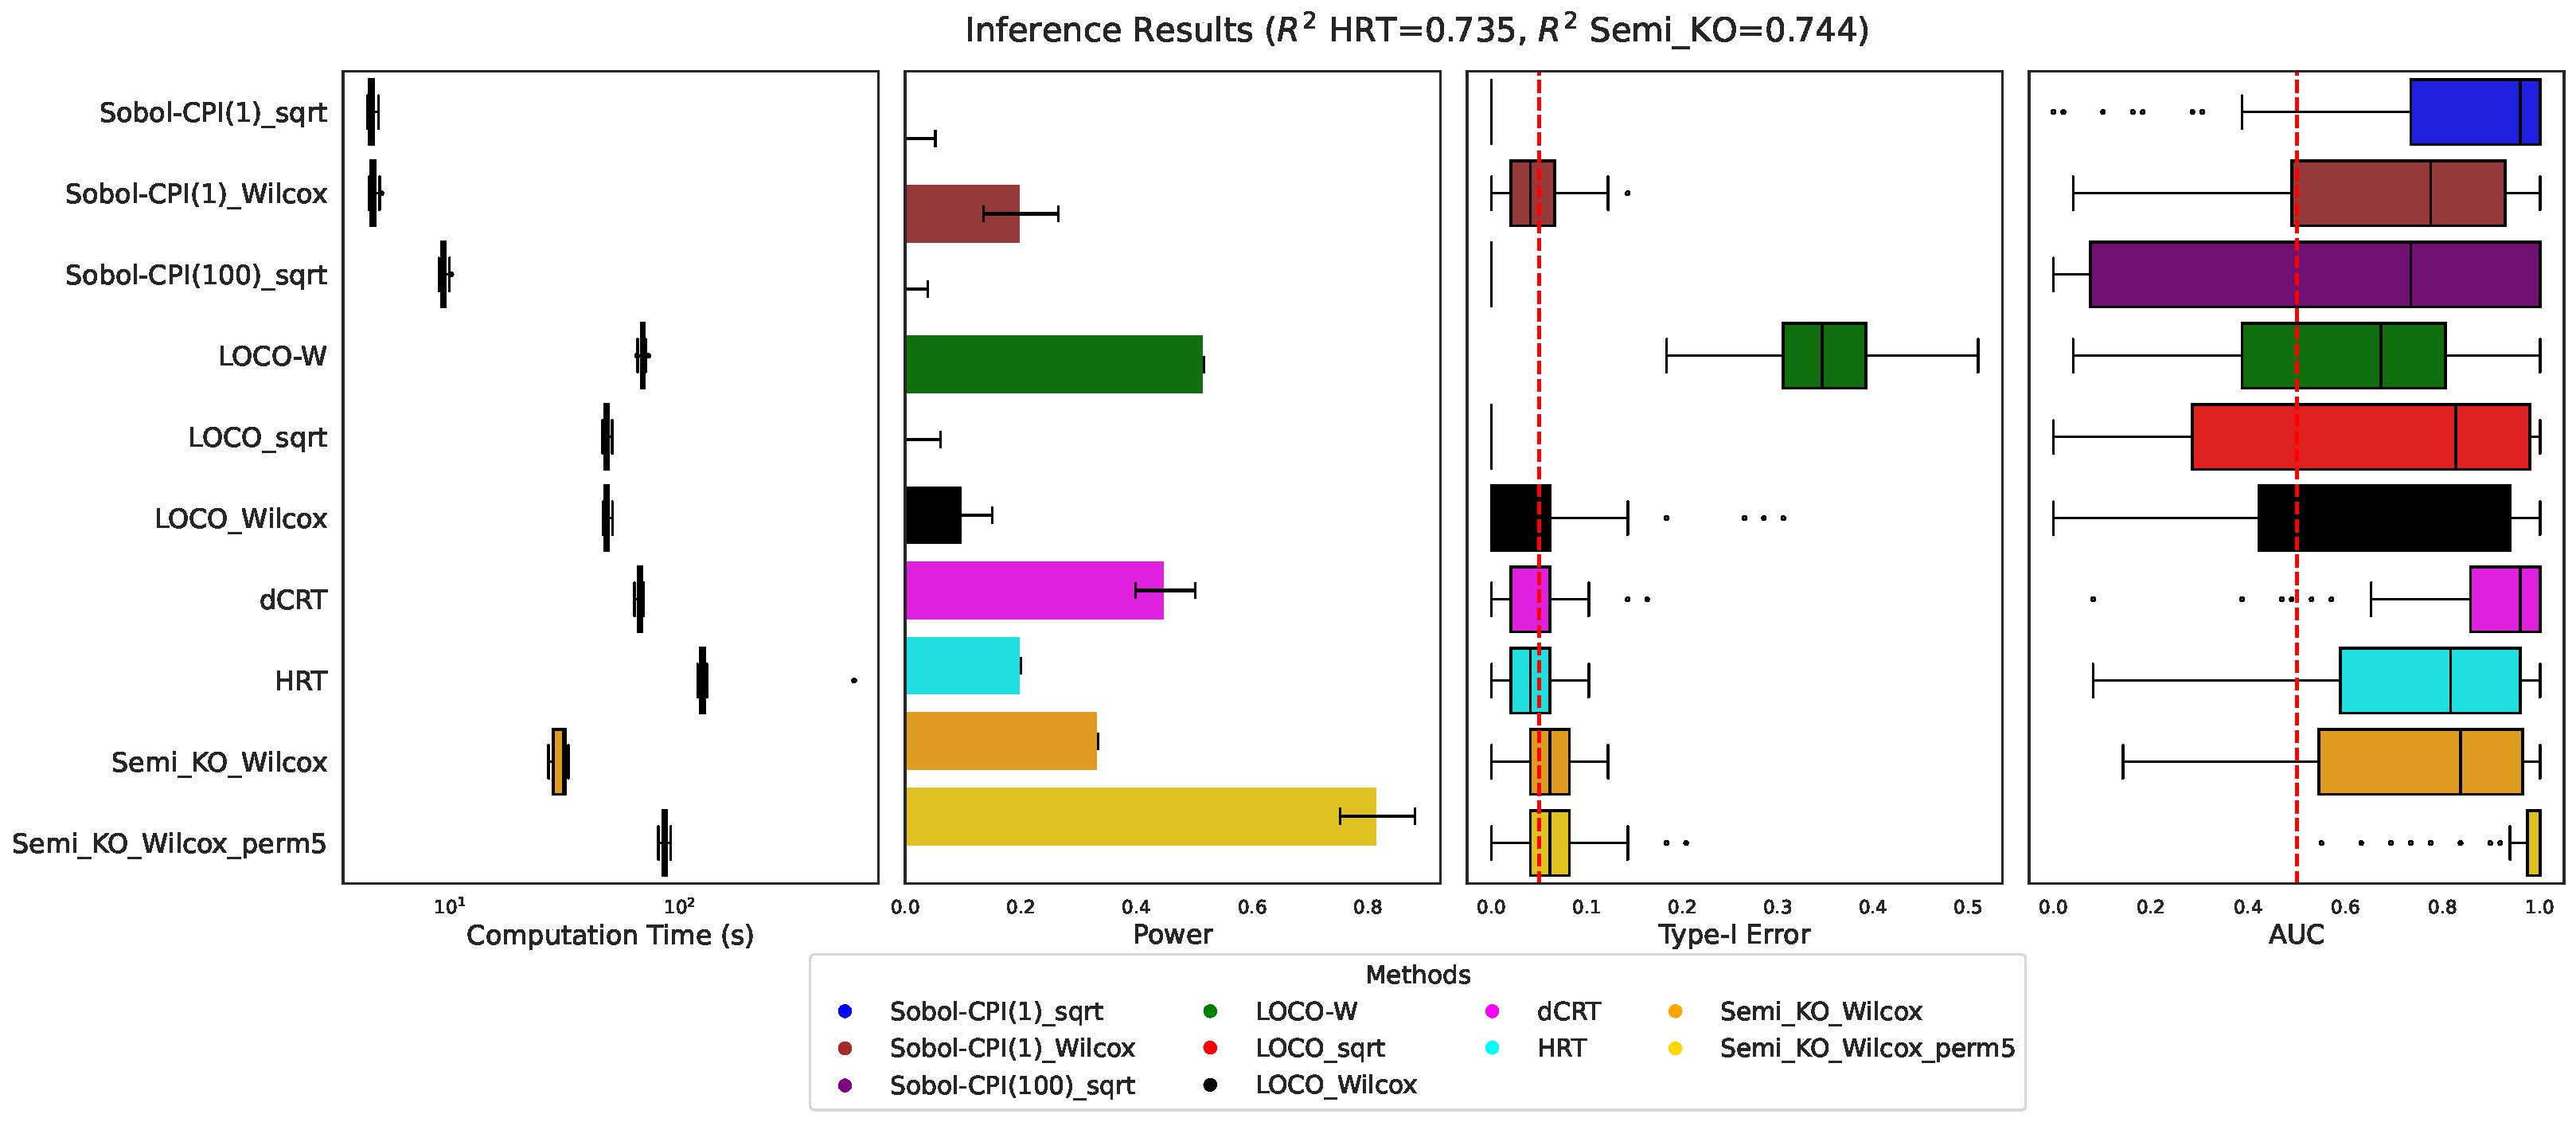
\includegraphics[width=1.03\textwidth]{images/experiments_p_val/masked_corr_GB.pdf}
    \caption{\textbf{Type-I error masked correlation with Gradient Boosting.} Let $X \sim \mathcal{N}(0,\Sigma)$ with $\Sigma_{ij} = 0.6^{|i-j|}$. A unique relevant coordinate $l$ is sampled and $y = X_l + 0.5\,\epsilon_1$, where $\epsilon_1 \sim \mathcal{N}(0,1)$. A correlated null variable is created as $X_{l-1} = X_l + 0.5\,\epsilon_2$, with $\epsilon_2 \sim \mathcal{N}(0,1)$. The black-box pretrained model $\widehat{m}$ is a gradient boosting.
 }
    \label{fig:app_masked_GB}
\end{figure}



\begin{figure}
    \centering
    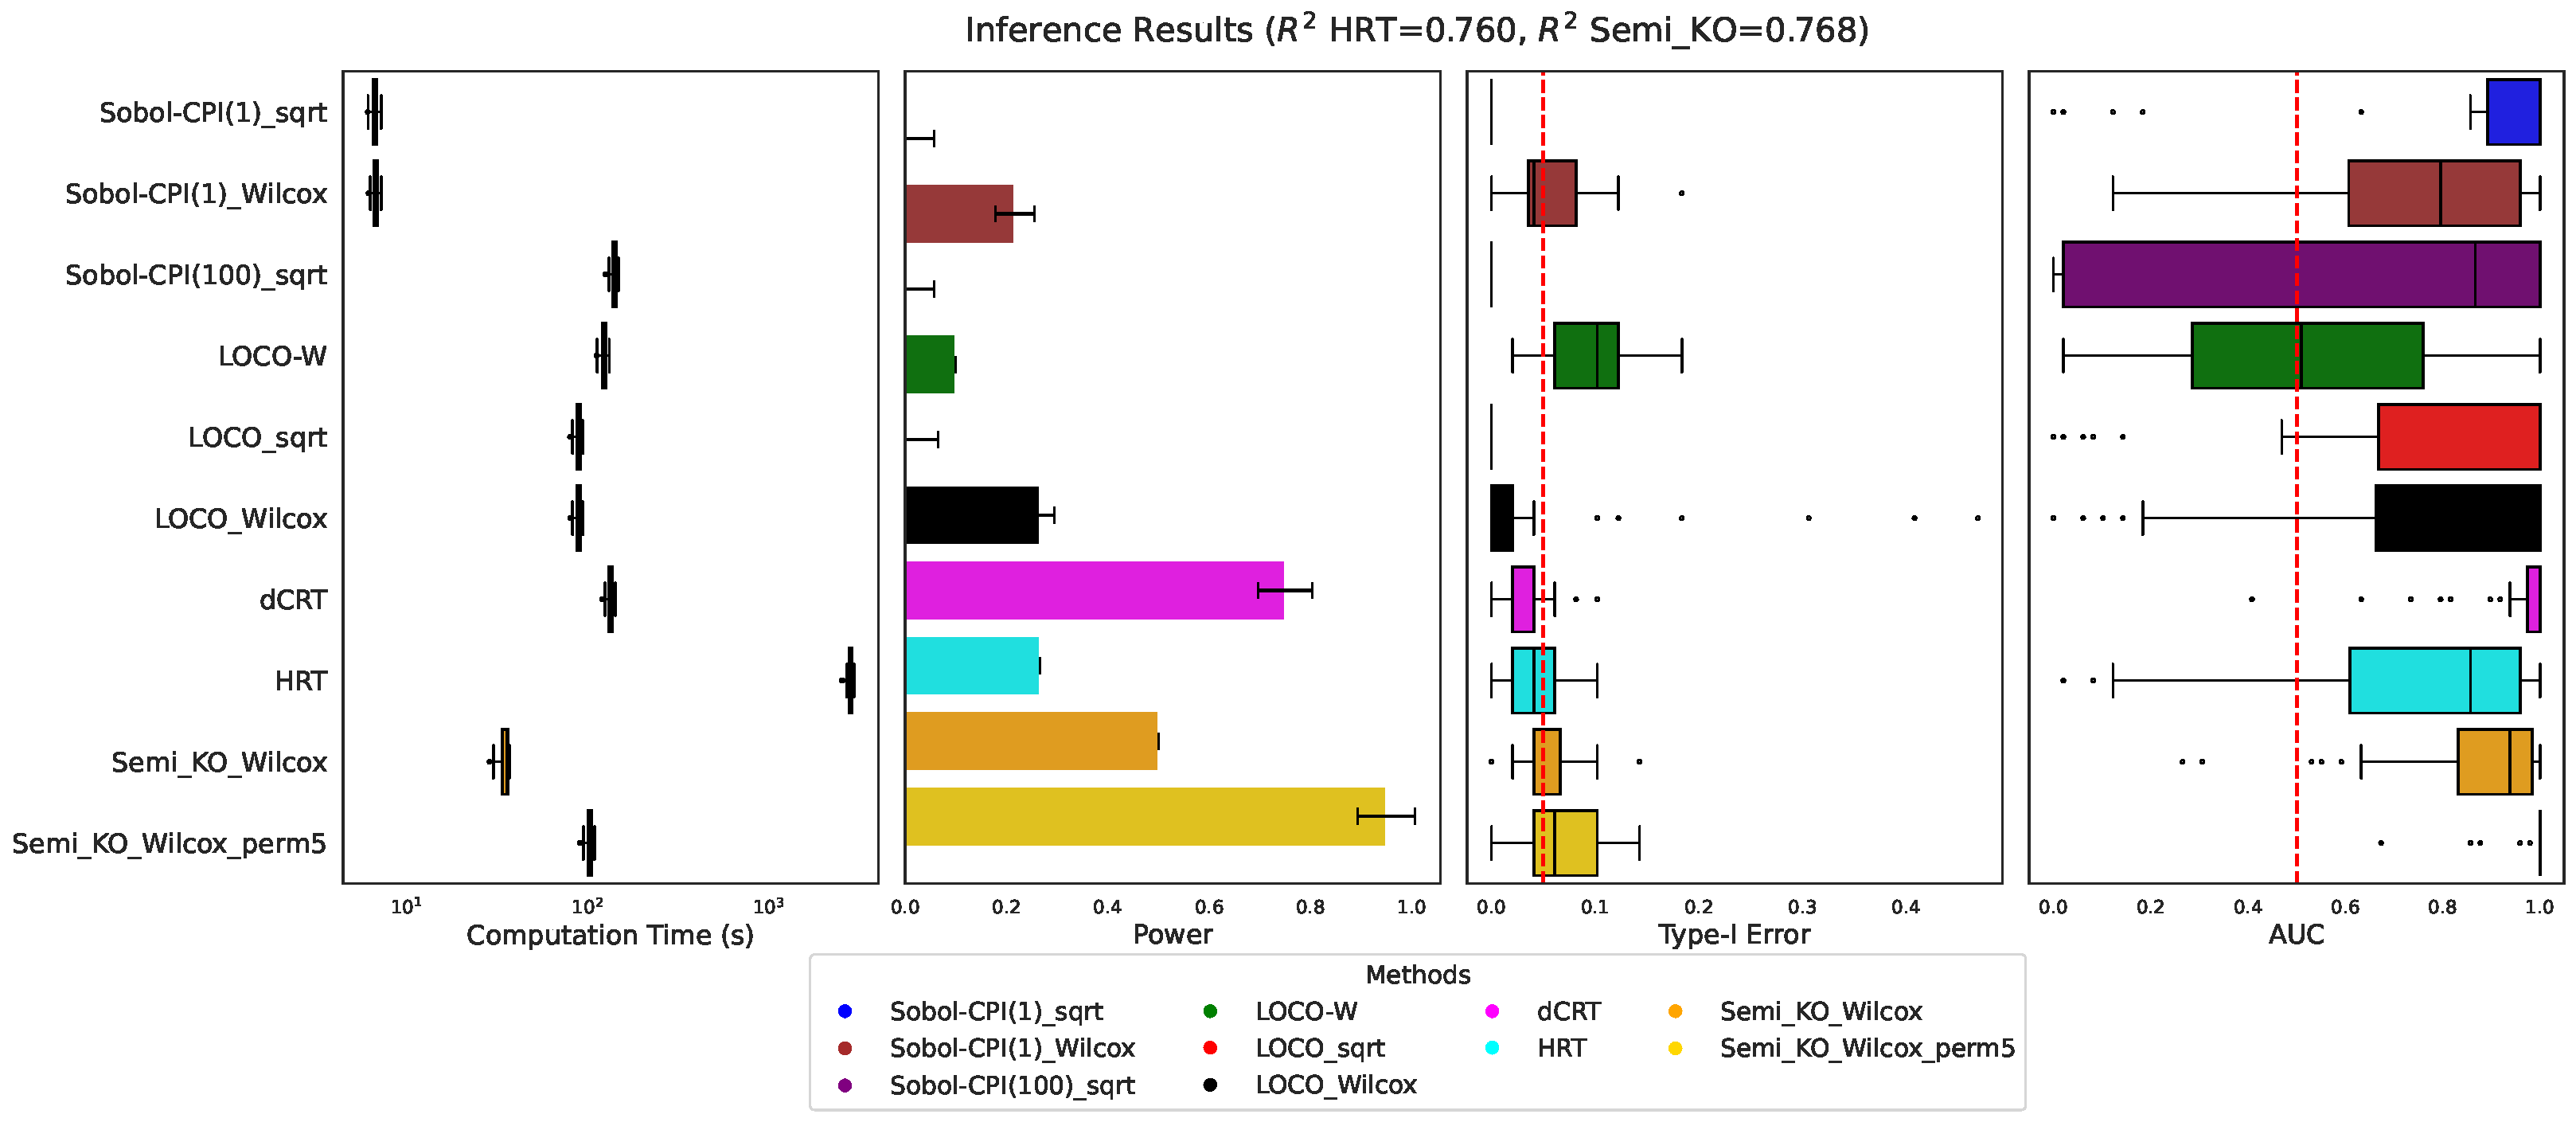
\includegraphics[width=1.03\textwidth]{images/experiments_p_val/masked_corr_RF.pdf}
    \caption{\textbf{Type-I error masked correlation with Random Forest.} Let $X \sim \mathcal{N}(0,\Sigma)$ with $\Sigma_{ij} = 0.6^{|i-j|}$. A unique relevant coordinate $l$ is sampled and $y = X_l + 0.5\,\epsilon_1$, where $\epsilon_1 \sim \mathcal{N}(0,1)$. A correlated null variable is created as $X_{l-1} = X_l + 0.5\,\epsilon_2$, with $\epsilon_2 \sim \mathcal{N}(0,1)$. The black-box pretrained model $\widehat{m}$ is a random forest.
 }
    \label{fig:app_masked_RF}
\end{figure}


\subsection{False Discovery Rate}\label{app:fdr_exp}


In this section, we provide additional intuition regarding the FDR control experiments for Semi-knockoffs. All previously discussed procedures that produce valid p-values can be adapted to FDR control by applying a multiple-testing correction procedure such as BH~\cite{BH}. However, such guarantees are not exact, since the dependence structure among the p-values is unknown, and may violate the assumptions under which BH ensures FDR control. 

In contrast, procedures such as standard \texttt{Knockoffs} and \texttt{Semi-knockoffs} provide exact FDR control by construction. In principle, the Semi-knockoffs framework could be adapted either by applying BH to the p-values from the Wilcoxon version, or by directly applying the knockoff threshold to control the FDR. As our experiments indicate, the latter strategy should be preferred in practice and in theory.

We present results for the Adjacent setting from the previous section, but now focusing on FDR control, as well as for a heavy-tailed setting. These experiments are conducted using neural network, gradient boosting, and random forest models.

\subsubsection{Adjacent support}

We revisit the setting with a block of important features. Since the underlying model is linear, \texttt{Knockoffs} achieves high power, as expected. Moreover, we observe a similar pattern to that seen in the p-value experiments: for gradient boosting (Figure~\ref{fig:app_KO_adj_gb}) and random forest (Figure~\ref{fig:app_KO_adj_rf}), there is a clear gain from avoiding the train–test split. In particular, HRT does not attain full power, which can be attributed to the reduction in $R^2$ caused by data splitting.


\begin{figure}
    \centering
    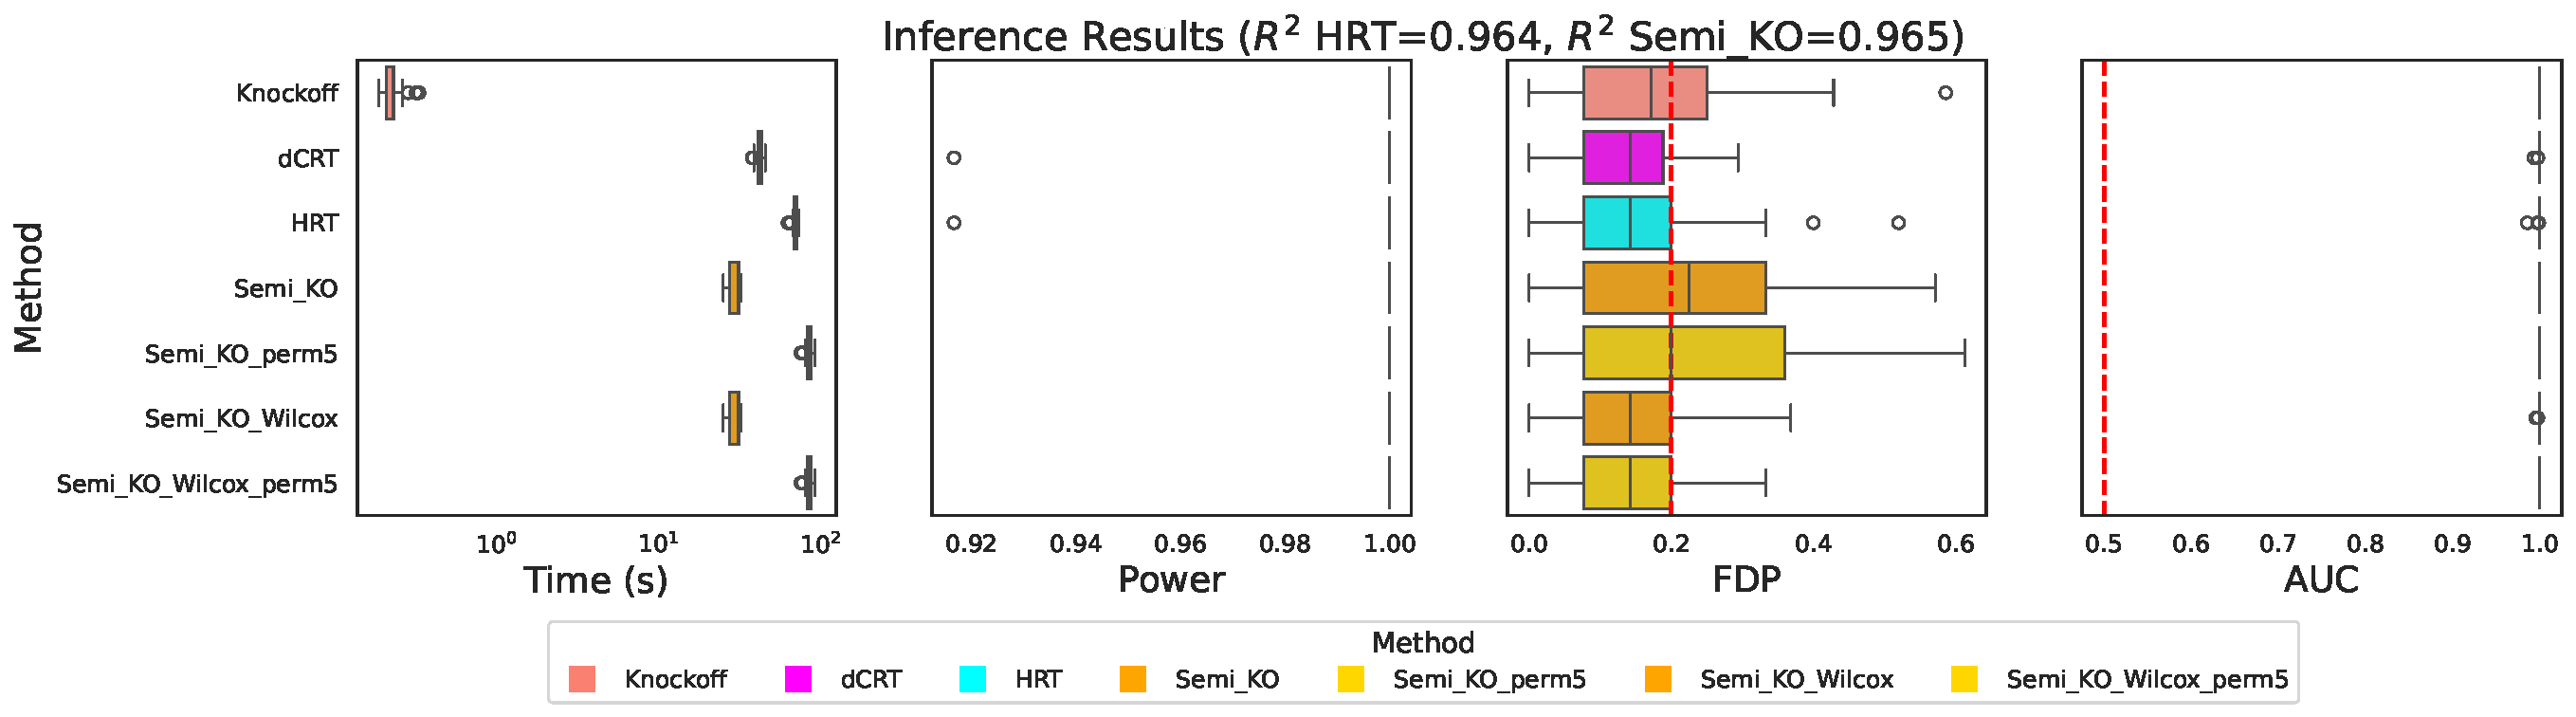
\includegraphics[width=1.03\textwidth]{images/exp_KO/adjacent_NN.pdf}
    \caption{\textbf{FDR adjacent support with Neural Network.} Let $X \sim \mathcal{N}(0,\Sigma)$ with $\Sigma^{ij} = 0.6^{|i-j|}$, and $y = \beta^\top X + \epsilon$, where the first $0.25p$ coordinates of $\beta$ are between $1$ and $2$ and the remaining entries are zero, and $\epsilon \sim \mathcal{N}(0,1)$. The black-box pretrained model $\widehat{m}$ is a neural network, achieving $R^2 = 0.964$ with a train-test split and $R^2 = 0.965$ without split.}
    \label{fig:app_KO_adj_nn}
\end{figure}


\begin{figure}
    \centering
    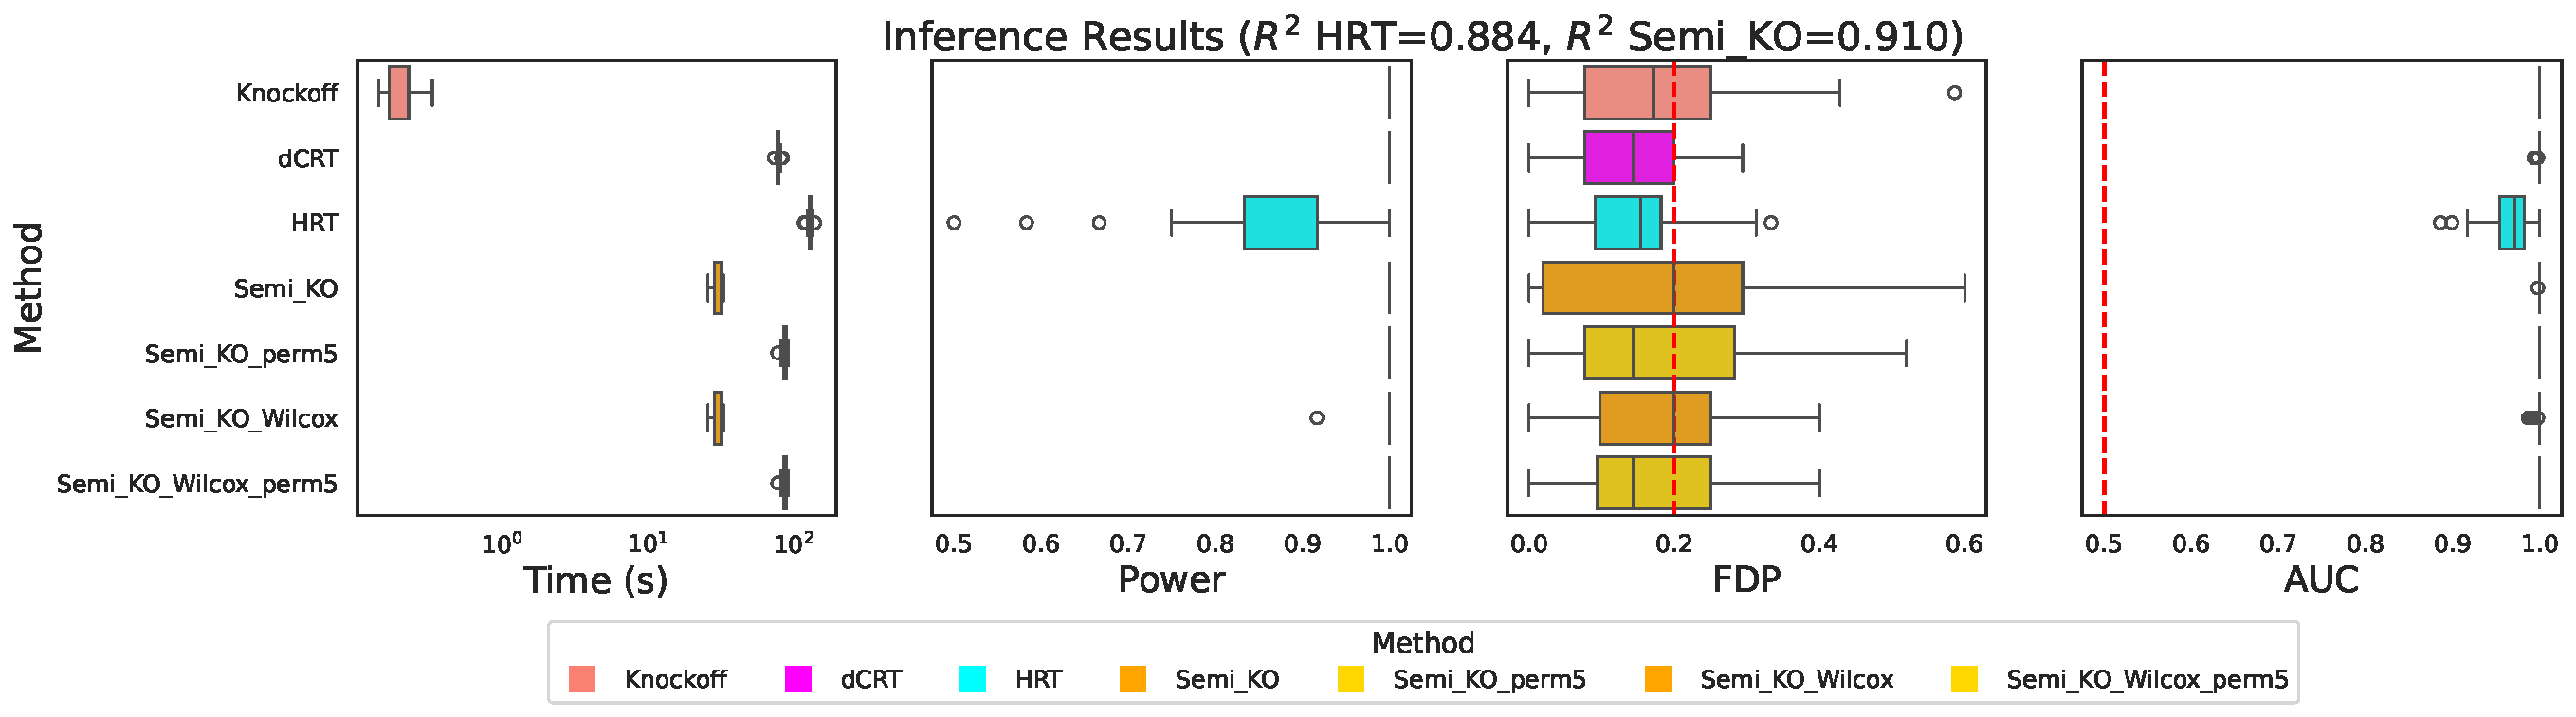
\includegraphics[width=1.03\textwidth]{images/exp_KO/adjacent_GB.pdf}
    \caption{\textbf{FDR adjacent support with Gradient Boosting.} Let $X \sim \mathcal{N}(0,\Sigma)$ with $\Sigma^{ij} = 0.6^{|i-j|}$, and $y = \beta^\top X + \epsilon$, where the first $0.25p$ coordinates of $\beta$ are between $1$ and $2$ and the remaining entries are zero, and $\epsilon \sim \mathcal{N}(0,1)$. The black-box pretrained model $\widehat{m}$ is a gradient boosting, achieving $R^2 = 0.884$ with a train-test split and $R^2 = 0.910$ without split.}
    \label{fig:app_KO_adj_gb}
\end{figure}


\begin{figure}
    \centering
    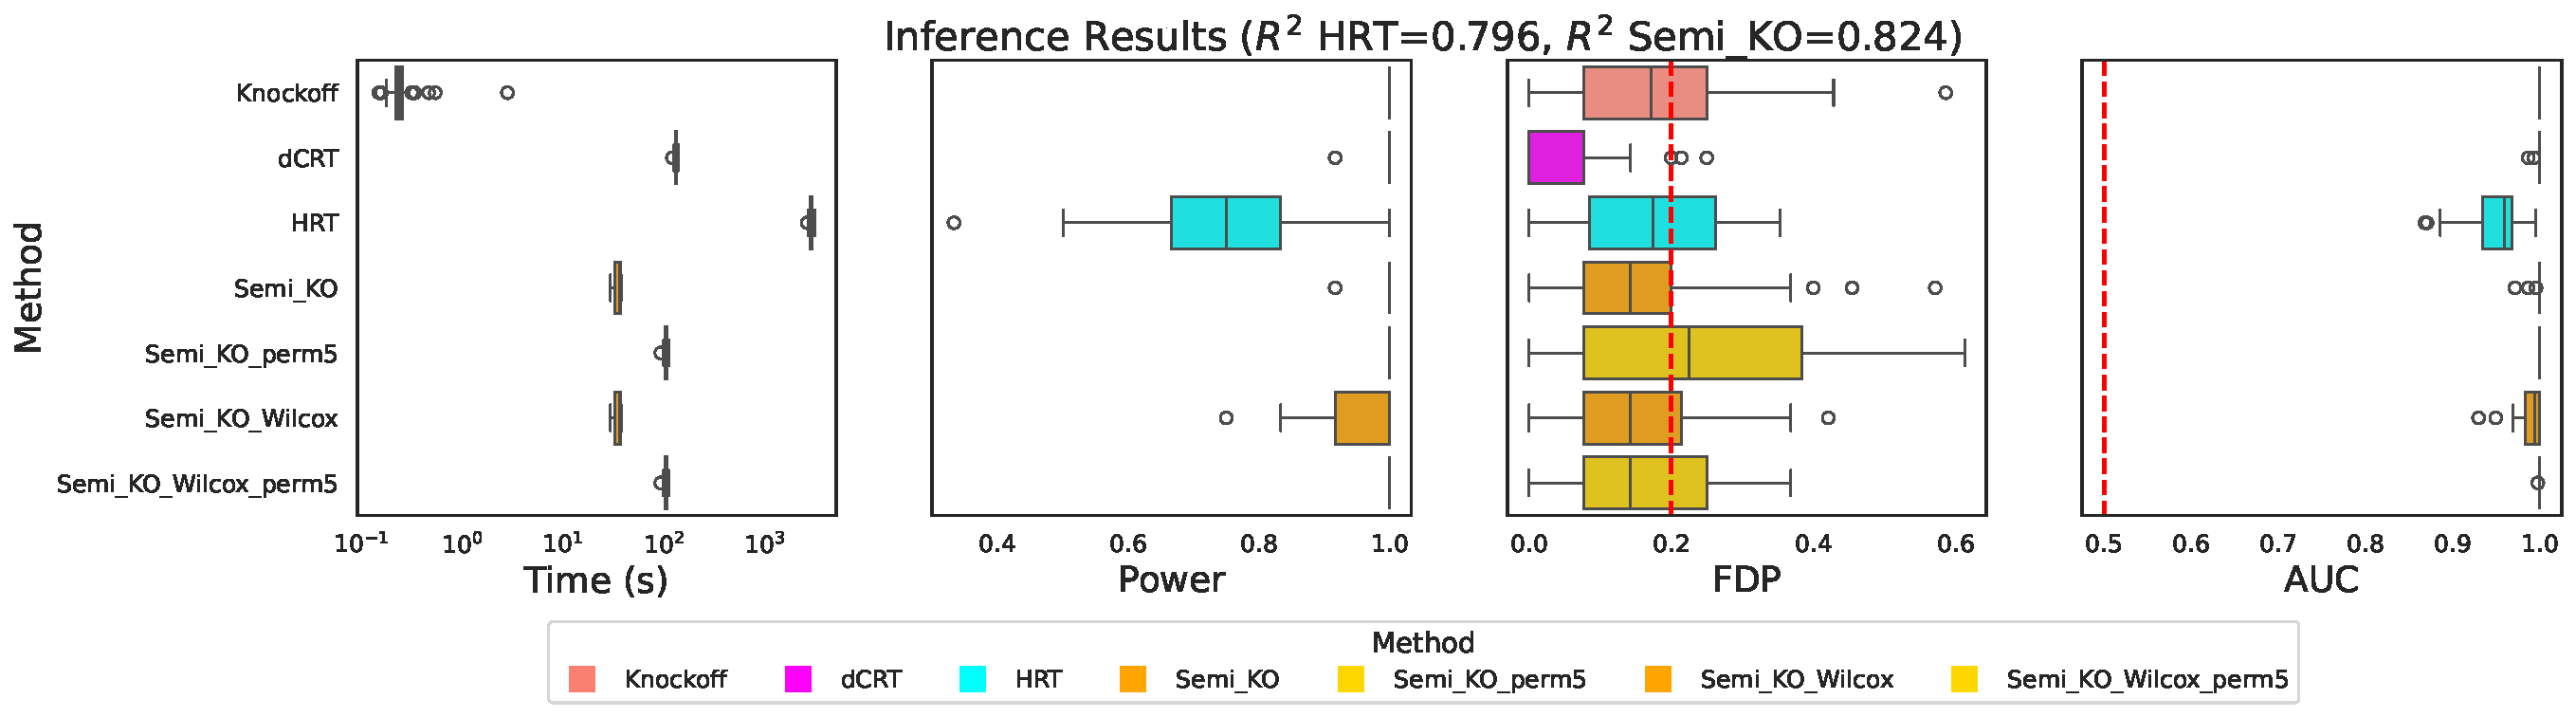
\includegraphics[width=1.03\textwidth]{images/exp_KO/adjacent_RF.pdf}
    \caption{\textbf{FDR adjacent support with Random Forest.} Let $X \sim \mathcal{N}(0,\Sigma)$ with $\Sigma^{ij} = 0.6^{|i-j|}$, and $y = \beta^\top X + \epsilon$, where the first $0.25p$ coordinates of $\beta$ are between $1$ and $2$ and the remaining entries are zero, and $\epsilon \sim \mathcal{N}(0,1)$. The black-box pretrained model $\widehat{m}$ is a random forest, achieving $R^2 = 0.796$ with a train-test split and $R^2 = 0.824$ without split.}
    \label{fig:app_KO_adj_rf}
\end{figure}



\subsubsection{Heavy-tails}

In this setting, the input features are no longer Gaussian. As a result, there is a reduced predictive performance compared to the adjacent setting. For instance, the $R^2$ of the neural network decreases from $R^2=0.965$ (with splitting: $R^2=0.964$) to $R^2=0.828$ (with splitting: $R^2=0.798$), and for gradient boosting from $R^2=0.910$ (with splitting: $R^2=0.884$) to $R^2=0.737$ (with splitting: $R^2=0.688$).

Nevertheless, we still observe that HRT loses power due to the train–test split. Overall, it is preferable to use \texttt{Semi-knockoffs} for FDR control rather than applying BH to the \texttt{Semi-Knockoffs-Wilcoxon} p-values, and the derandomization procedure further increases power.
%although the \texttt{Knockoffs} procedure remains powerful—since the relationship with $y$ is still linear and the Lasso Coefficient Difference is used as the test statistic—the variables are no longer exchangeable, and the symmetry under the null is not guaranteed. This explains the slight loss of FDR power \cite{blain2025knockoffsfaildiagnosingfixing}. Moreover, this non-Gaussianity also   
Note that in this linear setting, the knockoffs are powerful since they rely on the Lasso coefficient difference. However, Gaussian knockoff variables are no longer valid here, so the FDR is not theoretically controlled.


\begin{figure}
    \centering
    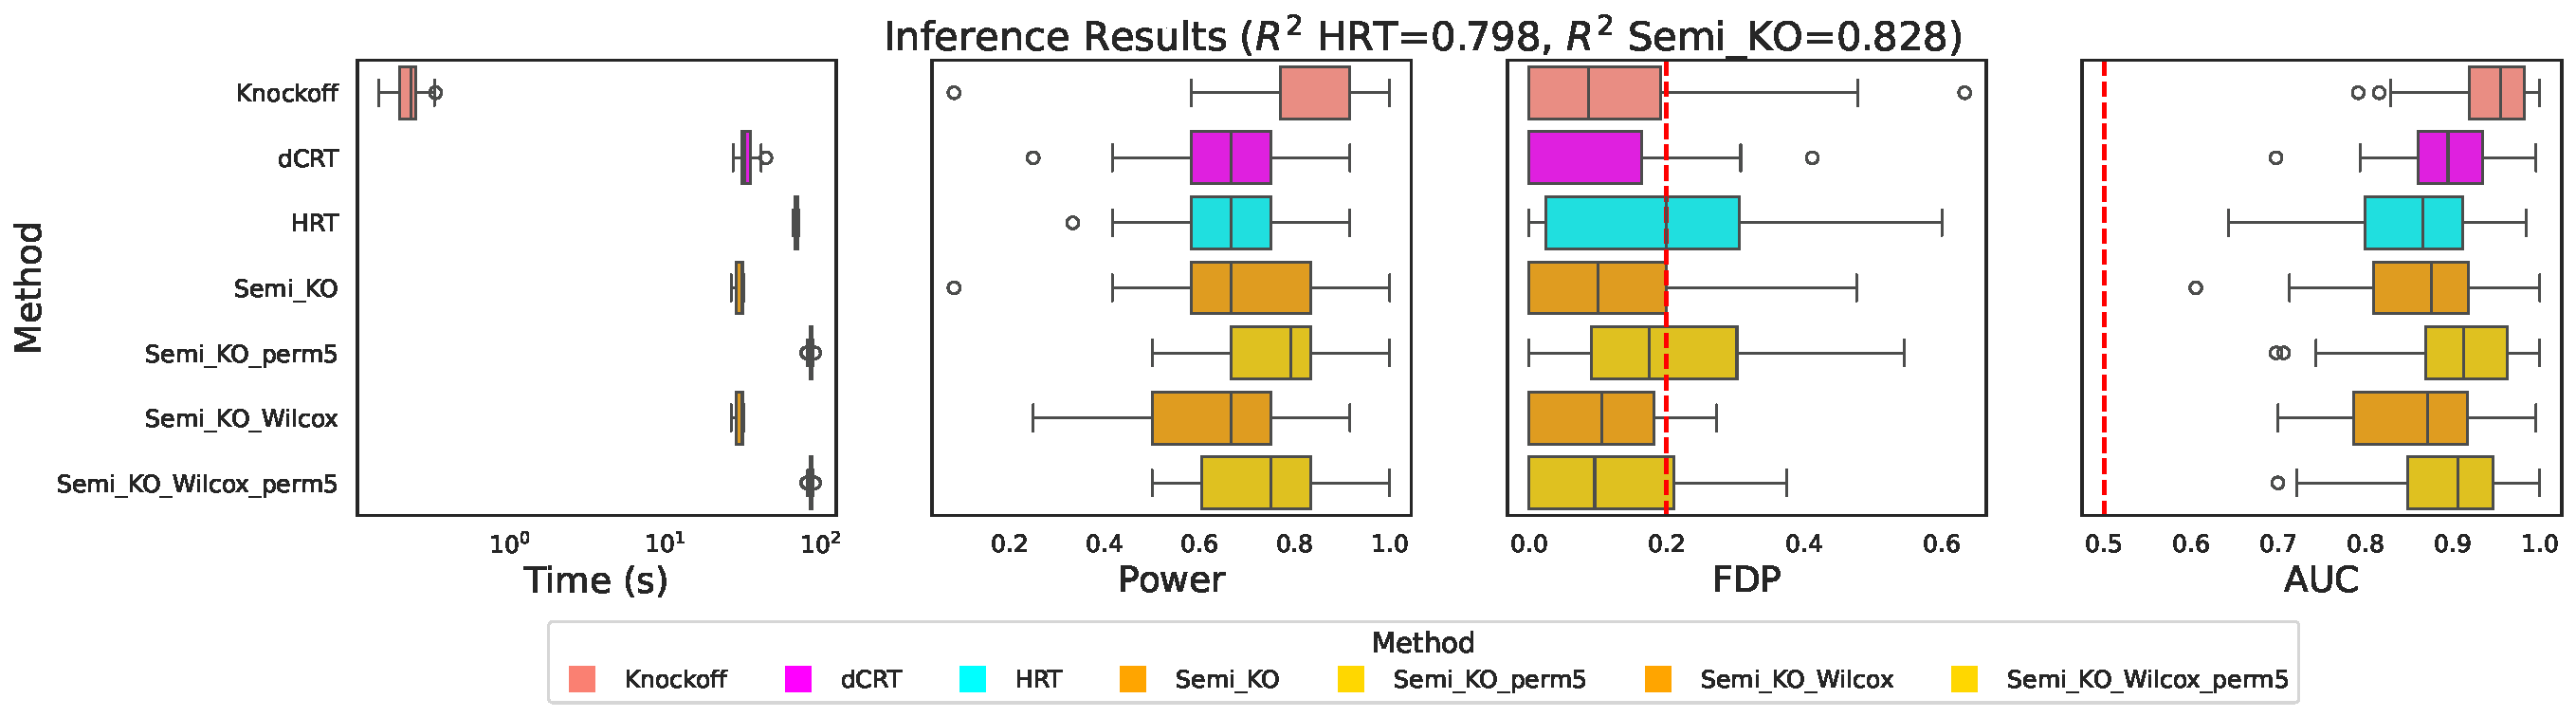
\includegraphics[width=1.03\textwidth]{images/exp_KO/nongauss_NN.pdf}
    \caption{\textbf{FDR heavy-tailed with Neural Networks.} Let $X = \Sigma^{1/2} Z$, where $Z$ has i.i.d.\ t-Student entries $Z_{ij} \sim t_3$ and $\Sigma_{ij} = 0.6^{|i-j|}$.  We generate $y = \beta^\top X + \epsilon$, where the first $0.25p$ coordinates of $\beta$ lie in $[1,2]$ and the remaining entries are zero, with $\epsilon \sim \mathcal{N}(0,1)$. The black-box pretrained model $\widehat{m}$ is a neural network, achieving $R^2 = 0.798$ with a train-test split and $R^2 = 0.828$ without split.
}
    \label{fig:app_KO_nongaus_NN}
\end{figure}



\begin{figure}
    \centering
    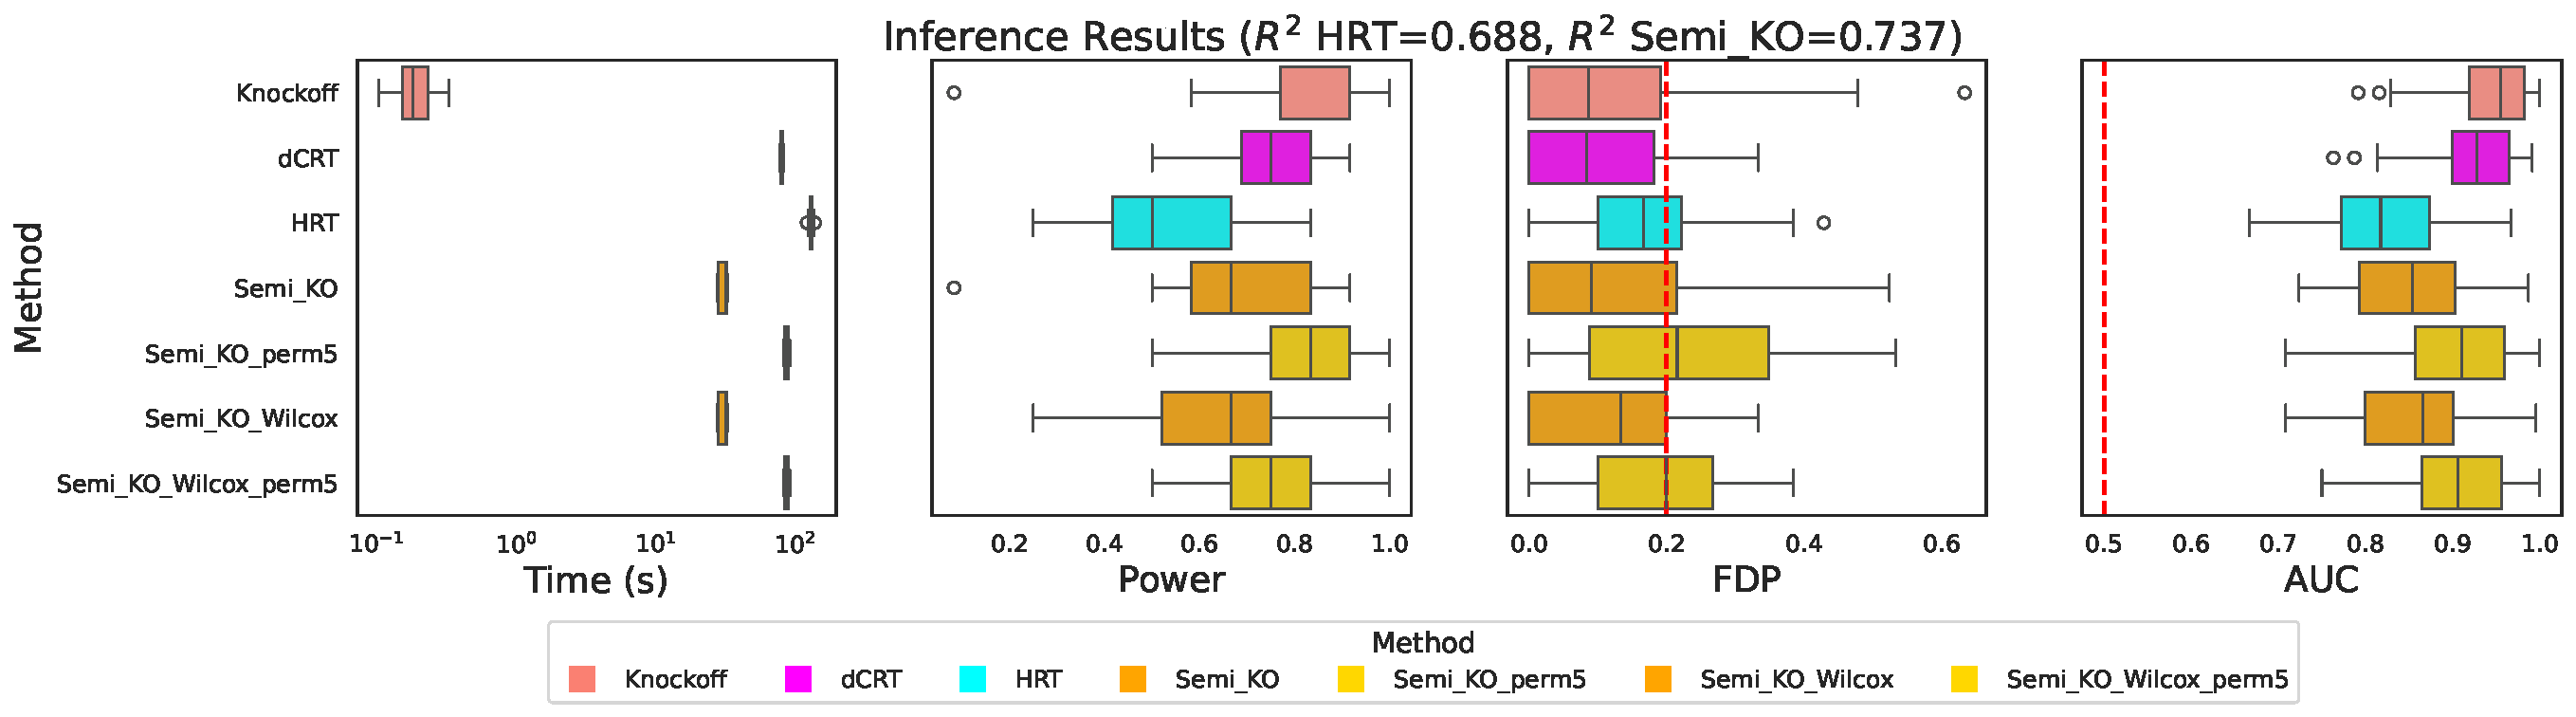
\includegraphics[width=1.03\textwidth]{images/exp_KO/nongauss_GB.pdf}
    \caption{\textbf{FDR heavy-tailed with Gradient Boosting.} Let $X = \Sigma^{1/2} Z$, where $Z$ has i.i.d.\ t-Student entries $Z_{ij} \sim t_3$ and $\Sigma_{ij} = 0.6^{|i-j|}$.  We generate $y = \beta^\top X + \epsilon$, where the first $0.25p$ coordinates of $\beta$ lie in $[1,2]$ and the remaining entries are zero, with $\epsilon \sim \mathcal{N}(0,1)$. The black-box pretrained model $\widehat{m}$ is a gradient boosting, achieving $R^2 = 0.688$ with a train-test split and $R^2 = 0.737$ without split.
}
    \label{fig:app_KO_nongaus_GB}
\end{figure}


\begin{figure}
    \centering
    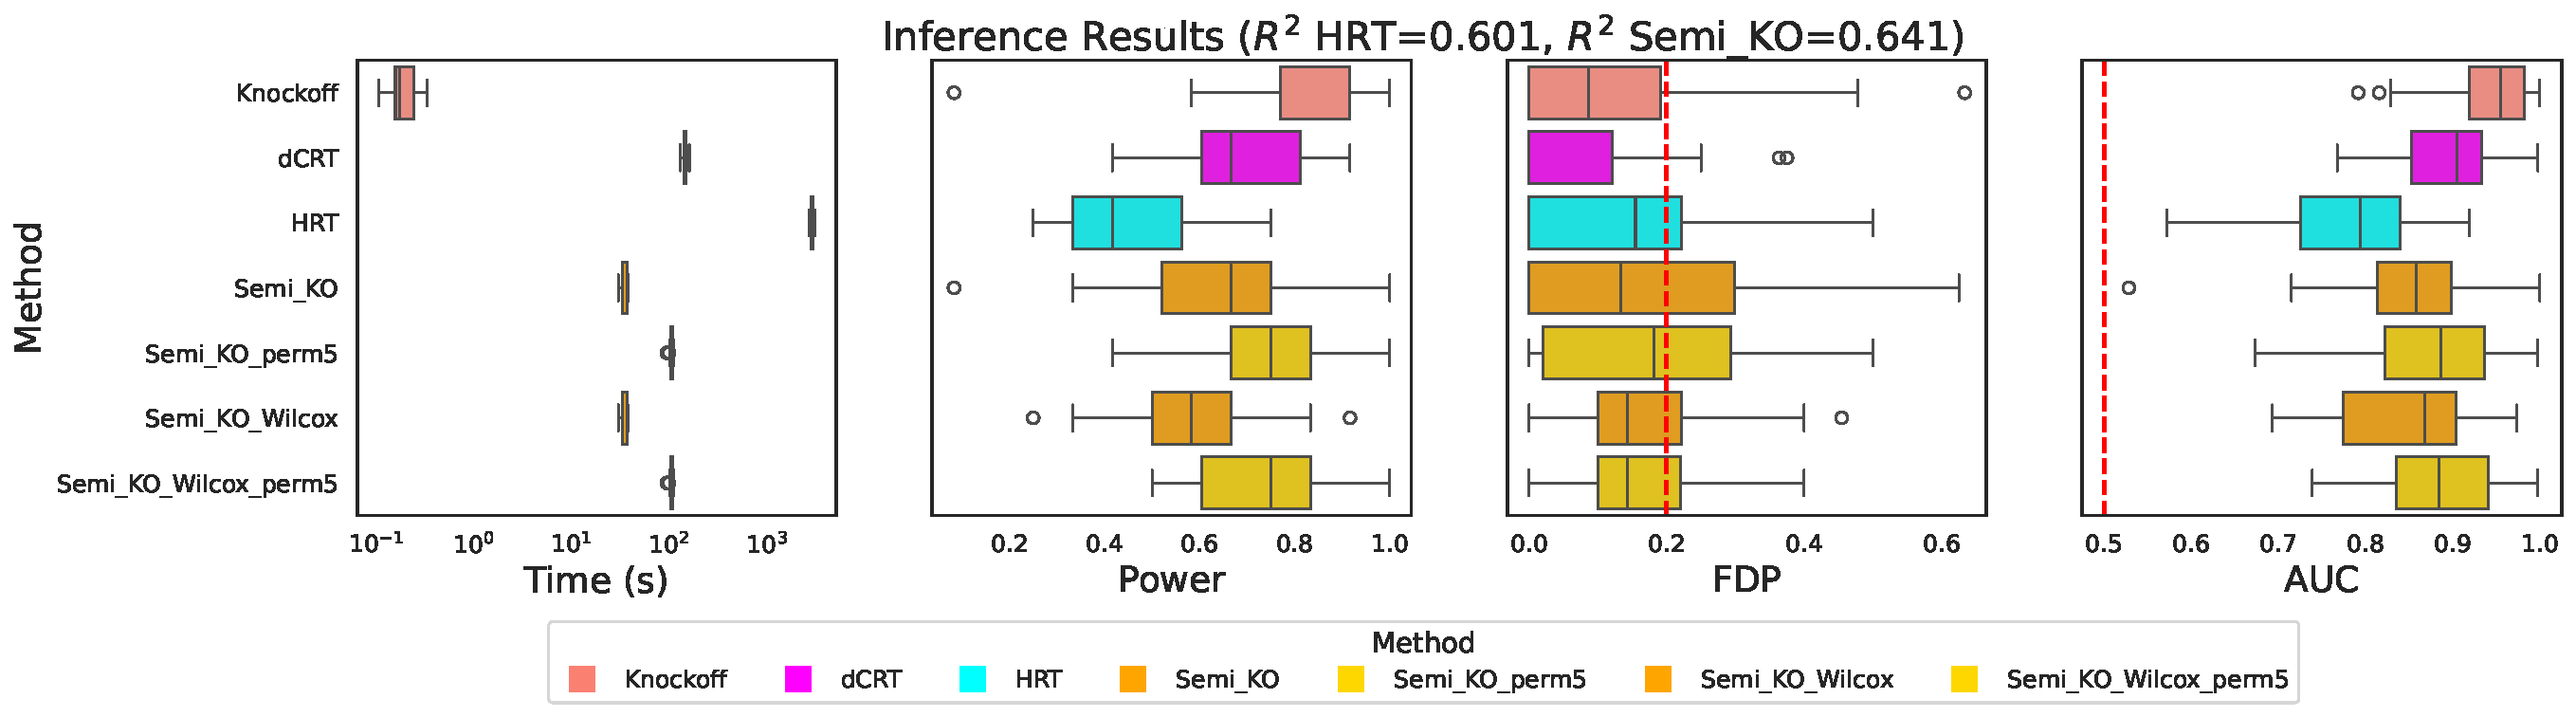
\includegraphics[width=1.03\textwidth]{images/exp_KO/nongauss_RF.pdf}
    \caption{\textbf{FDR heavy-tailed with Random Forest.} Let $X = \Sigma^{1/2} Z$, where $Z$ has i.i.d.\ t-Student entries $Z_{ij} \sim t_3$ and $\Sigma_{ij} = 0.6^{|i-j|}$.  We generate $y = \beta^\top X + \epsilon$, where the first $0.25p$ coordinates of $\beta$ lie in $[1,2]$ and the remaining entries are zero, with $\epsilon \sim \mathcal{N}(0,1)$. The black-box pretrained model $\widehat{m}$ is a random forest, achieving $R^2 = 0.601$ with a train-test split and $R^2 = 0.641$ without split.
}
    \label{fig:app_KO_nongaus_RF}
\end{figure}




%\subsection{Identification capacity}


%\ar{Change the captions!!!}


%\begin{figure}
%    \centering
%    \includegraphics[width=0.95\textwidth]{images/experiments_p_val/AUC_hidim_p100_cor0.6.pdf}
%    \caption{\textbf{Double Robustness and identification capacity of Semi-knockoffs:} The data-generating model is $y = X^\top \beta + \epsilon$, with $\epsilon \sim \mathcal{N}(0, 0.5)$ and $\beta$ $0.5$-sparse randomly sampled with half of the values equally sampled from $0.3$ to $1$, and the other half from $-0.8$ to $-0.2$. We use $n = 500$ samples with $X \sim \mathcal{N}(0, \Sigma)$, where $\Sigma^{i,j} = 0.5^{|i-j|}$ and $X\in \mathbb{R}^{50}$.
% }
%    \label{fig:AUC_hidims}
%\end{figure}



%\begin{figure}
%    \centering
%    \includegraphics[width=0.95\textwidth]{images/experiments_p_val/AUC_poly_p50_cor0.6.pdf}
%    \caption{...
% }
%    \label{fig:AUC_poly}
%\end{figure}




\subsection{Real data experiments}\label{app:wdbc}


The \emph{Wisconsin Diagnostic Breast Cancer} (WDBC) dataset consists of $n=569$ patient samples with $p=30$ numeric features of individual cells, obtained from a minimally invasive fine needle aspirate, to discriminate benign from malignant breast lumps. This dataset is widely used for binary classification tasks in medical informatics \citep{wdbc1995}.

Since the underlying distribution is unknown, we estimate the type-I error by adding an artificial null feature correlated at $0.6$ with the original inputs. We present results for computation time, number of discoveries, and type-I error using Random Forests, Neural Networks, and Gradient Boosting (Figures~\ref{fig:real_app_RF}, \ref{fig:real_app_NN}, and \ref{fig:real_app_GB}, respectively). The conclusions are consistent with those from the simulated settings. The additive term correction is overly restrictive in practice and yields no discoveries (\texttt{\_sqrt}). \texttt{LOCO-W} does not control the error. The \texttt{dCRT} makes no discoveries with Neural Networks or Gradient Boosting in the distillation step. Computationally, Semi-knockoffs should provide an advantage since no refitting of the complex model is required; however, in these simulations we used default implementations, so the benefit is less noticeable.


\begin{figure}
    \centering
    %\hspace{-1.5em}
    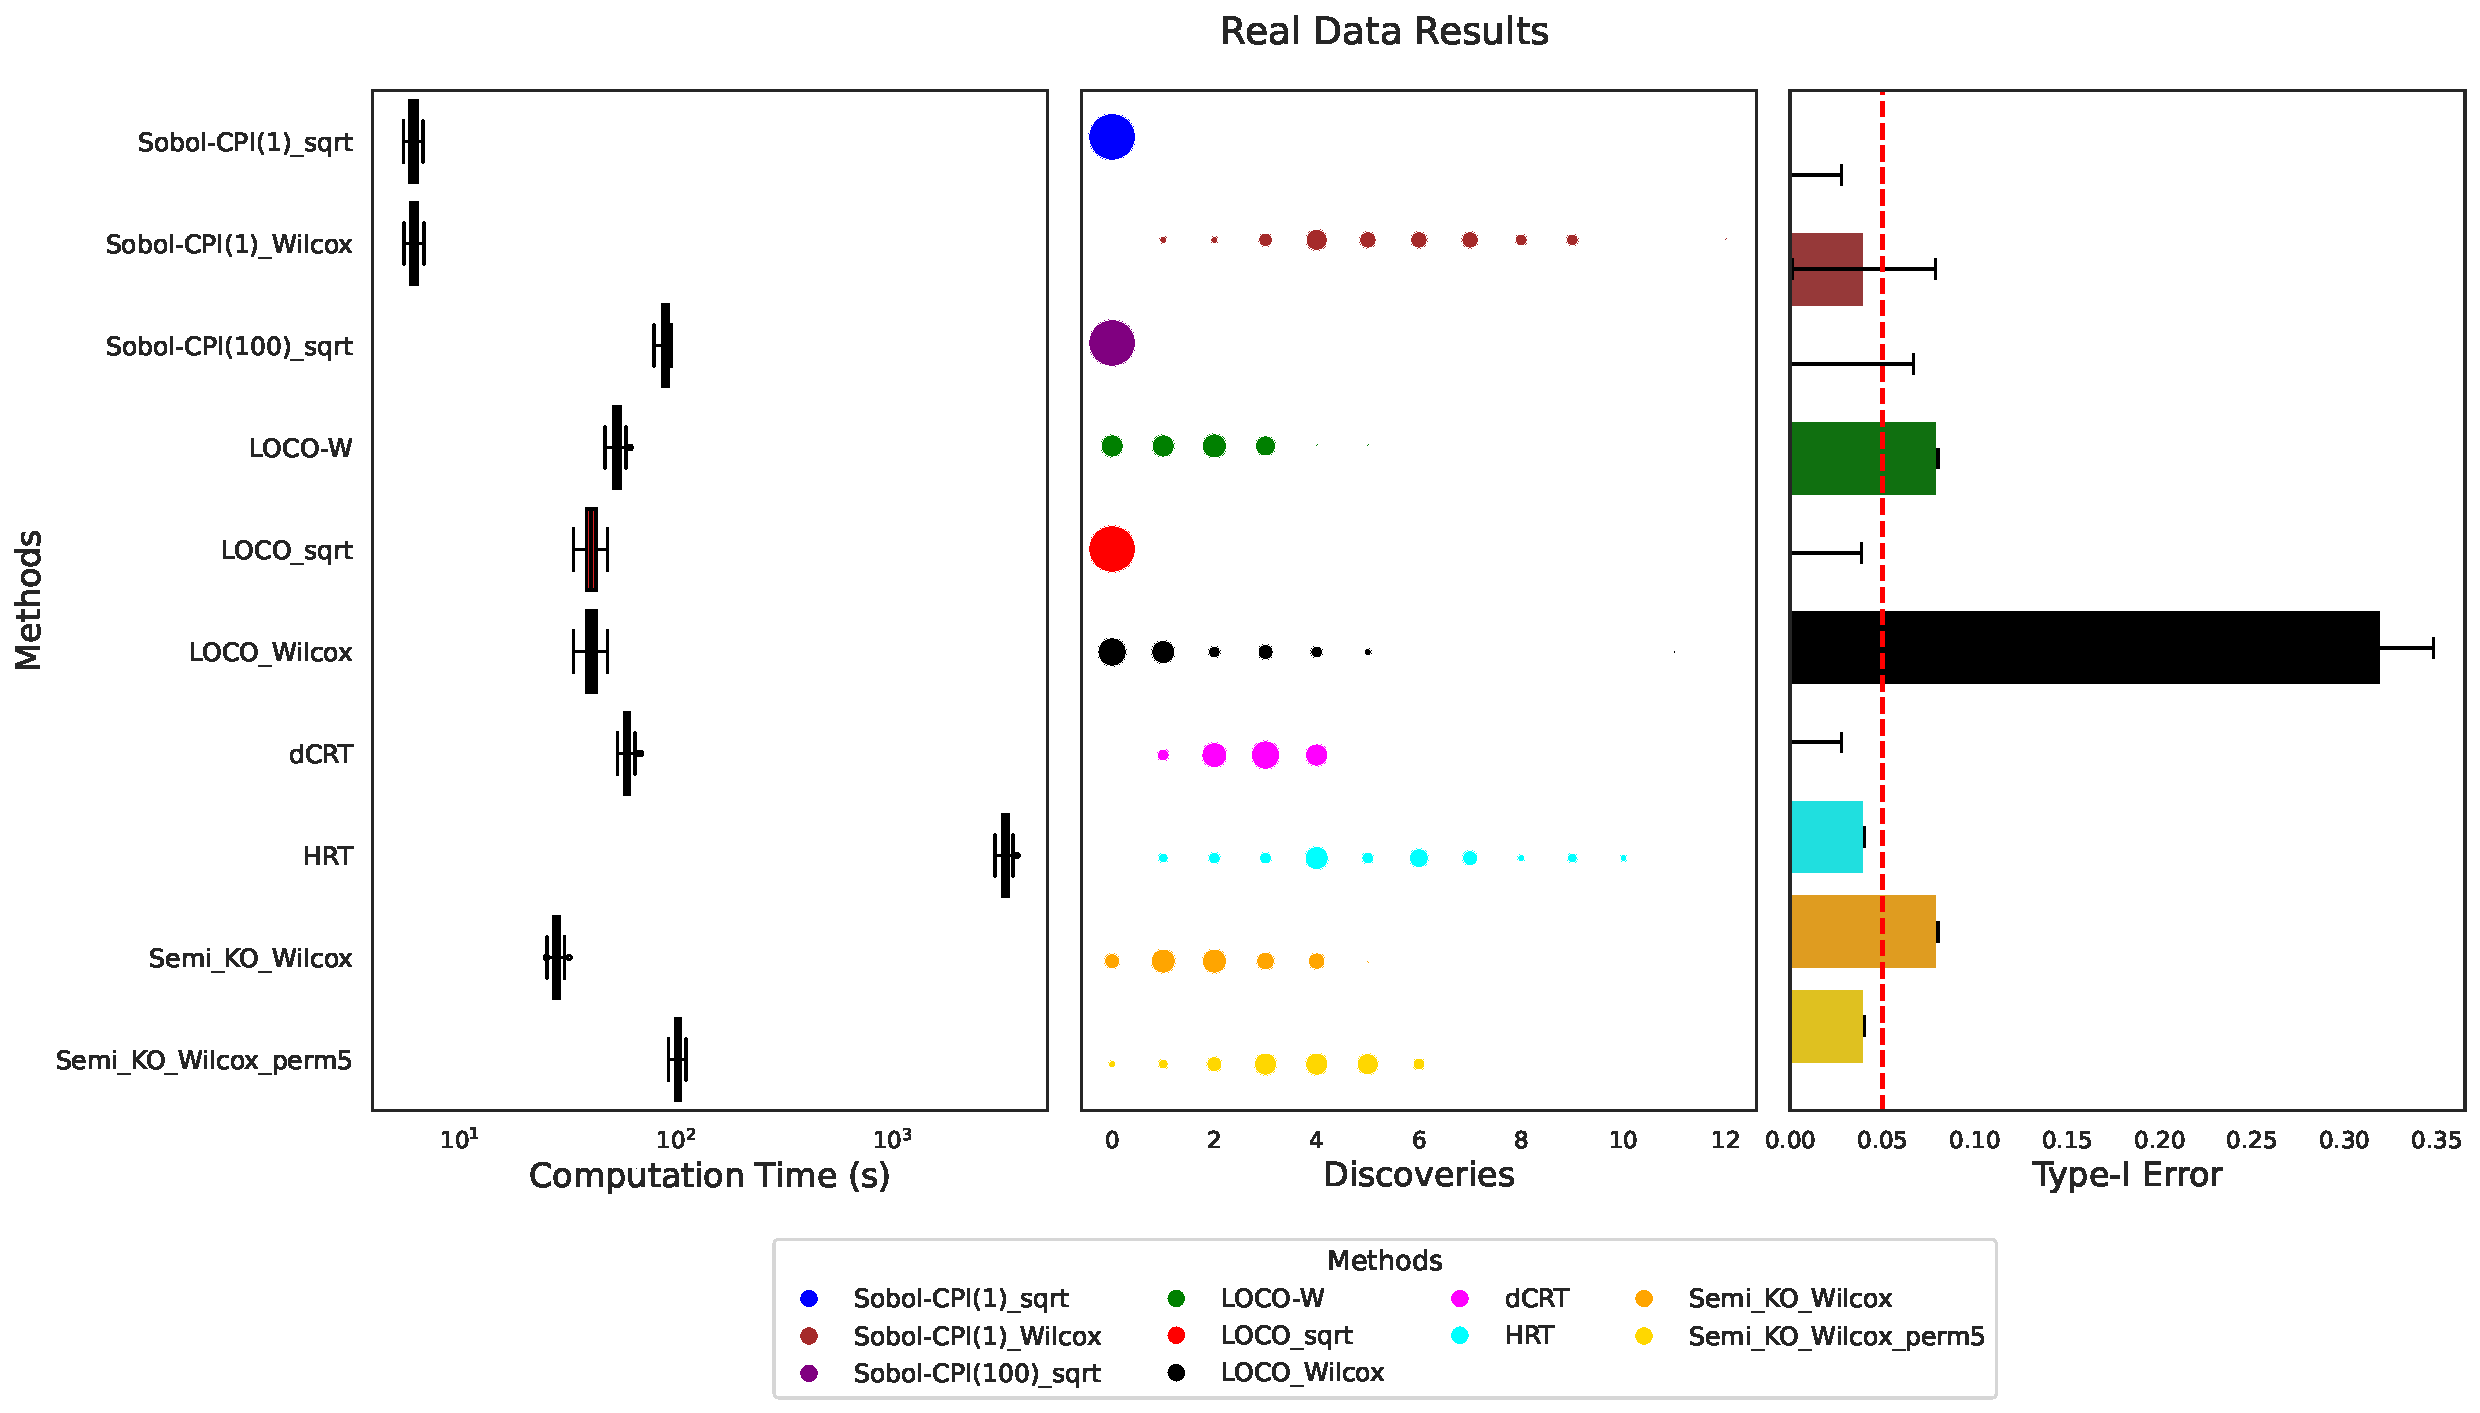
\includegraphics[width=0.8\textwidth]{images/real_data/scatter_wdbc_RF.pdf}
    \caption{\textbf{Discoveries on real data using a Random Forest.} Left: computation time; middle: number of discoveries; right: type-I error, estimated using an artificial null feature correlated at $0.6$ with the original features. Semi-knockoffs makes discoveries while controlling the error.
}
    \label{fig:real_app_RF}
\end{figure}


\begin{figure}
    \centering
    %\hspace{-1.5em}
    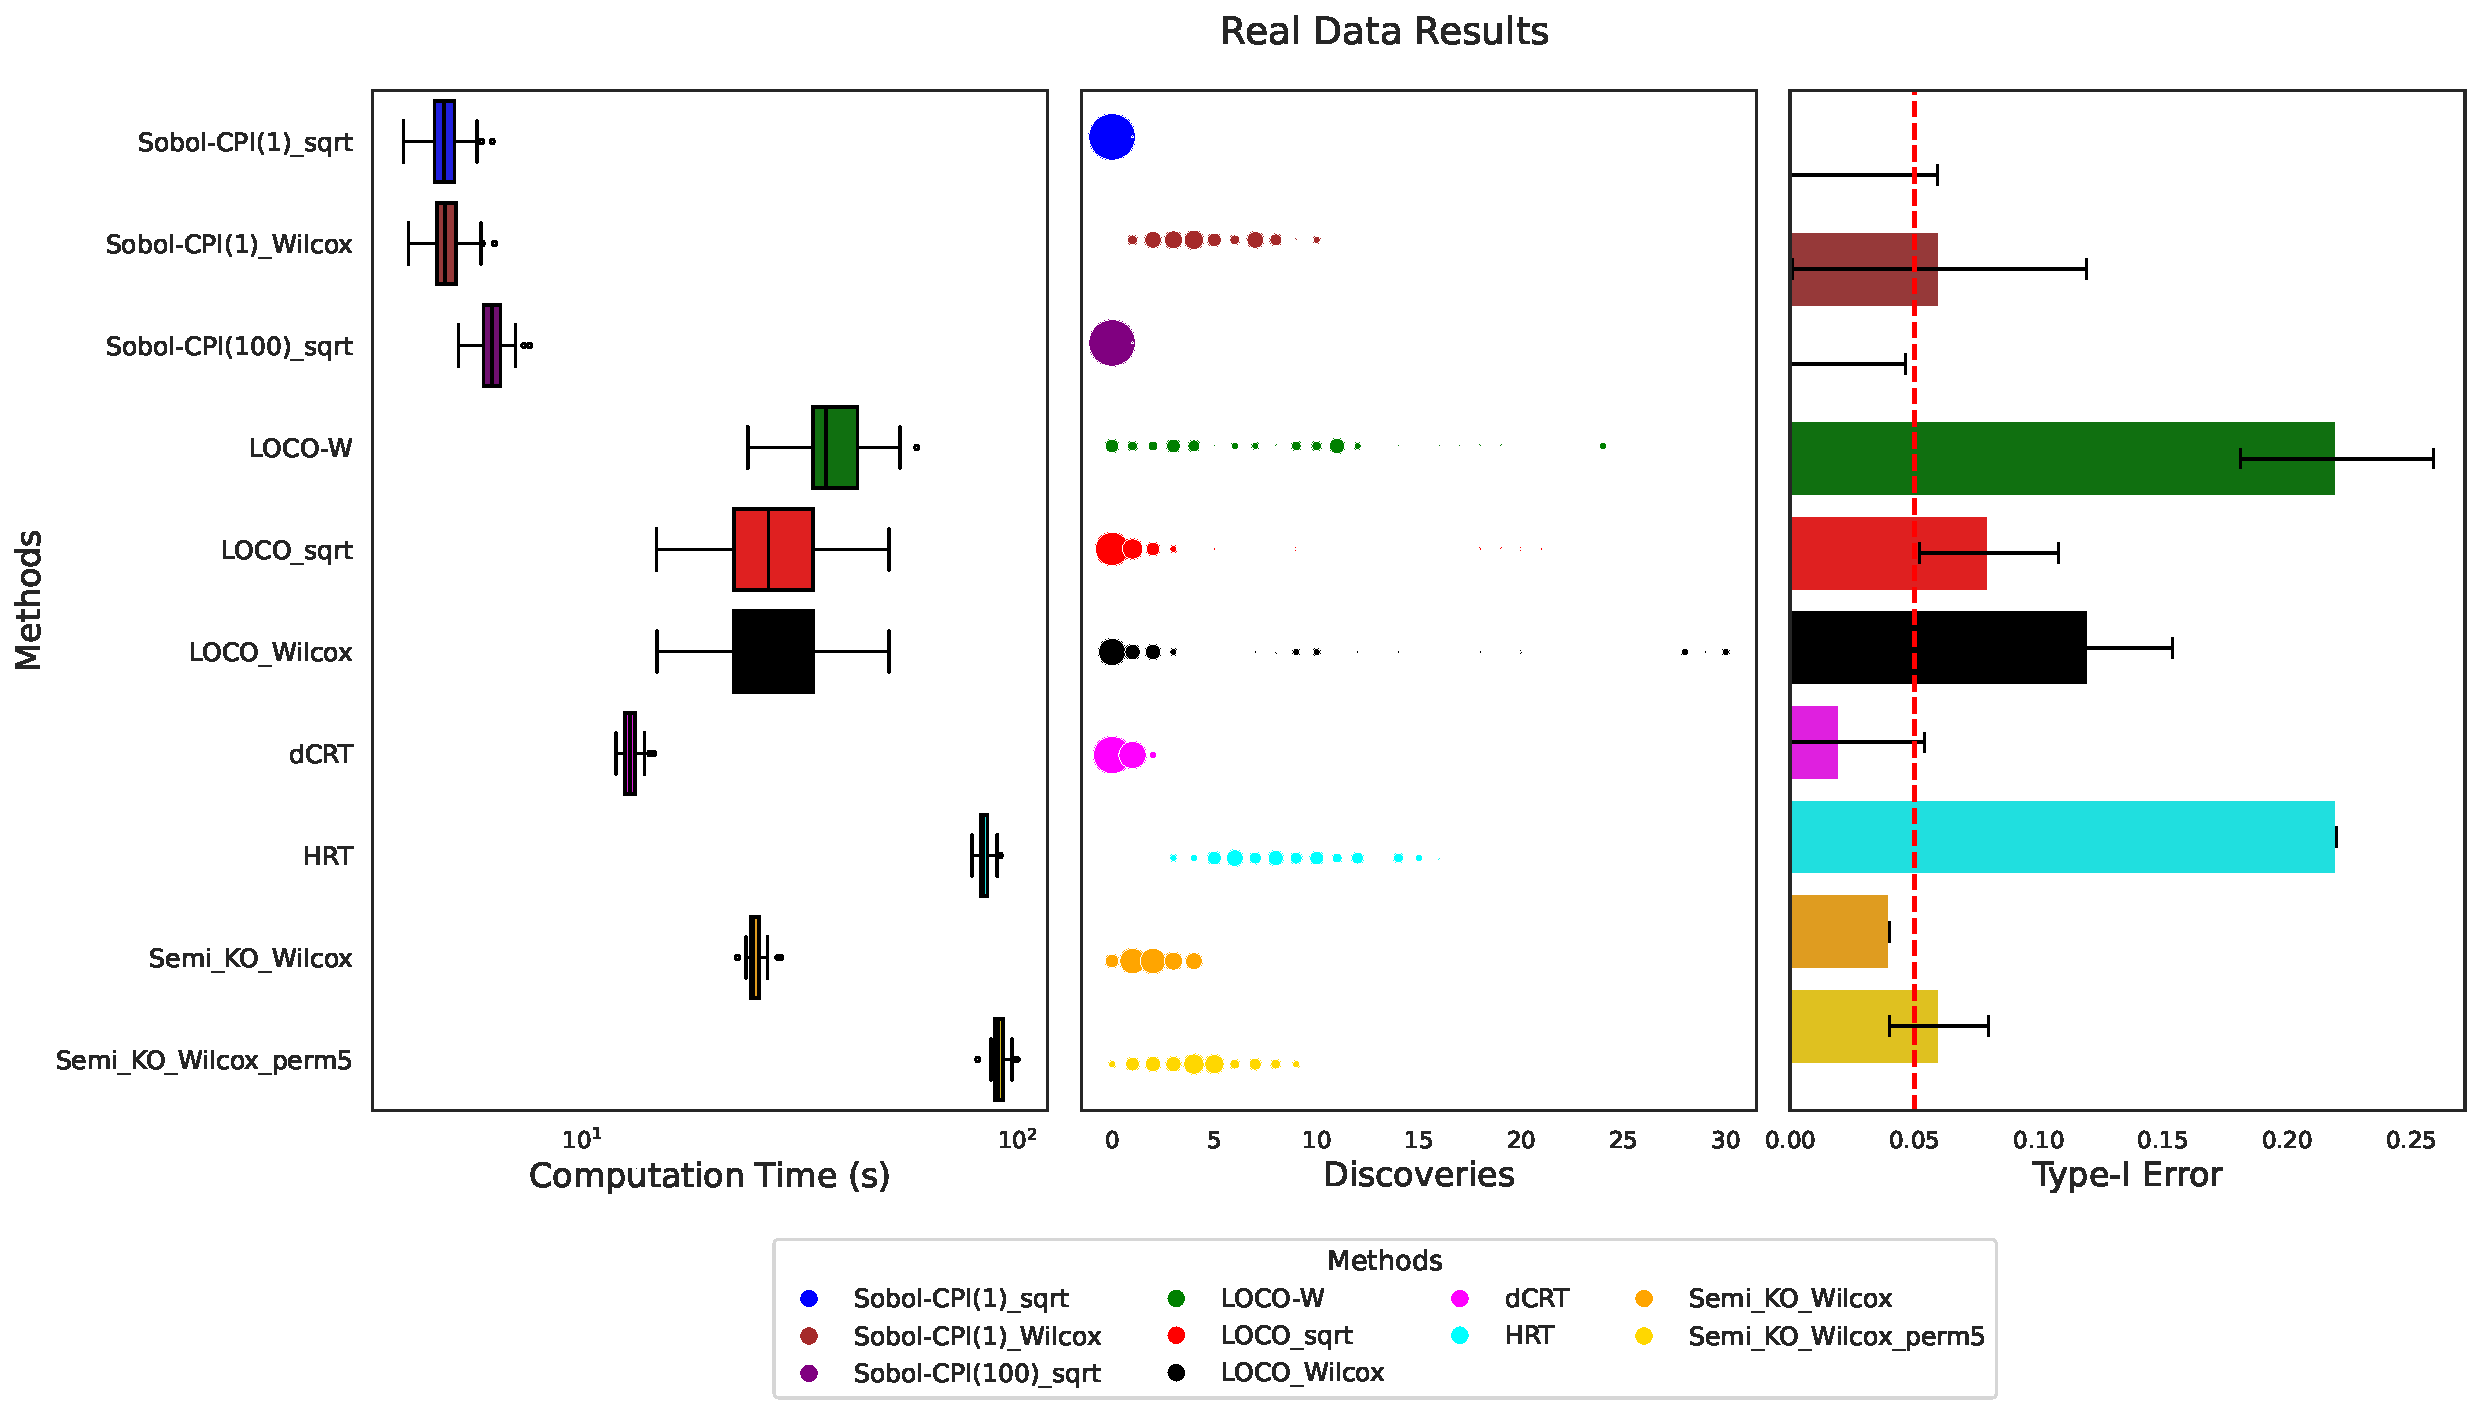
\includegraphics[width=0.8\textwidth]{images/real_data/scatter_wdbc_NN.pdf}
    \caption{\textbf{Discoveries on real data using a Neural Network.} Left: computation time; middle: number of discoveries; right: type-I error, estimated using an artificial null feature correlated at $0.6$ with the original features. Semi-knockoffs makes discoveries while controlling the error.
}
    \label{fig:real_app_NN}
\end{figure}

\begin{figure}
    \centering
    %\hspace{-1.5em}
    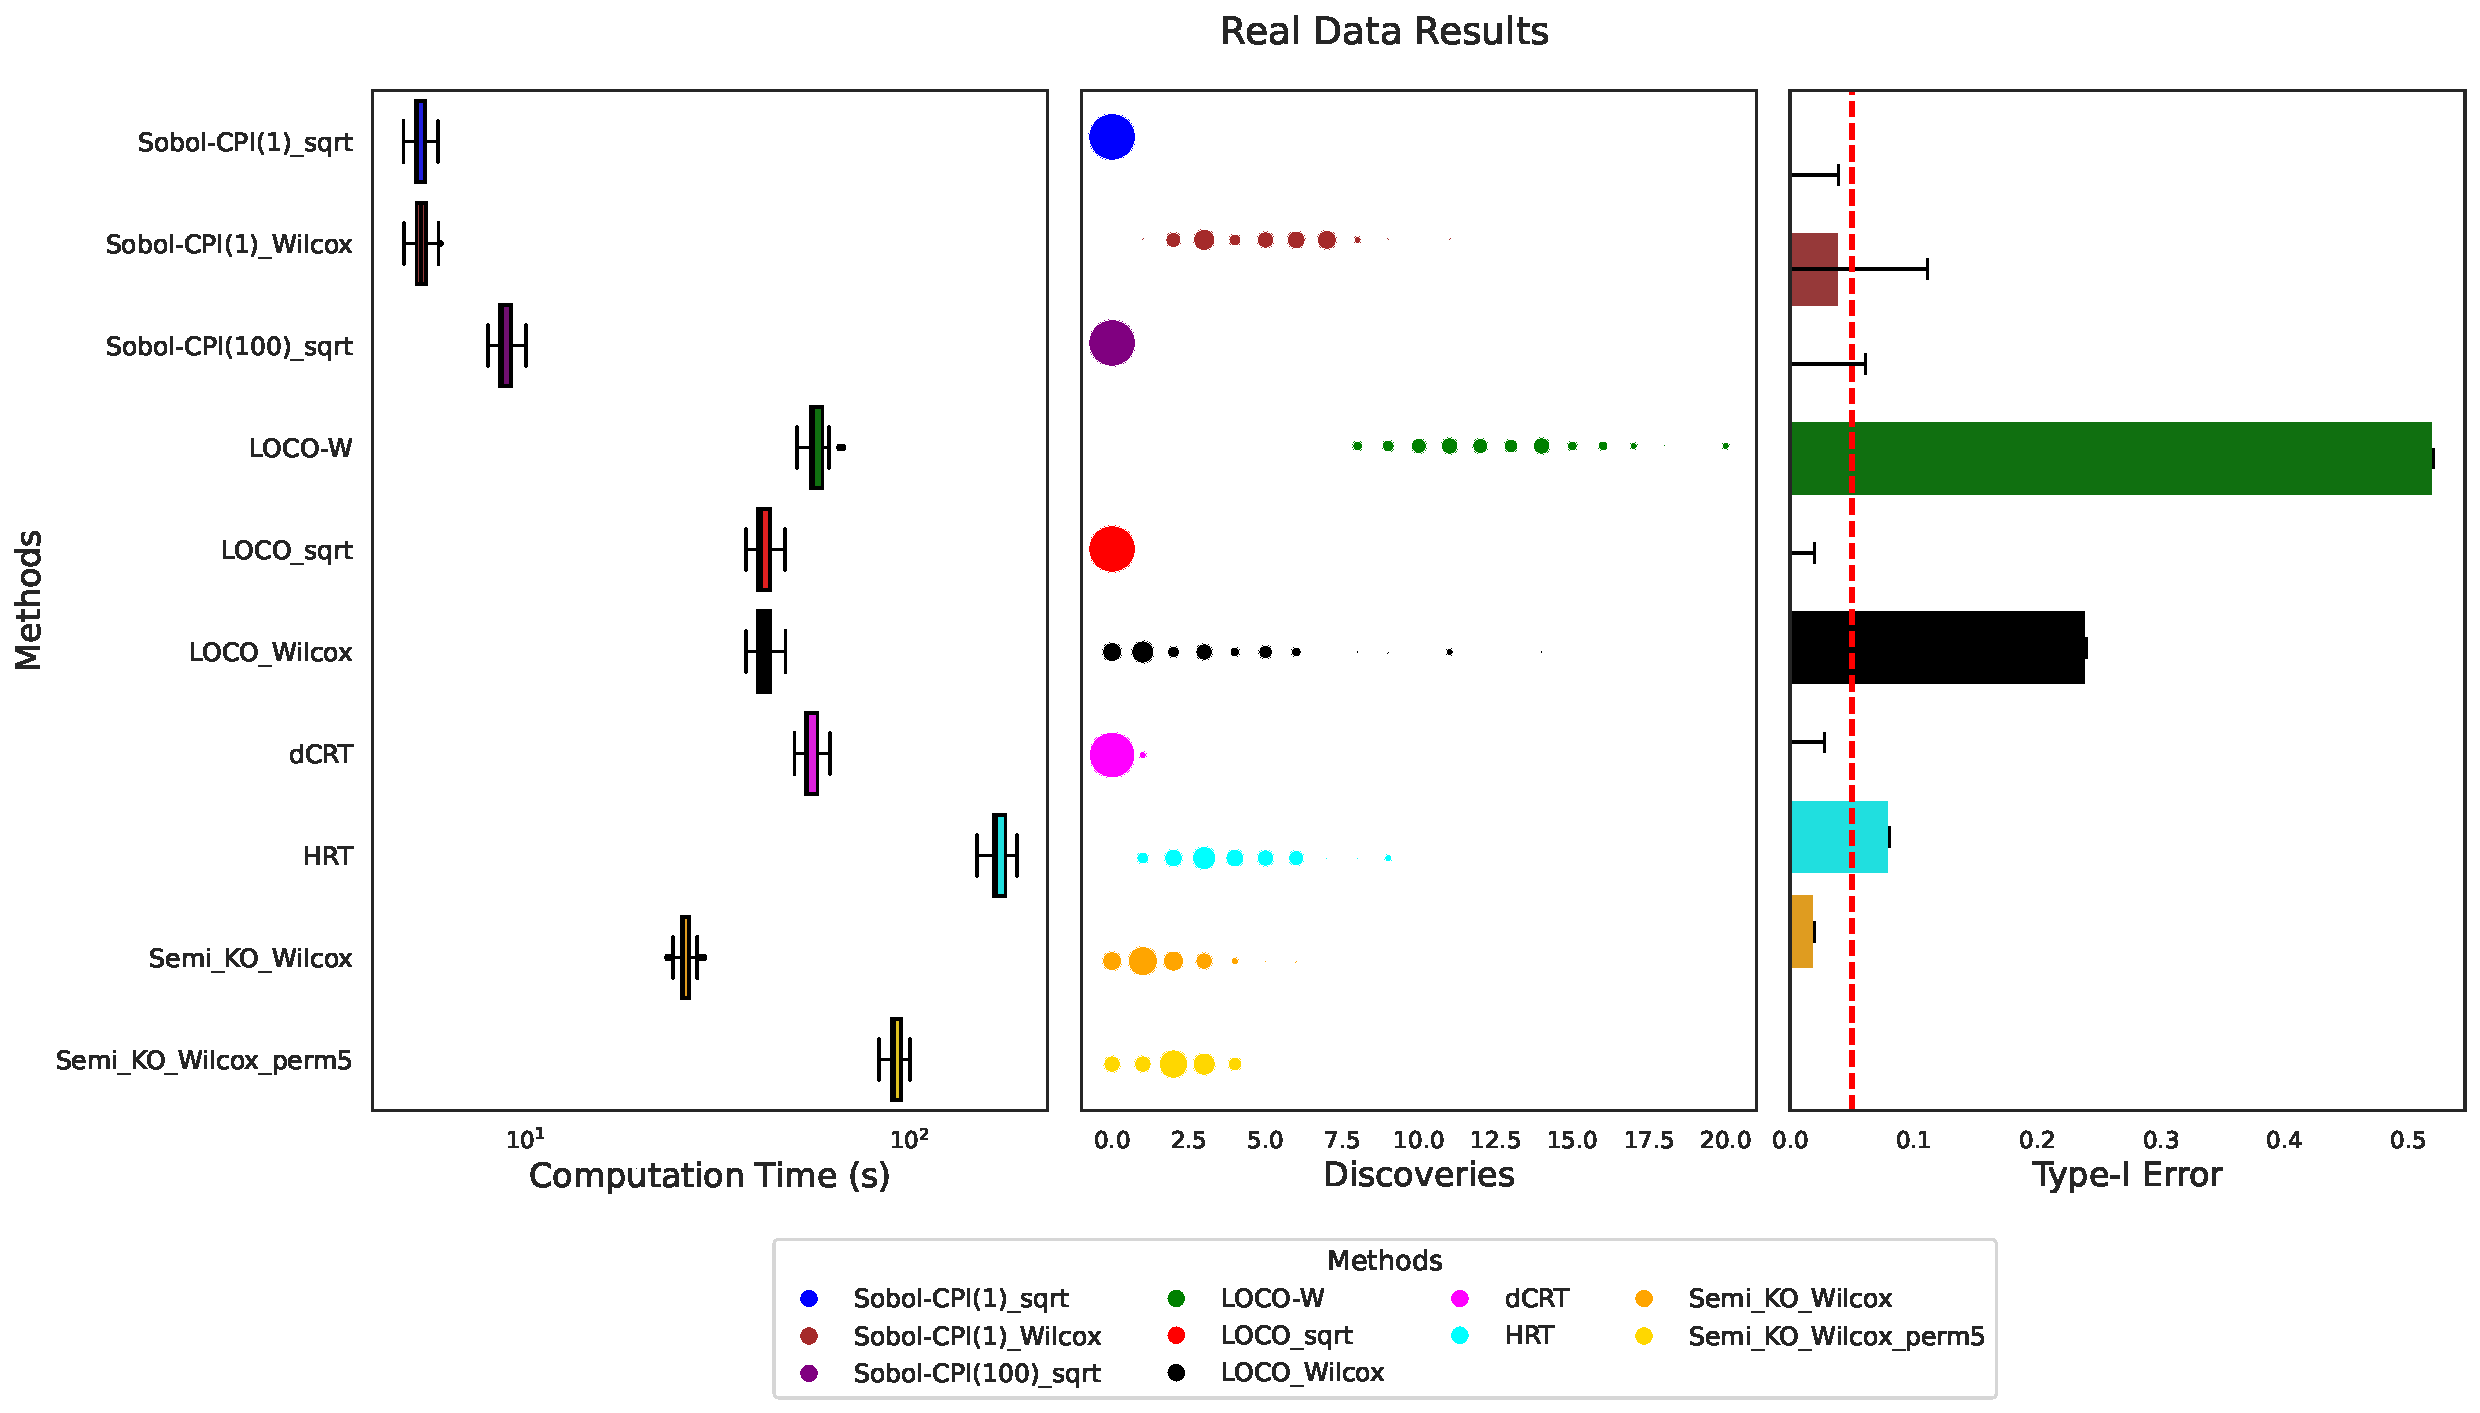
\includegraphics[width=0.8\textwidth]{images/real_data/scatter_wdbc_GB.pdf}
    \caption{\textbf{Discoveries on real data using a Gradient Boosting.} Left: computation time; middle: number of discoveries; right: type-I error, estimated using an artificial null feature correlated at $0.6$ with the original features. Semi-knockoffs makes discoveries while controlling the error.
}
    \label{fig:real_app_GB}
\end{figure}


\end{document}

% This document was modified from the file originally made available by
% Pat Langley and Andrea Danyluk for ICML-2K. This version was created
% by Iain Murray in 2018, and modified by Alexandre Bouchard in
% 2019 and 2021 and by Csaba Szepesvari, Gang Niu and Sivan Sabato in 2022.
% Modified again in 2023 and 2024 by Sivan Sabato and Jonathan Scarlett.
% Previous contributors include Dan Roy, Lise Getoor and Tobias
% Scheffer, which was slightly modified from the 2010 version by
% Thorsten Joachims & Johannes Fuernkranz, slightly modified from the
% 2009 version by Kiri Wagstaff and Sam Roweis's 2008 version, which is
% slightly modified from Prasad Tadepalli's 2007 version which is a
% lightly changed version of the previous year's version by Andrew
% Moore, which was in turn edited from those of Kristian Kersting and
% Codrina Lauth. Alex Smola contributed to the algorithmic style files.
